
%% $Id$

\documentclass[12pt,a4paper,fleqn]{report}
\usepackage{latexsym,graphicx,../iman,../extra,../ttbox,../proof,../rail,../railsetup,../isar,../pdfsetup}

\title{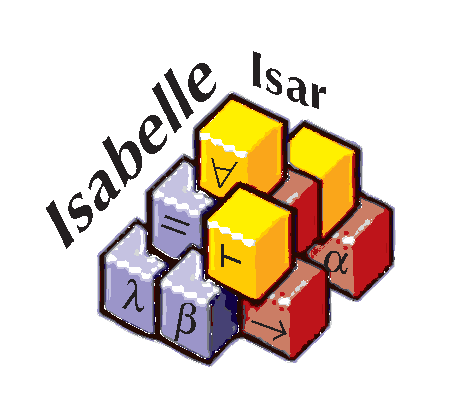
\includegraphics[scale=0.5]{isabelle_isar} \\[4ex] The Isabelle/Isar Reference Manual}
\author{\emph{Markus Wenzel} \\ TU M\"unchen}

\makeindex

\newcommand{\isastyle}{\small\tt\slshape}
\newcommand{\isa}[1]{\emph{\isastyle #1}}
\newcommand{\isamath}[1]{\emph{$#1$}}
\newcommand{\isasymColon}{\isamath{\mathrel{::}}}
\newcommand{\isasymRightarrow}{\isamath{\Rightarrow}}
\newcommand{\isasymleftharpoondown}{\isamath{\leftharpoondown}}
\newcommand{\isasymrightharpoonup}{\isamath{\rightharpoonup}}
\newcommand{\isasymrightleftharpoons}{\isamath{\rightleftharpoons}}
\newcommand{\isasymequiv}{\isamath{\equiv}}
\newcommand{\isasymsubseteq}{\isamath{\subseteq}}

\railterm{percent,ppercent,underscore,lbrace,rbrace,atsign}
\railterm{ident,longident,symident,var,textvar,typefree,typevar,nat,string,verbatim,keyword}
\railterm{name,nameref,text,type,term,prop,atom}

\railalias{ident}{\railtoken{ident}}
\railalias{longident}{\railtoken{longident}}
\railalias{symident}{\railtoken{symident}}
\railalias{var}{\railtoken{var}}
\railalias{textvar}{\railtoken{textvar}}
\railalias{typefree}{\railtoken{typefree}}
\railalias{typevar}{\railtoken{typevar}}
\railalias{nat}{\railtoken{nat}}
\railalias{string}{\railtoken{string}}
\railalias{verbatim}{\railtoken{verbatim}}
\railalias{keyword}{\railtoken{keyword}}

\railalias{name}{\railqtoken{name}}
\railalias{nameref}{\railqtoken{nameref}}
\railalias{text}{\railqtoken{text}}
\railalias{type}{\railqtoken{type}}
\railalias{term}{\railqtoken{term}}
\railalias{prop}{\railqtoken{prop}}
\railalias{atom}{\railqtoken{atom}}

\newcommand{\drv}{\mathrel{\vdash}}
\newcommand{\edrv}{\mathop{\drv}\nolimits}
\newcommand{\Or}{\mathrel{\;|\;}}

\renewcommand{\vec}[1]{\overline{#1}}

\setcounter{secnumdepth}{2} \setcounter{tocdepth}{2}

\pagestyle{headings}
\sloppy
\binperiod     %%%treat . like a binary operator

\renewcommand{\phi}{\varphi}

%\includeonly{}


\begin{document}

\underscoreoff

\maketitle 

\pagenumbering{roman} \tableofcontents \clearfirst


\chapter{Introduction}

\section{Quick start}

Isar is already part of Isabelle (as of version Isabelle99, or later).  The
\texttt{isabelle} binary provides option \texttt{-I} to run the Isar
interaction loop at startup, rather than the plain ML top-level.  Thus the
quickest way to do anything with Isabelle/Isar is as follows:
\begin{ttbox}
isabelle -I HOL\medskip
\out{> Welcome to Isabelle/HOL (Isabelle99)}\medskip
theory Foo = Main:
constdefs foo :: nat  "foo == 1";
lemma "0 < foo" by (simp add: foo_def);
end
\end{ttbox}
Note that any Isabelle/Isar command may be retracted by \texttt{undo}.

Plain TTY-based interaction like this used to be quite feasible with
traditional tactic based theorem proving, but developing Isar documents
demands some better user-interface support.  \emph{Proof~General}\index{Proof
  General} of LFCS Edinburgh \cite{proofgeneral} offers a generic Emacs-based
environment for interactive theorem provers that does all the cut-and-paste
and forward-backward walk through the document in a very neat way.  Note that
in Isabelle/Isar, the current position within a partial proof document is more
informative than the actual proof state.  Thus Proof~General provides the
canonical working environment for Isabelle/Isar, both for getting acquainted
(e.g.\ by replaying existing Isar documents) and serious production work.

\medskip

The easiest way to use Proof~General is to make it the default Isabelle user
interface.  Just say something like this in your Isabelle settings file (cf.\ 
\cite{isabelle-sys}):
\begin{ttbox}
ISABELLE_INTERFACE=\$ISABELLE_HOME/contrib/ProofGeneral/isar/interface
PROOFGENERAL_OPTIONS=""
\end{ttbox}
You may have to change \texttt{\$ISABELLE_HOME/contrib/ProofGeneral} to the
actual installation directory of Proof~General.  From now on, the capital
\texttt{Isabelle} executable refers to the \texttt{ProofGeneral/isar}
interface.  Its usage is as follows:
\begin{ttbox}
Usage: interface [OPTIONS] [FILES ...]

  Options are:
    -l NAME      logic image name (default $ISABELLE_LOGIC=HOL)
    -p NAME      Emacs program name (default xemacs)
    -u BOOL      use .emacs file (default true)
    -w BOOL      use window system (default true)

  Starts Proof General for Isabelle/Isar with proof documents FILES
  (default Scratch.thy).

  PROOFGENERAL_OPTIONS=
\end{ttbox}
Apart from the command line, the defaults for these options may be overridden
via the \texttt{PROOFGENERAL_OPTIONS} setting as well.  For example, plain GNU
Emacs may be configured as follows:
\begin{ttbox}
PROOFGENERAL_OPTIONS="-p emacs"
\end{ttbox}

With the proper Isabelle interface setup, Isar documents may now be edited by
visiting appropriate theory files, e.g.\ 
\begin{ttbox}
Isabelle \({\langle}isabellehome{\rangle}\)/src/HOL/Isar_examples/BasicLogic.thy
\end{ttbox}
Users of XEmacs may note the tool bar for navigating forward and backward
through the text.  Consult the Proof~General documentation \cite{proofgeneral}
for further basic commands, such as \texttt{c-c return} or \texttt{c-c u}.

\medskip

Occasionally, a user's \texttt{.emacs} contains material that is incompatible
with the version of (X)Emacs that Proof~General prefers.  Then proper startup
may be still achieved by using the \texttt{-u false} option.\footnote{Also
  note that the Emacs lisp files
  \texttt{\$ISABELLE_HOME/etc/proofgeneral-settings.el} and
  \texttt{\$ISABELLE_HOME_USER/etc/proofgeneral-settings.el} are automatically
  loaded by Proof~General if invoked via the interface wrapper script.}


\section{How to write Isar proofs anyway?}

This is one of the key questions, of course.  Isar offers a rather different
approach to formal proof documents than plain old tactic scripts.  Experienced
users of existing interactive theorem proving systems may have to learn
thinking different in order to make effective use of Isabelle/Isar.  On the
other hand, Isabelle/Isar comes much closer to existing mathematical practice
of formal proof, so users with less experience in old-style tactical proving,
but a good understanding of mathematical proof might cope with Isar even
better.

Unfortunately, there is no tutorial on Isabelle/Isar available yet.  This
document really is a \emph{reference manual}.  Nevertheless, we will give some
discussions of the general principles underlying Isar in
chapter~\ref{ch:basics}, and provide some clues of how these may be put into
practice.  Some more background information on Isar is given in
\cite{Wenzel:1999:TPHOL}.  Furthermore, there are several examples distributed
with Isabelle (see directory \texttt{HOL/Isar_examples}).


%%% Local Variables: 
%%% mode: latex
%%% TeX-master: "isar-ref"
%%% End: 

\chapter{The Basics}

\section{Introduction}

This book is a tutorial on how to use the theorem prover Isabelle/HOL as a
specification and verification system. Isabelle is a generic system for
implementing logical formalisms, and Isabelle/HOL is the specialization
of Isabelle for HOL, which abbreviates Higher-Order Logic. We introduce
HOL step by step following the equation
\[ \mbox{HOL} = \mbox{Functional Programming} + \mbox{Logic}. \]
We do not assume that you are familiar with mathematical logic. 
However, we do assume that
you are used to logical and set theoretic notation, as covered
in a good discrete mathematics course~\cite{Rosen-DMA}, and
that you are familiar with the basic concepts of functional
programming~\cite{Bird-Haskell,Hudak-Haskell,paulson-ml2,Thompson-Haskell}.
Although this tutorial initially concentrates on functional programming, do
not be misled: HOL can express most mathematical concepts, and functional
programming is just one particularly simple and ubiquitous instance.

Isabelle~\cite{paulson-isa-book} is implemented in ML~\cite{SML}.  This has
influenced some of Isabelle/HOL's concrete syntax but is otherwise irrelevant
for us: this tutorial is based on
Isabelle/Isar~\cite{isabelle-isar-ref}, an extension of Isabelle which hides
the implementation language almost completely.  Thus the full name of the
system should be Isabelle/Isar/HOL, but that is a bit of a mouthful.

There are other implementations of HOL, in particular the one by Mike Gordon
\index{Gordon, Mike}%
\emph{et al.}, which is usually referred to as ``the HOL system''
\cite{mgordon-hol}. For us, HOL refers to the logical system, and sometimes
its incarnation Isabelle/HOL\@.

A tutorial is by definition incomplete.  Currently the tutorial only
introduces the rudiments of Isar's proof language. To fully exploit the power
of Isar, in particular the ability to write readable and structured proofs,
you need to consult the Isabelle/Isar Reference
Manual~\cite{isabelle-isar-ref} and Wenzel's PhD thesis~\cite{Wenzel-PhD}
which discusses many proof patterns. If you want to use Isabelle's ML level
directly (for example for writing your own proof procedures) see the Isabelle
Reference Manual~\cite{isabelle-ref}; for details relating to HOL see the
Isabelle/HOL manual~\cite{isabelle-HOL}. All manuals have a comprehensive
index.

\section{Theories}
\label{sec:Basic:Theories}

\index{theories|(}%
Working with Isabelle means creating theories. Roughly speaking, a
\textbf{theory} is a named collection of types, functions, and theorems,
much like a module in a programming language or a specification in a
specification language. In fact, theories in HOL can be either. The general
format of a theory \texttt{T} is
\begin{ttbox}
theory T
imports B\(@1\) \(\ldots\) B\(@n\)
begin
{\rmfamily\textit{declarations, definitions, and proofs}}
end
\end{ttbox}\cmmdx{theory}\cmmdx{imports}
where \texttt{B}$@1$ \dots\ \texttt{B}$@n$ are the names of existing
theories that \texttt{T} is based on and \textit{declarations,
    definitions, and proofs} represents the newly introduced concepts
(types, functions etc.) and proofs about them. The \texttt{B}$@i$ are the
direct \textbf{parent theories}\indexbold{parent theories} of~\texttt{T}\@.
Everything defined in the parent theories (and their parents, recursively) is
automatically visible. To avoid name clashes, identifiers can be
\textbf{qualified}\indexbold{identifiers!qualified}
by theory names as in \texttt{T.f} and~\texttt{B.f}. 
Each theory \texttt{T} must
reside in a \textbf{theory file}\index{theory files} named \texttt{T.thy}.

This tutorial is concerned with introducing you to the different linguistic
constructs that can fill the \textit{declarations, definitions, and
    proofs} above.  A complete grammar of the basic
constructs is found in the Isabelle/Isar Reference
Manual~\cite{isabelle-isar-ref}.

HOL's theory collection is available online at
\begin{center}\small
    \url{http://isabelle.in.tum.de/library/HOL/}
\end{center}
and is recommended browsing. Note that most of the theories 
are based on classical Isabelle without the Isar extension. This means that
they look slightly different than the theories in this tutorial, and that all
proofs are in separate ML files.

\begin{warn}
  HOL contains a theory \thydx{Main}, the union of all the basic
  predefined theories like arithmetic, lists, sets, etc.  
  Unless you know what you are doing, always include \isa{Main}
  as a direct or indirect parent of all your theories.
\end{warn}
There is also a growing Library~\cite{HOL-Library}\index{Library}
of useful theories that are not part of \isa{Main} but can be included
among the parents of a theory and will then be loaded automatically.%
\index{theories|)}


\section{Types, Terms and Formulae}
\label{sec:TypesTermsForms}

Embedded in a theory are the types, terms and formulae of HOL\@. HOL is a typed
logic whose type system resembles that of functional programming languages
like ML or Haskell. Thus there are
\index{types|(}
\begin{description}
\item[base types,] 
in particular \tydx{bool}, the type of truth values,
and \tydx{nat}, the type of natural numbers.
\item[type constructors,]\index{type constructors}
 in particular \tydx{list}, the type of
lists, and \tydx{set}, the type of sets. Type constructors are written
postfix, e.g.\ \isa{(nat)list} is the type of lists whose elements are
natural numbers. Parentheses around single arguments can be dropped (as in
\isa{nat list}), multiple arguments are separated by commas (as in
\isa{(bool,nat)ty}).
\item[function types,]\index{function types}
denoted by \isasymFun\indexbold{$IsaFun@\isasymFun}.
  In HOL \isasymFun\ represents \emph{total} functions only. As is customary,
  \isa{$\tau@1$ \isasymFun~$\tau@2$ \isasymFun~$\tau@3$} means
  \isa{$\tau@1$ \isasymFun~($\tau@2$ \isasymFun~$\tau@3$)}. Isabelle also
  supports the notation \isa{[$\tau@1,\dots,\tau@n$] \isasymFun~$\tau$}
  which abbreviates \isa{$\tau@1$ \isasymFun~$\cdots$ \isasymFun~$\tau@n$
    \isasymFun~$\tau$}.
\item[type variables,]\index{type variables}\index{variables!type}
  denoted by \ttindexboldpos{'a}{$Isatype}, \isa{'b} etc., just like in ML\@. They give rise
  to polymorphic types like \isa{'a \isasymFun~'a}, the type of the identity
  function.
\end{description}
\begin{warn}
  Types are extremely important because they prevent us from writing
  nonsense.  Isabelle insists that all terms and formulae must be well-typed
  and will print an error message if a type mismatch is encountered. To
  reduce the amount of explicit type information that needs to be provided by
  the user, Isabelle infers the type of all variables automatically (this is
  called \bfindex{type inference}) and keeps quiet about it. Occasionally
  this may lead to misunderstandings between you and the system. If anything
  strange happens, we recommend that you set the flag\index{flags}
  \isa{show_types}\index{*show_types (flag)}.  
  Isabelle will then display type information
  that is usually suppressed.  Simply type
\begin{ttbox}
ML "set show_types"
\end{ttbox}

\noindent
This can be reversed by \texttt{ML "reset show_types"}. Various other flags,
which we introduce as we go along, can be set and reset in the same manner.%
\index{flags!setting and resetting}
\end{warn}%
\index{types|)}


\index{terms|(}
\textbf{Terms} are formed as in functional programming by
applying functions to arguments. If \isa{f} is a function of type
\isa{$\tau@1$ \isasymFun~$\tau@2$} and \isa{t} is a term of type
$\tau@1$ then \isa{f~t} is a term of type $\tau@2$. HOL also supports
infix functions like \isa{+} and some basic constructs from functional
programming, such as conditional expressions:
\begin{description}
\item[\isa{if $b$ then $t@1$ else $t@2$}]\index{*if expressions}
Here $b$ is of type \isa{bool} and $t@1$ and $t@2$ are of the same type.
\item[\isa{let $x$ = $t$ in $u$}]\index{*let expressions}
is equivalent to $u$ where all free occurrences of $x$ have been replaced by
$t$. For example,
\isa{let x = 0 in x+x} is equivalent to \isa{0+0}. Multiple bindings are separated
by semicolons: \isa{let $x@1$ = $t@1$;\dots; $x@n$ = $t@n$ in $u$}.
\item[\isa{case $e$ of $c@1$ \isasymFun~$e@1$ |~\dots~| $c@n$ \isasymFun~$e@n$}]
\index{*case expressions}
evaluates to $e@i$ if $e$ is of the form $c@i$.
\end{description}

Terms may also contain
\isasymlambda-abstractions.\index{lambda@$\lambda$ expressions}
For example,
\isa{\isasymlambda{}x.~x+1} is the function that takes an argument \isa{x} and
returns \isa{x+1}. Instead of
\isa{\isasymlambda{}x.\isasymlambda{}y.\isasymlambda{}z.~$t$} we can write
\isa{\isasymlambda{}x~y~z.~$t$}.%
\index{terms|)}

\index{formulae|(}%
\textbf{Formulae} are terms of type \tydx{bool}.
There are the basic constants \cdx{True} and \cdx{False} and
the usual logical connectives (in decreasing order of priority):
\indexboldpos{\protect\isasymnot}{$HOL0not}, \indexboldpos{\protect\isasymand}{$HOL0and},
\indexboldpos{\protect\isasymor}{$HOL0or}, and \indexboldpos{\protect\isasymimp}{$HOL0imp},
all of which (except the unary \isasymnot) associate to the right. In
particular \isa{A \isasymimp~B \isasymimp~C} means \isa{A \isasymimp~(B
  \isasymimp~C)} and is thus logically equivalent to \isa{A \isasymand~B
  \isasymimp~C} (which is \isa{(A \isasymand~B) \isasymimp~C}).

Equality\index{equality} is available in the form of the infix function
\isa{=} of type \isa{'a \isasymFun~'a
  \isasymFun~bool}. Thus \isa{$t@1$ = $t@2$} is a formula provided $t@1$
and $t@2$ are terms of the same type. If $t@1$ and $t@2$ are of type
\isa{bool} then \isa{=} acts as \rmindex{if-and-only-if}.
The formula
\isa{$t@1$~\isasymnoteq~$t@2$} is merely an abbreviation for
\isa{\isasymnot($t@1$ = $t@2$)}.

Quantifiers\index{quantifiers} are written as
\isa{\isasymforall{}x.~$P$} and \isa{\isasymexists{}x.~$P$}. 
There is even
\isa{\isasymuniqex{}x.~$P$}, which
means that there exists exactly one \isa{x} that satisfies \isa{$P$}. 
Nested quantifications can be abbreviated:
\isa{\isasymforall{}x~y~z.~$P$} means
\isa{\isasymforall{}x.\isasymforall{}y.\isasymforall{}z.~$P$}.%
\index{formulae|)}

Despite type inference, it is sometimes necessary to attach explicit
\bfindex{type constraints} to a term.  The syntax is
\isa{$t$::$\tau$} as in \isa{x < (y::nat)}. Note that
\ttindexboldpos{::}{$Isatype} binds weakly and should therefore be enclosed
in parentheses.  For instance,
\isa{x < y::nat} is ill-typed because it is interpreted as
\isa{(x < y)::nat}.  Type constraints may be needed to disambiguate
expressions
involving overloaded functions such as~\isa{+}, 
\isa{*} and~\isa{<}.  Section~\ref{sec:overloading} 
discusses overloading, while Table~\ref{tab:overloading} presents the most
important overloaded function symbols.

In general, HOL's concrete \rmindex{syntax} tries to follow the conventions of
functional programming and mathematics.  Here are the main rules that you
should be familiar with to avoid certain syntactic traps:
\begin{itemize}
\item
Remember that \isa{f t u} means \isa{(f t) u} and not \isa{f(t u)}!
\item
Isabelle allows infix functions like \isa{+}. The prefix form of function
application binds more strongly than anything else and hence \isa{f~x + y}
means \isa{(f~x)~+~y} and not \isa{f(x+y)}.
\item Remember that in HOL if-and-only-if is expressed using equality.  But
  equality has a high priority, as befitting a relation, while if-and-only-if
  typically has the lowest priority.  Thus, \isa{\isasymnot~\isasymnot~P =
    P} means \isa{\isasymnot\isasymnot(P = P)} and not
  \isa{(\isasymnot\isasymnot P) = P}. When using \isa{=} to mean
  logical equivalence, enclose both operands in parentheses, as in \isa{(A
    \isasymand~B) = (B \isasymand~A)}.
\item
Constructs with an opening but without a closing delimiter bind very weakly
and should therefore be enclosed in parentheses if they appear in subterms, as
in \isa{(\isasymlambda{}x.~x) = f}.  This includes 
\isa{if},\index{*if expressions}
\isa{let},\index{*let expressions}
\isa{case},\index{*case expressions}
\isa{\isasymlambda}, and quantifiers.
\item
Never write \isa{\isasymlambda{}x.x} or \isa{\isasymforall{}x.x=x}
because \isa{x.x} is always taken as a single qualified identifier. Write
\isa{\isasymlambda{}x.~x} and \isa{\isasymforall{}x.~x=x} instead.
\item Identifiers\indexbold{identifiers} may contain the characters \isa{_} 
and~\isa{'}, except at the beginning.
\end{itemize}

For the sake of readability, we use the usual mathematical symbols throughout
the tutorial. Their \textsc{ascii}-equivalents are shown in table~\ref{tab:ascii} in
the appendix.

\begin{warn}
A particular
problem for novices can be the priority of operators. If you are unsure, use
additional parentheses. In those cases where Isabelle echoes your
input, you can see which parentheses are dropped --- they were superfluous. If
you are unsure how to interpret Isabelle's output because you don't know
where the (dropped) parentheses go, set the flag\index{flags}
\isa{show_brackets}\index{*show_brackets (flag)}:
\begin{ttbox}
ML "set show_brackets"; \(\dots\); ML "reset show_brackets";
\end{ttbox}
\end{warn}


\section{Variables}
\label{sec:variables}
\index{variables|(}

Isabelle distinguishes free and bound variables, as is customary. Bound
variables are automatically renamed to avoid clashes with free variables. In
addition, Isabelle has a third kind of variable, called a \textbf{schematic
  variable}\index{variables!schematic} or \textbf{unknown}\index{unknowns}, 
which must have a~\isa{?} as its first character.  
Logically, an unknown is a free variable. But it may be
instantiated by another term during the proof process. For example, the
mathematical theorem $x = x$ is represented in Isabelle as \isa{?x = ?x},
which means that Isabelle can instantiate it arbitrarily. This is in contrast
to ordinary variables, which remain fixed. The programming language Prolog
calls unknowns {\em logical\/} variables.

Most of the time you can and should ignore unknowns and work with ordinary
variables. Just don't be surprised that after you have finished the proof of
a theorem, Isabelle will turn your free variables into unknowns.  It
indicates that Isabelle will automatically instantiate those unknowns
suitably when the theorem is used in some other proof.
Note that for readability we often drop the \isa{?}s when displaying a theorem.
\begin{warn}
  For historical reasons, Isabelle accepts \isa{?} as an ASCII representation
  of the \(\exists\) symbol.  However, the \isa{?} character must then be followed
  by a space, as in \isa{?~x. f(x) = 0}.  Otherwise, \isa{?x} is
  interpreted as a schematic variable.  The preferred ASCII representation of
  the \(\exists\) symbol is \isa{EX}\@. 
\end{warn}%
\index{variables|)}

\section{Interaction and Interfaces}

Interaction with Isabelle can either occur at the shell level or through more
advanced interfaces. To keep the tutorial independent of the interface, we
have phrased the description of the interaction in a neutral language. For
example, the phrase ``to abandon a proof'' means to type \isacommand{oops} at the
shell level, which is explained the first time the phrase is used. Other
interfaces perform the same act by cursor movements and/or mouse clicks.
Although shell-based interaction is quite feasible for the kind of proof
scripts currently presented in this tutorial, the recommended interface for
Isabelle/Isar is the Emacs-based \bfindex{Proof
  General}~\cite{proofgeneral,Aspinall:TACAS:2000}.

Some interfaces (including the shell level) offer special fonts with
mathematical symbols. For those that do not, remember that \textsc{ascii}-equivalents
are shown in table~\ref{tab:ascii} in the appendix.

Finally, a word about semicolons.\indexbold{$Isar@\texttt{;}} 
Commands may but need not be terminated by semicolons.
At the shell level it is advisable to use semicolons to enforce that a command
is executed immediately; otherwise Isabelle may wait for the next keyword
before it knows that the command is complete.


\section{Getting Started}

Assuming you have installed Isabelle, you start it by typing \texttt{isabelle
  -I HOL} in a shell window.\footnote{Simply executing \texttt{isabelle -I}
  starts the default logic, which usually is already \texttt{HOL}.  This is
  controlled by the \texttt{ISABELLE_LOGIC} setting, see \emph{The Isabelle
    System Manual} for more details.} This presents you with Isabelle's most
basic \textsc{ascii} interface.  In addition you need to open an editor window to
create theory files.  While you are developing a theory, we recommend that you
type each command into the file first and then enter it into Isabelle by
copy-and-paste, thus ensuring that you have a complete record of your theory.
As mentioned above, Proof General offers a much superior interface.
If you have installed Proof General, you can start it by typing \texttt{Isabelle}.


\chapter{Syntax primitives}

The rather generic framework of Isabelle/Isar syntax emerges from three main
syntactic categories: \emph{commands} of the top-level Isar engine (covering
theory and proof elements), \emph{methods} for general goal refinements
(analogous to traditional ``tactics''), and \emph{attributes} for operations
on facts (within a certain context).  Here we give a reference of basic
syntactic entities underlying Isabelle/Isar syntax in a bottom-up manner.
Concrete theory and proof language elements will be introduced later on.

\medskip

In order to get started with writing well-formed Isabelle/Isar documents, the
most important aspect to be noted is the difference of \emph{inner} versus
\emph{outer} syntax.  Inner syntax is that of Isabelle types and terms of the
logic, while outer syntax is that of Isabelle/Isar theory sources (including
proofs).  As a general rule, inner syntax entities may occur only as
\emph{atomic entities} within outer syntax.  For example, the string
\texttt{"x + y"} and identifier \texttt{z} are legal term specifications
within a theory, while \texttt{x + y} is not.

\begin{warn}
  Old-style Isabelle theories used to fake parts of the inner syntax of types,
  with rather complicated rules when quotes may be omitted.  Despite the minor
  drawback of requiring quotes more often, the syntax of Isabelle/Isar is
  somewhat simpler and more robust in that respect.
\end{warn}

Printed theory documents usually omit quotes to gain readability (this is a
matter of {\LaTeX} macro setup, say via \verb,\isabellestyle,, see also
\cite{isabelle-sys}).  Experienced users of Isabelle/Isar may easily
reconstruct the lost technical information, while mere readers need not care
about quotes at all.

\medskip

Isabelle/Isar input may contain any number of input termination characters
``\texttt{;}'' (semicolon) to separate commands explicitly.  This is
particularly useful in interactive shell sessions to make clear where the
current command is intended to end.  Otherwise, the interpreter loop will
continue to issue a secondary prompt ``\verb,#,'' until an end-of-command is
clearly recognized from the input syntax, e.g.\ encounter of the next command
keyword.

Advanced interfaces such as Proof~General \cite{proofgeneral} do not require
explicit semicolons, the amount of input text is determined automatically by
inspecting the present content of the Emacs text buffer.  In the printed
presentation of Isabelle/Isar documents semicolons are omitted altogether for
readability.

\begin{warn}
  Proof~General requires certain syntax classification tables in order to
  achieve properly synchronized interaction with the Isabelle/Isar process.
  These tables need to be consistent with the Isabelle version and particular
  logic image to be used in a running session (common object-logics may well
  change the outer syntax).  The standard setup should work correctly with any
  of the ``official'' logic images derived from Isabelle/HOL (including HOLCF
  etc.).  Users of alternative logics may need to tell Proof~General
  explicitly, e.g.\ by giving an option \verb,-k ZF, (in conjunction with
  \verb,-l ZF, to specify the default logic image).
\end{warn}

\section{Lexical matters}\label{sec:lex-syntax}

The Isabelle/Isar outer syntax provides token classes as presented below; most
of these coincide with the inner lexical syntax as presented in
\cite{isabelle-ref}.

\indexoutertoken{ident}\indexoutertoken{longident}\indexoutertoken{symident}
\indexoutertoken{nat}\indexoutertoken{var}\indexoutertoken{typefree}
\indexoutertoken{typevar}\indexoutertoken{string}\indexoutertoken{altstring}
\indexoutertoken{verbatim}
\begin{matharray}{rcl}
  ident & = & letter\,quasiletter^* \\
  longident & = & ident (\verb,.,ident)^+ \\
  symident & = & sym^+ ~|~ \verb,\<,ident\verb,>, \\
  nat & = & digit^+ \\
  var & = & ident ~|~ \verb,?,ident ~|~ \verb,?,ident\verb,.,nat \\
  typefree & = & \verb,',ident \\
  typevar & = & typefree ~|~ \verb,?,typefree ~|~ \verb,?,typefree\verb,.,nat \\
  string & = & \verb,", ~\dots~ \verb,", \\
  altstring & = & \backquote ~\dots~ \backquote \\
  verbatim & = & \verb,{*, ~\dots~ \verb,*}, \\[1ex]

  letter & = & latin ~|~ \verb,\<,latin\verb,>, ~|~ \verb,\<,latin\,latin\verb,>, ~|~ greek ~|~ \\
         &   & \verb,\<^isub>, ~|~ \verb,\<^isup>, \\
  quasiletter & = & letter ~|~ digit ~|~ \verb,_, ~|~ \verb,', \\
  latin & = & \verb,a, ~|~ \dots ~|~ \verb,z, ~|~ \verb,A, ~|~ \dots ~|~ \verb,Z, \\
  digit & = & \verb,0, ~|~ \dots ~|~ \verb,9, \\
  sym & = & \verb,!, ~|~ \verb,#, ~|~ \verb,$, ~|~ \verb,%, ~|~ \verb,&, ~|~  %$
   \verb,*, ~|~ \verb,+, ~|~ \verb,-, ~|~ \verb,/, ~|~ \\
  & & \verb,<, ~|~ \verb,=, ~|~ \verb,>, ~|~ \verb,?, ~|~ \texttt{\at} ~|~
  \verb,^, ~|~ \verb,_, ~|~ \verb,|, ~|~ \verb,~, \\
greek & = & \verb,\<alpha>, ~|~ \verb,\<beta>, ~|~ \verb,\<gamma>, ~|~ \verb,\<delta>, ~| \\
      &   & \verb,\<epsilon>, ~|~ \verb,\<zeta>, ~|~ \verb,\<eta>, ~|~ \verb,\<theta>, ~| \\
      &   & \verb,\<iota>, ~|~ \verb,\<kappa>, ~|~ \verb,\<mu>, ~|~ \verb,\<nu>, ~| \\
      &   & \verb,\<xi>, ~|~ \verb,\<pi>, ~|~ \verb,\<rho>, ~|~ \verb,\<sigma>, ~| \\
      &   & \verb,\<tau>, ~|~ \verb,\<upsilon>, ~|~ \verb,\<phi>, ~|~ \verb,\<psi>, ~| \\
      &   & \verb,\<omega>, ~|~ \verb,\<Gamma>, ~|~ \verb,\<Delta>, ~|~ \verb,\<Theta>, ~| \\
      &   & \verb,\<Lambda>, ~|~ \verb,\<Xi>, ~|~ \verb,\<Pi>, ~|~ \verb,\<Sigma>, ~| \\
      &   & \verb,\<Upsilon>, ~|~ \verb,\<Phi>, ~|~ \verb,\<Psi>, ~|~ \verb,\<Omega>, \\
\end{matharray}

The syntax of $string$ admits any characters, including newlines; ``\verb|"|''
(double-quote) and ``\verb|\|'' (backslash) need to be escaped by a backslash.
Alternative strings according to $altstring$ are analogous, using single
back-quotes instead.  The body of $verbatim$ may consist of any text not
containing ``\verb|*}|''; this allows convenient inclusion of quotes without
further escapes.  The greek letters do \emph{not} include \verb,\<lambda>,,
which is already used differently in the meta-logic.

Common mathematical symbols such as $\forall$ are represented in Isabelle as
\verb,\<forall>,.  There are infinitely many legal symbols like this, although
proper presentation is left to front-end tools such as {\LaTeX} or
Proof~General with the X-Symbol package.  A list of standard Isabelle symbols
that work well with these tools is given in \cite[appendix~A]{isabelle-sys}.

Comments take the form \texttt{(*~\dots~*)} and may be nested, although
user-interface tools may prevent this.  Note that \texttt{(*~\dots~*)}
indicate source comments only, which are stripped after lexical analysis of
the input.  The Isar document syntax also provides formal comments that are
considered as part of the text (see \S\ref{sec:comments}).

\begin{warn}
  Proof~General does not handle nested comments properly; it is also unable to
  keep \verb,(*,\,/\,\verb,{*, and \verb,*),\,/\,\verb,*}, apart, despite
  their rather different meaning.  These are inherent problems of Emacs
  legacy.  Users should not be overly aggressive about nesting or alternating
  these delimiters.
\end{warn}


\section{Common syntax entities}

Subsequently, we introduce several basic syntactic entities, such as names,
terms, and theorem specifications, which have been factored out of the actual
Isar language elements to be described later.

Note that some of the basic syntactic entities introduced below (e.g.\
\railqtok{name}) act much like tokens rather than plain nonterminals (e.g.\
\railnonterm{sort}), especially for the sake of error messages.  E.g.\ syntax
elements like $\CONSTS$ referring to \railqtok{name} or \railqtok{type} would
really report a missing name or type rather than any of the constituent
primitive tokens such as \railtok{ident} or \railtok{string}.


\subsection{Names}

Entity \railqtok{name} usually refers to any name of types, constants,
theorems etc.\ that are to be \emph{declared} or \emph{defined} (so qualified
identifiers are excluded here).  Quoted strings provide an escape for
non-identifier names or those ruled out by outer syntax keywords (e.g.\
\verb|"let"|).  Already existing objects are usually referenced by
\railqtok{nameref}.

\indexoutertoken{name}\indexoutertoken{parname}\indexoutertoken{nameref}
\indexoutertoken{int}
\begin{rail}
  name: ident | symident | string | nat
  ;
  parname: '(' name ')'
  ;
  nameref: name | longident
  ;
  int: nat | '-' nat
  ;
\end{rail}


\subsection{Comments}\label{sec:comments}

Large chunks of plain \railqtok{text} are usually given \railtok{verbatim},
i.e.\ enclosed in \verb|{*|~\dots~\verb|*}|.  For convenience, any of the
smaller text units conforming to \railqtok{nameref} are admitted as well.  A
marginal \railnonterm{comment} is of the form \texttt{--} \railqtok{text}.
Any number of these may occur within Isabelle/Isar commands.

\indexoutertoken{text}\indexouternonterm{comment}
\begin{rail}
  text: verbatim | nameref
  ;
  comment: '--' text
  ;
\end{rail}


\subsection{Type classes, sorts and arities}

Classes are specified by plain names.  Sorts have a very simple inner syntax,
which is either a single class name $c$ or a list $\{c@1, \dots, c@n\}$
referring to the intersection of these classes.  The syntax of type arities is
given directly at the outer level.

\railalias{subseteq}{\isasymsubseteq}
\railterm{subseteq}

\indexouternonterm{sort}\indexouternonterm{arity}
\indexouternonterm{classdecl}
\begin{rail}
  classdecl: name (('<' | subseteq) (nameref + ','))?
  ;
  sort: nameref
  ;
  arity: ('(' (sort + ',') ')')? sort
  ;
\end{rail}


\subsection{Types and terms}\label{sec:types-terms}

The actual inner Isabelle syntax, that of types and terms of the logic, is far
too sophisticated in order to be modelled explicitly at the outer theory
level.  Basically, any such entity has to be quoted to turn it into a single
token (the parsing and type-checking is performed internally later).  For
convenience, a slightly more liberal convention is adopted: quotes may be
omitted for any type or term that is already atomic at the outer level.  For
example, one may just write \texttt{x} instead of \texttt{"x"}.  Note that
symbolic identifiers (e.g.\ \texttt{++} or $\forall$) are available as well,
provided these have not been superseded by commands or other keywords already
(e.g.\ \texttt{=} or \texttt{+}).

\indexoutertoken{type}\indexoutertoken{term}\indexoutertoken{prop}
\begin{rail}
  type: nameref | typefree | typevar
  ;
  term: nameref | var
  ;
  prop: term
  ;
\end{rail}

Positional instantiations are indicated by giving a sequence of terms, or the
placeholder ``$\_$'' (underscore), which means to skip a position.

\indexoutertoken{inst}\indexoutertoken{insts}
\begin{rail}
  inst: underscore | term
  ;
  insts: (inst *)
  ;
\end{rail}

Type declarations and definitions usually refer to \railnonterm{typespec} on
the left-hand side.  This models basic type constructor application at the
outer syntax level.  Note that only plain postfix notation is available here,
but no infixes.

\indexouternonterm{typespec}
\begin{rail}
  typespec: (() | typefree | '(' ( typefree + ',' ) ')') name
  ;
\end{rail}


\subsection{Mixfix annotations}

Mixfix annotations specify concrete \emph{inner} syntax of Isabelle types and
terms.  Some commands such as $\TYPES$ (see \S\ref{sec:types-pure}) admit
infixes only, while $\CONSTS$ (see \S\ref{sec:consts}) and
$\isarkeyword{syntax}$ (see \S\ref{sec:syn-trans}) support the full range of
general mixfixes and binders.

\indexouternonterm{infix}\indexouternonterm{mixfix}\indexouternonterm{structmixfix}
\begin{rail}
  infix: '(' ('infix' | 'infixl' | 'infixr') string? nat ')'
  ;
  mixfix: infix | '(' string prios? nat? ')' | '(' 'binder' string prios? nat ')'
  ;
  structmixfix: mixfix | '(' 'structure' ')'
  ;

  prios: '[' (nat + ',') ']'
  ;
\end{rail}

Here the \railtok{string} specifications refer to the actual mixfix template
(see also \cite{isabelle-ref}), which may include literal text, spacing,
blocks, and arguments (denoted by ``$_$''); the special symbol \verb,\<index>,
(printed as ``\i'') represents an index argument that specifies an implicit
structure reference (see also \S\ref{sec:locale}).  Infix and binder
declarations provide common abbreviations for particular mixfix declarations.
So in practice, mixfix templates mostly degenerate to literal text for
concrete syntax, such as ``\verb,++,'' for an infix symbol, or ``\verb,++,\i''
for an infix of an implicit structure.



\subsection{Proof methods}\label{sec:syn-meth}

Proof methods are either basic ones, or expressions composed of
methods via ``\texttt{,}'' (sequential composition), ``\texttt{|}''
(alternative choices), ``\texttt{?}'' (try), ``\texttt{+}'' (repeat at
least once), ``\texttt{[$n$]}'' (restriction to first $n$ sub-goals,
default $n = 1$).  In practice, proof methods are usually just a comma
separated list of \railqtok{nameref}~\railnonterm{args}
specifications.  Note that parentheses may be dropped for single
method specifications (with no arguments).

\indexouternonterm{method}
\begin{rail}
  method: (nameref | '(' methods ')') (() | '?' | '+' | '[' nat? ']')
  ;
  methods: (nameref args | method) + (',' | '|')
  ;
\end{rail}

Proper Isar proof methods do \emph{not} admit arbitrary goal
addressing, but refer either to the first sub-goal or all sub-goals
uniformly.  The goal restriction operator ``\texttt{[$n$]}'' evaluates
a method expression within a sandbox consisting of the first $n$
sub-goals (which need to exist).  For example,
$simp_all\mbox{\tt[}3\mbox{\tt]}$ simplifies the first three
sub-goals, while $(rule~foo, simp_all)\mbox{\tt[]}$ simplifies all new
goals that emerge from applying rule $foo$ to the originally first
one.

Improper methods, notably tactic emulations, offer a separate
low-level goal addressing scheme as explicit argument to the
individual tactic being involved.  Here $[!]$ refers to all goals, and
$[n-]$ to all goals starting from $n$,

\indexouternonterm{goalspec}
\begin{rail}
  goalspec: '[' (nat '-' nat | nat '-' | nat | '!' ) ']'
  ;
\end{rail}


\subsection{Attributes and theorems}\label{sec:syn-att}

Attributes (and proof methods, see \S\ref{sec:syn-meth}) have their own
``semi-inner'' syntax, in the sense that input conforming to
\railnonterm{args} below is parsed by the attribute a second time.  The
attribute argument specifications may be any sequence of atomic entities
(identifiers, strings etc.), or properly bracketed argument lists.  Below
\railqtok{atom} refers to any atomic entity, including any \railtok{keyword}
conforming to \railtok{symident}.

\indexoutertoken{atom}\indexouternonterm{args}\indexouternonterm{attributes}
\begin{rail}
  atom: nameref | typefree | typevar | var | nat | keyword
  ;
  arg: atom | '(' args ')' | '[' args ']'
  ;
  args: arg *
  ;
  attributes: '[' (nameref args * ',') ']'
  ;
\end{rail}

Theorem specifications come in several flavors: \railnonterm{axmdecl} and
\railnonterm{thmdecl} usually refer to axioms, assumptions or results of goal
statements, while \railnonterm{thmdef} collects lists of existing theorems.
Existing theorems are given by \railnonterm{thmref} and \railnonterm{thmrefs},
the former requires an actual singleton result.  There are three forms of
theorem references: (1) named facts $a$, (2) selections from named facts $a(i,
j - k)$, or (3) literal fact propositions using $altstring$ syntax
$\backquote\phi\backquote$, (see also method $fact$ in
\S\ref{sec:pure-meth-att}).

Any kind of theorem specification may include lists of attributes both on the
left and right hand sides; attributes are applied to any immediately preceding
fact.  If names are omitted, the theorems are not stored within the theorem
database of the theory or proof context, but any given attributes are applied
nonetheless.

\indexouternonterm{axmdecl}\indexouternonterm{thmdecl}
\indexouternonterm{thmdef}\indexouternonterm{thmref}
\indexouternonterm{thmrefs}\indexouternonterm{selection}
\begin{rail}
  axmdecl: name attributes? ':'
  ;
  thmdecl: thmbind ':'
  ;
  thmdef: thmbind '='
  ;
  thmref: (nameref selection? | altstring) attributes?
  ;
  thmrefs: thmref +
  ;

  thmbind: name attributes | name | attributes
  ;
  selection: '(' ((nat | nat '-' nat?) + ',') ')'
  ;
\end{rail}


\subsection{Term patterns and declarations}\label{sec:term-decls}

Wherever explicit propositions (or term fragments) occur in a proof text,
casual binding of schematic term variables may be given specified via patterns
of the form ``$\ISS{p@1\;\dots}{p@n}$''.  There are separate versions
available for \railqtok{term}s and \railqtok{prop}s.  The latter provides a
$\CONCLNAME$ part with patterns referring the (atomic) conclusion of a rule.

\indexouternonterm{termpat}\indexouternonterm{proppat}
\begin{rail}
  termpat: '(' ('is' term +) ')'
  ;
  proppat: '(' ('is' prop +) ')'
  ;
\end{rail}

Declarations of local variables $x :: \tau$ and logical propositions $a :
\phi$ represent different views on the same principle of introducing a local
scope.  In practice, one may usually omit the typing of $vars$ (due to
type-inference), and the naming of propositions (due to implicit references of
current facts).  In any case, Isar proof elements usually admit to introduce
multiple such items simultaneously.

\indexouternonterm{vars}\indexouternonterm{props}
\begin{rail}
  vars: (name+) ('::' type)?
  ;
  props: thmdecl? (prop proppat? +)
  ;
\end{rail}

The treatment of multiple declarations corresponds to the complementary focus
of $vars$ versus $props$: in ``$x@1~\dots~x@n :: \tau$'' the typing refers to
all variables, while in $a\colon \phi@1~\dots~\phi@n$ the naming refers to all
propositions collectively.  Isar language elements that refer to $vars$ or
$props$ typically admit separate typings or namings via another level of
iteration, with explicit $\AND$ separators; e.g.\ see $\FIXNAME$ and
$\ASSUMENAME$ in \S\ref{sec:proof-context}.


\subsection{Antiquotations}\label{sec:antiq}

\begin{matharray}{rcl}
  theory & : & \isarantiq \\
  thm & : & \isarantiq \\
  prop & : & \isarantiq \\
  term & : & \isarantiq \\
  const & : & \isarantiq \\
  abbrev & : & \isarantiq \\
  typeof & : & \isarantiq \\
  typ & : & \isarantiq \\
  thm_style & : & \isarantiq \\
  term_style & : & \isarantiq \\
  text & : & \isarantiq \\
  goals & : & \isarantiq \\
  subgoals & : & \isarantiq \\
  prf & : & \isarantiq \\
  full_prf & : & \isarantiq \\
  ML & : & \isarantiq \\
  ML_type & : & \isarantiq \\
  ML_struct & : & \isarantiq \\
\end{matharray}

The text body of formal comments (see also \S\ref{sec:comments}) may contain
antiquotations of logical entities, such as theorems, terms and types, which
are to be presented in the final output produced by the Isabelle document
preparation system (see also \S\ref{sec:document-prep}).

Thus embedding of
``\texttt{{\at}{\ttlbrace}term~[show_types]~"f(x)~=~a~+~x"{\ttrbrace}}''
within a text block would cause
\isa{(f{\isasymColon}'a~{\isasymRightarrow}~'a)~(x{\isasymColon}'a)~=~(a{\isasymColon}'a)~+~x}
to appear in the final {\LaTeX} document.  Also note that theorem
antiquotations may involve attributes as well.  For example,
\texttt{{\at}{\ttlbrace}thm~sym~[no_vars]{\ttrbrace}} would print the
statement where all schematic variables have been replaced by fixed ones,
which are easier to read.

\indexisarant{theory}\indexisarant{thm}\indexisarant{prop}\indexisarant{term}\indexisarant{const}
\indexisarant{abbrev}\indexisarant{typeof}\indexisarant{typ}\indexisarant{thm-style}
\indexisarant{term-style}\indexisarant{text}\indexisarant{goals}
\indexisarant{subgoals}\indexisarant{prf}\indexisarant{full-prf}\indexisarant{ML}
\indexisarant{ML-type}\indexisarant{ML-struct}

\begin{rail}
  atsign lbrace antiquotation rbrace
  ;

  antiquotation:
    'theory' options name |
    'thm' options thmrefs |
    'prop' options prop |
    'term' options term |
    'const' options term |
    'abbrev' options term |
    'typeof' options term |
    'typ' options type |
    'thm\_style' options name thmref |
    'term\_style' options name term |
    'text' options name |
    'goals' options |
    'subgoals' options |
    'prf' options thmrefs |
    'full\_prf' options thmrefs |
    'ML' options name |
    'ML\_type' options name |
    'ML\_struct' options name
  ;
  options: '[' (option * ',') ']'
  ;
  option: name | name '=' name
  ;
\end{rail}

Note that the syntax of antiquotations may \emph{not} include source comments
\texttt{(*~\dots~*)} or verbatim text \verb|{*|~\dots~\verb|*}|.

\begin{descr}
  
\item [$\at\{theory~A\}$] prints the name $A$, which is guaranteed to
  refer to a valid ancestor theory in the current context.

\item [$\at\{thm~\vec a\}$] prints theorems $\vec a$. Note that attribute
  specifications may be included as well (see also \S\ref{sec:syn-att}); the
  $no_vars$ operation (see \S\ref{sec:misc-meth-att}) would be particularly
  useful to suppress printing of schematic variables.

\item [$\at\{prop~\phi\}$] prints a well-typed proposition $\phi$.

\item [$\at\{term~t\}$] prints a well-typed term $t$.

\item [$\at\{const~c\}$] prints a well-defined constant $c$.
  
\item [$\at\{abbrev~c\,\vec x\}$] prints a constant abbreviation
  $c\,\vec x \equiv rhs$ as defined in the current context.

\item [$\at\{typeof~t\}$] prints the type of a well-typed term $t$.

\item [$\at\{typ~\tau\}$] prints a well-formed type $\tau$.
  
\item [$\at\{thm_style~s~a\}$] prints theorem $a$, previously applying a style
  $s$ to it (see below).
  
\item [$\at\{term_style~s~t\}$] prints a well-typed term $t$ after applying a
  style $s$ to it (see below).

\item [$\at\{text~s\}$] prints uninterpreted source text $s$.  This is
  particularly useful to print portions of text according to the Isabelle
  {\LaTeX} output style, without demanding well-formedness (e.g.\ small pieces
  of terms that should not be parsed or type-checked yet).

\item [$\at\{goals\}$] prints the current \emph{dynamic} goal state.  This is
  mainly for support of tactic-emulation scripts within Isar --- presentation
  of goal states does not conform to actual human-readable proof documents.
  Please do not include goal states into document output unless you really
  know what you are doing!
  
\item [$\at\{subgoals\}$] is similar to $goals$, but does not print the main
  goal.
  
\item [$\at\{prf~\vec a\}$] prints the (compact) proof terms corresponding to
  the theorems $\vec a$. Note that this requires proof terms to be switched on
  for the current object logic (see the ``Proof terms'' section of the
  Isabelle reference manual for information on how to do this).
  
\item [$\at\{full_prf~\vec a\}$] is like $\at\{prf~\vec a\}$, but displays the
  full proof terms, i.e.\ also displays information omitted in the compact
  proof term, which is denoted by ``$_$'' placeholders there.
  
\item [$\at\{ML~s\}$, $\at\{ML_type~s\}$, and $\at\{ML_struct~s\}$] check text
  $s$ as ML value, type, and structure, respectively.  If successful, the
  source is displayed verbatim.

\end{descr}

\medskip

The following standard styles for use with $thm_style$ and $term_style$ are
available:

\begin{descr}
  
\item [$lhs$] extracts the first argument of any application form with at
  least two arguments -- typically meta-level or object-level equality, or any
  other binary relation.
  
\item [$rhs$] is like $lhs$, but extracts the second argument.
  
\item [$concl$] extracts the conclusion $C$ from a nested meta-level
  implication $A@1 \Imp \cdots A@n \Imp C$.
  
\item [$prem1$, \dots, $prem9$] extract premise number $1$, \dots, $9$,
  respectively, from a nested meta-level implication $A@1 \Imp \cdots A@n \Imp
  C$.

\end{descr}

\medskip

The following options are available to tune the output.  Note that most of
these coincide with ML flags of the same names (see also \cite{isabelle-ref}).
\begin{descr}
\item[$show_types = bool$ and $show_sorts = bool$] control printing of
  explicit type and sort constraints.
\item[$show_structs = bool$] controls printing of implicit structures.
\item[$long_names = bool$] forces names of types and constants etc.\ to be
  printed in their fully qualified internal form.
\item[$short_names = bool$] forces names of types and constants etc.\ to be
  printed unqualified.  Note that internalizing the output again in the
  current context may well yield a different result.
\item[$unique_names = bool$] determines whether the printed version of
  qualified names should be made sufficiently long to avoid overlap with names
  declared further back.  Set to $false$ for more concise output.
\item[$eta_contract = bool$] prints terms in $\eta$-contracted form.
\item[$display = bool$] indicates if the text is to be output as multi-line
  ``display material'', rather than a small piece of text without line breaks
  (which is the default).
\item[$breaks = bool$] controls line breaks in non-display material.
\item[$quotes = bool$] indicates if the output should be enclosed in double
  quotes.
\item[$mode = name$] adds $name$ to the print mode to be used for presentation
  (see also \cite{isabelle-ref}).  Note that the standard setup for {\LaTeX}
  output is already present by default, including the modes ``$latex$'',
  ``$xsymbols$'', ``$symbols$''.
\item[$margin = nat$ and $indent = nat$] change the margin or indentation for
  pretty printing of display material.
\item[$source = bool$] prints the source text of the antiquotation arguments,
  rather than the actual value.  Note that this does not affect
  well-formedness checks of $thm$, $term$, etc. (only the $text$ antiquotation
  admits arbitrary output).
\item[$goals_limit = nat$] determines the maximum number of goals to be
  printed.
\item[$locale = name$] specifies an alternative context used for evaluating
  and printing the subsequent argument.
\end{descr}

For boolean flags, ``$name = true$'' may be abbreviated as ``$name$''.  All of
the above flags are disabled by default, unless changed from ML.

\medskip Note that antiquotations do not only spare the author from tedious
typing of logical entities, but also achieve some degree of
consistency-checking of informal explanations with formal developments:
well-formedness of terms and types with respect to the current theory or proof
context is ensured here.


\subsection{Tagged commands}\label{sec:tags}

Each Isabelle/Isar command may be decorated by presentation tags:

\indexouternonterm{tags}
\begin{rail}
  tags: ( tag * )
  ;
  tag: '\%' (ident | string)
\end{rail}

The tags $theory$, $proof$, $ML$ are already pre-declared for certain classes
of commands:

\medskip

\begin{tabular}{ll}
  $theory$ & theory begin and end \\
  $proof$ & all proof commands \\
  $ML$ & all commands involving ML code \\
\end{tabular}

\medskip The Isabelle document preparation system (see also
\cite{isabelle-sys}) allows tagged command regions to be presented
specifically, e.g.\ to fold proof texts, or drop parts of the text completely.

For example ``$\BYNAME~\%invisible~(auto)$'' would cause that piece of proof
to be treated as $invisible$ instead of $proof$ (the default), which may be
either show or hidden depending on the document setup.  In contrast,
``$\BYNAME~\%visible~(auto)$'' would force this text to be shown invariably.

Explicit tag specifications within a proof apply to all subsequent commands of
the same level of nesting.  For example,
``$\PROOFNAME~\%visible~\dots\QEDNAME$'' would force the whole sub-proof to be
typeset as $visible$ (unless some of its parts are tagged differently).

%%% Local Variables:
%%% mode: latex
%%% TeX-master: "isar-ref"
%%% End:

%
\begin{isabellebody}%
\def\isabellecontext{pure}%
%
\isadelimtheory
\isanewline
\isanewline
%
\endisadelimtheory
%
\isatagtheory
\isacommand{theory}\isamarkupfalse%
\ pure\isanewline
\isakeyword{imports}\ Pure\isanewline
\isakeyword{begin}%
\endisatagtheory
{\isafoldtheory}%
%
\isadelimtheory
%
\endisadelimtheory
%
\isamarkupchapter{Basic language elements \label{ch:pure-syntax}%
}
\isamarkuptrue%
%
\isamarkupsection{Other commands%
}
\isamarkuptrue%
%
\isamarkupsubsection{Diagnostics%
}
\isamarkuptrue%
%
\begin{isamarkuptext}%
\begin{matharray}{rcl}
    \indexdef{}{command}{pr}\hypertarget{command.pr}{\hyperlink{command.pr}{\mbox{\isa{\isacommand{pr}}}}}\isa{{\isachardoublequote}\isactrlsup {\isacharasterisk}{\isachardoublequote}} & : & \isarkeep{\cdot} \\
    \indexdef{}{command}{thm}\hypertarget{command.thm}{\hyperlink{command.thm}{\mbox{\isa{\isacommand{thm}}}}}\isa{{\isachardoublequote}\isactrlsup {\isacharasterisk}{\isachardoublequote}} & : & \isarkeep{theory~|~proof} \\
    \indexdef{}{command}{term}\hypertarget{command.term}{\hyperlink{command.term}{\mbox{\isa{\isacommand{term}}}}}\isa{{\isachardoublequote}\isactrlsup {\isacharasterisk}{\isachardoublequote}} & : & \isarkeep{theory~|~proof} \\
    \indexdef{}{command}{prop}\hypertarget{command.prop}{\hyperlink{command.prop}{\mbox{\isa{\isacommand{prop}}}}}\isa{{\isachardoublequote}\isactrlsup {\isacharasterisk}{\isachardoublequote}} & : & \isarkeep{theory~|~proof} \\
    \indexdef{}{command}{typ}\hypertarget{command.typ}{\hyperlink{command.typ}{\mbox{\isa{\isacommand{typ}}}}}\isa{{\isachardoublequote}\isactrlsup {\isacharasterisk}{\isachardoublequote}} & : & \isarkeep{theory~|~proof} \\
    \indexdef{}{command}{prf}\hypertarget{command.prf}{\hyperlink{command.prf}{\mbox{\isa{\isacommand{prf}}}}}\isa{{\isachardoublequote}\isactrlsup {\isacharasterisk}{\isachardoublequote}} & : & \isarkeep{theory~|~proof} \\
    \indexdef{}{command}{full\_prf}\hypertarget{command.full-prf}{\hyperlink{command.full-prf}{\mbox{\isa{\isacommand{full{\isacharunderscore}prf}}}}}\isa{{\isachardoublequote}\isactrlsup {\isacharasterisk}{\isachardoublequote}} & : & \isarkeep{theory~|~proof} \\
  \end{matharray}

  These diagnostic commands assist interactive development.  Note that
  \hyperlink{command.undo}{\mbox{\isa{\isacommand{undo}}}} does not apply here, the theory or proof
  configuration is not changed.

  \begin{rail}
    'pr' modes? nat? (',' nat)?
    ;
    'thm' modes? thmrefs
    ;
    'term' modes? term
    ;
    'prop' modes? prop
    ;
    'typ' modes? type
    ;
    'prf' modes? thmrefs?
    ;
    'full\_prf' modes? thmrefs?
    ;

    modes: '(' (name + ) ')'
    ;
  \end{rail}

  \begin{descr}

  \item [\hyperlink{command.pr}{\mbox{\isa{\isacommand{pr}}}}~\isa{{\isachardoublequote}goals{\isacharcomma}\ prems{\isachardoublequote}}] prints the current
  proof state (if present), including the proof context, current facts
  and goals.  The optional limit arguments affect the number of goals
  and premises to be displayed, which is initially 10 for both.
  Omitting limit values leaves the current setting unchanged.

  \item [\hyperlink{command.thm}{\mbox{\isa{\isacommand{thm}}}}~\isa{{\isachardoublequote}a\isactrlsub {\isadigit{1}}\ {\isasymdots}\ a\isactrlsub n{\isachardoublequote}}] retrieves
  theorems from the current theory or proof context.  Note that any
  attributes included in the theorem specifications are applied to a
  temporary context derived from the current theory or proof; the
  result is discarded, i.e.\ attributes involved in \isa{{\isachardoublequote}a\isactrlsub {\isadigit{1}}{\isacharcomma}\ {\isasymdots}{\isacharcomma}\ a\isactrlsub n{\isachardoublequote}} do not have any permanent effect.

  \item [\hyperlink{command.term}{\mbox{\isa{\isacommand{term}}}}~\isa{t} and \hyperlink{command.prop}{\mbox{\isa{\isacommand{prop}}}}~\isa{{\isasymphi}}]
  read, type-check and print terms or propositions according to the
  current theory or proof context; the inferred type of \isa{t} is
  output as well.  Note that these commands are also useful in
  inspecting the current environment of term abbreviations.

  \item [\hyperlink{command.typ}{\mbox{\isa{\isacommand{typ}}}}~\isa{{\isasymtau}}] reads and prints types of the
  meta-logic according to the current theory or proof context.

  \item [\hyperlink{command.prf}{\mbox{\isa{\isacommand{prf}}}}] displays the (compact) proof term of the
  current proof state (if present), or of the given theorems. Note
  that this requires proof terms to be switched on for the current
  object logic (see the ``Proof terms'' section of the Isabelle
  reference manual for information on how to do this).

  \item [\hyperlink{command.full-prf}{\mbox{\isa{\isacommand{full{\isacharunderscore}prf}}}}] is like \hyperlink{command.prf}{\mbox{\isa{\isacommand{prf}}}}, but displays
  the full proof term, i.e.\ also displays information omitted in the
  compact proof term, which is denoted by ``\isa{{\isacharunderscore}}'' placeholders
  there.

  \end{descr}

  All of the diagnostic commands above admit a list of \isa{modes}
  to be specified, which is appended to the current print mode (see
  also \cite{isabelle-ref}).  Thus the output behavior may be modified
  according particular print mode features.  For example, \hyperlink{command.pr}{\mbox{\isa{\isacommand{pr}}}}~\isa{{\isachardoublequote}{\isacharparenleft}latex\ xsymbols\ symbols{\isacharparenright}{\isachardoublequote}} would print the current
  proof state with mathematical symbols and special characters
  represented in {\LaTeX} source, according to the Isabelle style
  \cite{isabelle-sys}.

  Note that antiquotations (cf.\ \secref{sec:antiq}) provide a more
  systematic way to include formal items into the printed text
  document.%
\end{isamarkuptext}%
\isamarkuptrue%
%
\isamarkupsubsection{Inspecting the context%
}
\isamarkuptrue%
%
\begin{isamarkuptext}%
\begin{matharray}{rcl}
    \indexdef{}{command}{print\_commands}\hypertarget{command.print-commands}{\hyperlink{command.print-commands}{\mbox{\isa{\isacommand{print{\isacharunderscore}commands}}}}}\isa{{\isachardoublequote}\isactrlsup {\isacharasterisk}{\isachardoublequote}} & : & \isarkeep{\cdot} \\
    \indexdef{}{command}{print\_theory}\hypertarget{command.print-theory}{\hyperlink{command.print-theory}{\mbox{\isa{\isacommand{print{\isacharunderscore}theory}}}}}\isa{{\isachardoublequote}\isactrlsup {\isacharasterisk}{\isachardoublequote}} & : & \isarkeep{theory~|~proof} \\
    \indexdef{}{command}{print\_syntax}\hypertarget{command.print-syntax}{\hyperlink{command.print-syntax}{\mbox{\isa{\isacommand{print{\isacharunderscore}syntax}}}}}\isa{{\isachardoublequote}\isactrlsup {\isacharasterisk}{\isachardoublequote}} & : & \isarkeep{theory~|~proof} \\
    \indexdef{}{command}{print\_methods}\hypertarget{command.print-methods}{\hyperlink{command.print-methods}{\mbox{\isa{\isacommand{print{\isacharunderscore}methods}}}}}\isa{{\isachardoublequote}\isactrlsup {\isacharasterisk}{\isachardoublequote}} & : & \isarkeep{theory~|~proof} \\
    \indexdef{}{command}{print\_attributes}\hypertarget{command.print-attributes}{\hyperlink{command.print-attributes}{\mbox{\isa{\isacommand{print{\isacharunderscore}attributes}}}}}\isa{{\isachardoublequote}\isactrlsup {\isacharasterisk}{\isachardoublequote}} & : & \isarkeep{theory~|~proof} \\
    \indexdef{}{command}{print\_theorems}\hypertarget{command.print-theorems}{\hyperlink{command.print-theorems}{\mbox{\isa{\isacommand{print{\isacharunderscore}theorems}}}}}\isa{{\isachardoublequote}\isactrlsup {\isacharasterisk}{\isachardoublequote}} & : & \isarkeep{theory~|~proof} \\
    \indexdef{}{command}{find\_theorems}\hypertarget{command.find-theorems}{\hyperlink{command.find-theorems}{\mbox{\isa{\isacommand{find{\isacharunderscore}theorems}}}}}\isa{{\isachardoublequote}\isactrlsup {\isacharasterisk}{\isachardoublequote}} & : & \isarkeep{theory~|~proof} \\
    \indexdef{}{command}{thm\_deps}\hypertarget{command.thm-deps}{\hyperlink{command.thm-deps}{\mbox{\isa{\isacommand{thm{\isacharunderscore}deps}}}}}\isa{{\isachardoublequote}\isactrlsup {\isacharasterisk}{\isachardoublequote}} & : & \isarkeep{theory~|~proof} \\
    \indexdef{}{command}{print\_facts}\hypertarget{command.print-facts}{\hyperlink{command.print-facts}{\mbox{\isa{\isacommand{print{\isacharunderscore}facts}}}}}\isa{{\isachardoublequote}\isactrlsup {\isacharasterisk}{\isachardoublequote}} & : & \isarkeep{proof} \\
    \indexdef{}{command}{print\_binds}\hypertarget{command.print-binds}{\hyperlink{command.print-binds}{\mbox{\isa{\isacommand{print{\isacharunderscore}binds}}}}}\isa{{\isachardoublequote}\isactrlsup {\isacharasterisk}{\isachardoublequote}} & : & \isarkeep{proof} \\
  \end{matharray}

  \begin{rail}
    'print\_theory' ( '!'?)
    ;

    'find\_theorems' (('(' (nat)? ('with\_dups')? ')')?) (criterion *)
    ;
    criterion: ('-'?) ('name' ':' nameref | 'intro' | 'elim' | 'dest' |
      'simp' ':' term | term)
    ;
    'thm\_deps' thmrefs
    ;
  \end{rail}

  These commands print certain parts of the theory and proof context.
  Note that there are some further ones available, such as for the set
  of rules declared for simplifications.

  \begin{descr}
  
  \item [\hyperlink{command.print-commands}{\mbox{\isa{\isacommand{print{\isacharunderscore}commands}}}}] prints Isabelle's outer theory
  syntax, including keywords and command.
  
  \item [\hyperlink{command.print-theory}{\mbox{\isa{\isacommand{print{\isacharunderscore}theory}}}}] prints the main logical content of
  the theory context; the ``\isa{{\isachardoublequote}{\isacharbang}{\isachardoublequote}}'' option indicates extra
  verbosity.

  \item [\hyperlink{command.print-syntax}{\mbox{\isa{\isacommand{print{\isacharunderscore}syntax}}}}] prints the inner syntax of types
  and terms, depending on the current context.  The output can be very
  verbose, including grammar tables and syntax translation rules.  See
  \cite[\S7, \S8]{isabelle-ref} for further information on Isabelle's
  inner syntax.
  
  \item [\hyperlink{command.print-methods}{\mbox{\isa{\isacommand{print{\isacharunderscore}methods}}}}] prints all proof methods
  available in the current theory context.
  
  \item [\hyperlink{command.print-attributes}{\mbox{\isa{\isacommand{print{\isacharunderscore}attributes}}}}] prints all attributes
  available in the current theory context.
  
  \item [\hyperlink{command.print-theorems}{\mbox{\isa{\isacommand{print{\isacharunderscore}theorems}}}}] prints theorems resulting from
  the last command.
  
  \item [\hyperlink{command.find-theorems}{\mbox{\isa{\isacommand{find{\isacharunderscore}theorems}}}}~\isa{criteria}] retrieves facts
  from the theory or proof context matching all of given search
  criteria.  The criterion \isa{{\isachardoublequote}name{\isacharcolon}\ p{\isachardoublequote}} selects all theorems
  whose fully qualified name matches pattern \isa{p}, which may
  contain ``\isa{{\isachardoublequote}{\isacharasterisk}{\isachardoublequote}}'' wildcards.  The criteria \isa{intro},
  \isa{elim}, and \isa{dest} select theorems that match the
  current goal as introduction, elimination or destruction rules,
  respectively.  The criterion \isa{{\isachardoublequote}simp{\isacharcolon}\ t{\isachardoublequote}} selects all rewrite
  rules whose left-hand side matches the given term.  The criterion
  term \isa{t} selects all theorems that contain the pattern \isa{t} -- as usual, patterns may contain occurrences of the dummy
  ``\isa{{\isacharunderscore}}'', schematic variables, and type constraints.
  
  Criteria can be preceded by ``\isa{{\isachardoublequote}{\isacharminus}{\isachardoublequote}}'' to select theorems that
  do \emph{not} match. Note that giving the empty list of criteria
  yields \emph{all} currently known facts.  An optional limit for the
  number of printed facts may be given; the default is 40.  By
  default, duplicates are removed from the search result. Use
  \isa{with{\isacharunderscore}dups} to display duplicates.
  
  \item [\hyperlink{command.thm-deps}{\mbox{\isa{\isacommand{thm{\isacharunderscore}deps}}}}~\isa{{\isachardoublequote}a\isactrlsub {\isadigit{1}}\ {\isasymdots}\ a\isactrlsub n{\isachardoublequote}}]
  visualizes dependencies of facts, using Isabelle's graph browser
  tool (see also \cite{isabelle-sys}).
  
  \item [\hyperlink{command.print-facts}{\mbox{\isa{\isacommand{print{\isacharunderscore}facts}}}}] prints all local facts of the
  current context, both named and unnamed ones.
  
  \item [\hyperlink{command.print-binds}{\mbox{\isa{\isacommand{print{\isacharunderscore}binds}}}}] prints all term abbreviations
  present in the context.

  \end{descr}%
\end{isamarkuptext}%
\isamarkuptrue%
%
\isamarkupsubsection{History commands \label{sec:history}%
}
\isamarkuptrue%
%
\begin{isamarkuptext}%
\begin{matharray}{rcl}
    \indexdef{}{command}{undo}\hypertarget{command.undo}{\hyperlink{command.undo}{\mbox{\isa{\isacommand{undo}}}}}^{{ * }{ * }} & : & \isarkeep{\cdot} \\
    \indexdef{}{command}{redo}\hypertarget{command.redo}{\hyperlink{command.redo}{\mbox{\isa{\isacommand{redo}}}}}^{{ * }{ * }} & : & \isarkeep{\cdot} \\
    \indexdef{}{command}{kill}\hypertarget{command.kill}{\hyperlink{command.kill}{\mbox{\isa{\isacommand{kill}}}}}^{{ * }{ * }} & : & \isarkeep{\cdot} \\
  \end{matharray}

  The Isabelle/Isar top-level maintains a two-stage history, for
  theory and proof state transformation.  Basically, any command can
  be undone using \hyperlink{command.undo}{\mbox{\isa{\isacommand{undo}}}}, excluding mere diagnostic
  elements.  Its effect may be revoked via \hyperlink{command.redo}{\mbox{\isa{\isacommand{redo}}}}, unless
  the corresponding \hyperlink{command.undo}{\mbox{\isa{\isacommand{undo}}}} step has crossed the beginning
  of a proof or theory.  The \hyperlink{command.kill}{\mbox{\isa{\isacommand{kill}}}} command aborts the
  current history node altogether, discontinuing a proof or even the
  whole theory.  This operation is \emph{not} undo-able.

  \begin{warn}
    History commands should never be used with user interfaces such as
    Proof~General \cite{proofgeneral,Aspinall:TACAS:2000}, which takes
    care of stepping forth and back itself.  Interfering by manual
    \hyperlink{command.undo}{\mbox{\isa{\isacommand{undo}}}}, \hyperlink{command.redo}{\mbox{\isa{\isacommand{redo}}}}, or even \hyperlink{command.kill}{\mbox{\isa{\isacommand{kill}}}}
    commands would quickly result in utter confusion.
  \end{warn}%
\end{isamarkuptext}%
\isamarkuptrue%
%
\isamarkupsubsection{System operations%
}
\isamarkuptrue%
%
\begin{isamarkuptext}%
\begin{matharray}{rcl}
    \indexdef{}{command}{cd}\hypertarget{command.cd}{\hyperlink{command.cd}{\mbox{\isa{\isacommand{cd}}}}}\isa{{\isachardoublequote}\isactrlsup {\isacharasterisk}{\isachardoublequote}} & : & \isarkeep{\cdot} \\
    \indexdef{}{command}{pwd}\hypertarget{command.pwd}{\hyperlink{command.pwd}{\mbox{\isa{\isacommand{pwd}}}}}\isa{{\isachardoublequote}\isactrlsup {\isacharasterisk}{\isachardoublequote}} & : & \isarkeep{\cdot} \\
    \indexdef{}{command}{use\_thy}\hypertarget{command.use-thy}{\hyperlink{command.use-thy}{\mbox{\isa{\isacommand{use{\isacharunderscore}thy}}}}}\isa{{\isachardoublequote}\isactrlsup {\isacharasterisk}{\isachardoublequote}} & : & \isarkeep{\cdot} \\
  \end{matharray}

  \begin{rail}
    ('cd' | 'use\_thy' | 'update\_thy') name
    ;
  \end{rail}

  \begin{descr}

  \item [\hyperlink{command.cd}{\mbox{\isa{\isacommand{cd}}}}~\isa{path}] changes the current directory
  of the Isabelle process.

  \item [\hyperlink{command.pwd}{\mbox{\isa{\isacommand{pwd}}}}] prints the current working directory.

  \item [\hyperlink{command.use-thy}{\mbox{\isa{\isacommand{use{\isacharunderscore}thy}}}}~\isa{A}] preload theory \isa{A}.
  These system commands are scarcely used when working interactively,
  since loading of theories is done automatically as required.

  \end{descr}%
\end{isamarkuptext}%
\isamarkuptrue%
%
\isadelimtheory
%
\endisadelimtheory
%
\isatagtheory
\isacommand{end}\isamarkupfalse%
%
\endisatagtheory
{\isafoldtheory}%
%
\isadelimtheory
%
\endisadelimtheory
\isanewline
\end{isabellebody}%
%%% Local Variables:
%%% mode: latex
%%% TeX-master: "root"
%%% End:

\chapter{Generic tools and packages}\label{ch:gen-tools}

\section{Theory specification commands}

\subsection{Derived specifications}

\indexisarcmd{axiomatization}
\indexisarcmd{definition}\indexisaratt{defn}
\indexisarcmd{abbreviation}
\indexisarcmd{const-syntax}
\begin{matharray}{rcll}
  \isarcmd{axiomatization} & : & \isarkeep{local{\dsh}theory} & (axiomatic!)\\
  \isarcmd{definition} & : & \isarkeep{local{\dsh}theory} \\
  defn & : & \isaratt \\
  \isarcmd{abbreviation} & : & \isarkeep{local{\dsh}theory} \\
  \isarcmd{const_syntax} & : & \isarkeep{local{\dsh}theory} \\
\end{matharray}

These specification mechanisms provide a slightly more abstract view
than the underlying primitives of $\CONSTS$, $\DEFS$ (see
\S\ref{sec:consts}), and $\isarkeyword{axioms}$ (see
\S\ref{sec:axms-thms}).  In particular, type-inference is commonly
available, and result names need not be given.

\begin{rail}
  'axiomatization' locale? consts? ('where' specs)?
  ;
  'definition' locale? (constdecl? constdef +)
  ;
  'abbreviation' locale? mode? (constdecl? prop +)
  ;
  'const\_syntax' locale? mode? (nameref mixfix +)
  ;

  consts: ((name ('::' type)? structmixfix? | vars) + 'and')
  ;
  specs: (thmdecl? props + 'and')
  ;
\end{rail}

\begin{descr}
  
\item $\isarkeyword{axiomatization} ~ c@1 \dots c@n ~
  \isarkeyword{where} ~ A@1 \dots A@m$ introduces several constants
  simultaneously and states axiomatic properties for these.  The
  constants are marked as being specified once and for all, which
  prevents additional specifications being issued later on.
  
  Note that axiomatic specifications are only appropriate when
  declaring a new logical system.  Normal applications should only use
  definitional mechanisms!

\item $\isarkeyword{definition}~c~\isarkeyword{where}~eq$ produces an
  internal definition $c \equiv t$ according to the specification
  given as $eq$, which is then turned into a proven fact.  The given
  proposition may deviate from internal meta-level equality according
  to the rewrite rules declared as $defn$ by the object-logic.  This
  typically covers object-level equality $x = t$ and equivalence $A
  \leftrightarrow B$.  Users normally need not change the $defn$
  setup.
  
  Definitions may be presented with explicit arguments on the LHS, as
  well as additional conditions, e.g.\ $f\;x\;y = t$ instead of $f
  \equiv \lambda x\;y. t$ and $y \not= 0 \Imp g\;x\;y = u$ instead of
  an unguarded $g \equiv \lambda x\;y. u$.
  
  Multiple definitions are processed consecutively; no overloading is
  supported here.
  
\item $\isarkeyword{abbreviation}~c~\isarkeyword{where}~eq$ introduces
  a syntactic constant which is associated with a certain term
  according to the meta-level equality $eq$.
  
  Abbreviations participate in the usual type-inference process, but
  are expanded before the logic ever sees them.  Pretty printing of
  terms involves higher-order rewriting with rules stemming from
  reverted abbreviations.  This needs some care to avoid overlapping
  or looping syntactic replacements!
  
  The optional $mode$ specification restricts output to a particular
  print mode; using ``$input$'' here achieves the effect of one-way
  abbreviations.  The mode may also include an ``$output$'' qualifier
  that affects the concrete syntax declared for abbreviations, cf.\ 
  $\isarkeyword{syntax}$ in \S\ref{sec:syn-trans}.
  
\item $\isarkeyword{const_syntax}~c~mx$ associates mixfix syntax with
  an existing constant $c$.  This is a robust interface to the
  underlying $\isarkeyword{syntax}$ primitive (\S\ref{sec:syn-trans}).
  Type declaration and internal syntactic representation of given
  constants is retrieved from the context.
  
\end{descr}

Any of these specifications support an optional target locale context
(cf.\ \S\ref{sec:locale}).  In the latter case, constants being
introduced depend on certain fixed parameters of the locale context;
the constant name is qualified by the locale base name.  A syntactic
abbreviation takes care for convenient input and output of such terms,
making the parameters implicit and using the original short name.
Outside the locale context, the specified entities are available in
generalized form, with the parameters being open to explicit
instantiation.


\subsection{Locales and local contexts}\label{sec:locale}

Locales are named local contexts, consisting of a list of declaration elements
that are modeled after the Isar proof context commands (cf.\
\S\ref{sec:proof-context}).


\subsubsection{Localized commands}

Existing locales may be augmented later on by adding new facts.  Note that the
actual context definition may not be changed!  Several theory commands that
produce facts in some way are available in ``localized'' versions, referring
to a named locale instead of the global theory context.

\indexouternonterm{locale}
\begin{rail}
  locale: '(' 'in' name ')'
  ;
\end{rail}

Emerging facts of localized commands are stored in two versions, both in the
target locale and the theory (after export).  The latter view produces a
qualified binding, using the locale name as a name space prefix.

For example, ``$\LEMMAS~(\IN~loc)~a = \vec b$'' retrieves facts $\vec b$ from
the locale context of $loc$ and augments its body by an appropriate
``$\isarkeyword{notes}$'' element (see below).  The exported view of $a$,
after discharging the locale context, is stored as $loc{.}a$ within the global
theory.  A localized goal ``$\LEMMANAME~(\IN~loc)~a:~\phi$'' works similarly,
only that the fact emerges through the subsequent proof, which may refer to
the full infrastructure of the locale context (covering local parameters with
typing and concrete syntax, assumptions, definitions etc.).  Most notably,
fact declarations of the locale are active during the proof as well (e.g.\ 
local $simp$ rules).

As a general principle, results exported from a locale context acquire
additional premises according to the specification.  Usually this is only a
single predicate according to the standard ``closed'' view of locale
specifications.


\subsubsection{Locale specifications}

\indexisarcmd{locale}\indexisarcmd{print-locale}\indexisarcmd{print-locales}
\begin{matharray}{rcl}
  \isarcmd{locale} & : & \isartrans{theory}{local{\dsh}theory} \\
  \isarcmd{print_locale}^* & : & \isarkeep{theory~|~proof} \\
  \isarcmd{print_locales}^* & : & \isarkeep{theory~|~proof} \\
  intro_locales & : & \isarmeth \\
  unfold_locales & : & \isarmeth \\
\end{matharray}

\indexouternonterm{contextexpr}\indexouternonterm{contextelem}
\indexisarelem{fixes}\indexisarelem{constrains}\indexisarelem{assumes}
\indexisarelem{defines}\indexisarelem{notes}\indexisarelem{includes}

\begin{rail}
  'locale' ('(open)')? name ('=' localeexpr)?
  ;
  'print\_locale' '!'? localeexpr
  ;
  localeexpr: ((contextexpr '+' (contextelem+)) | contextexpr | (contextelem+))
  ;

  contextexpr: nameref | '(' contextexpr ')' |
  (contextexpr (name mixfix? +)) | (contextexpr + '+')
  ;
  contextelem: fixes | constrains | assumes | defines | notes | includes
  ;
  fixes: 'fixes' ((name ('::' type)? structmixfix? | vars) + 'and')
  ;
  constrains: 'constrains' (name '::' type + 'and')
  ;
  assumes: 'assumes' (thmdecl? props + 'and')
  ;
  defines: 'defines' (thmdecl? prop proppat? + 'and')
  ;
  notes: 'notes' (thmdef? thmrefs + 'and')
  ;
  includes: 'includes' contextexpr
  ;
\end{rail}

\begin{descr}
  
\item [$\LOCALE~loc~=~import~+~body$] defines a new locale $loc$ as a context
  consisting of a certain view of existing locales ($import$) plus some
  additional elements ($body$).  Both $import$ and $body$ are optional; the
  degenerate form $\LOCALE~loc$ defines an empty locale, which may still be
  useful to collect declarations of facts later on.  Type-inference on locale
  expressions automatically takes care of the most general typing that the
  combined context elements may acquire.

  The $import$ consists of a structured context expression, consisting of
  references to existing locales, renamed contexts, or merged contexts.
  Renaming uses positional notation: $c~\vec x$ means that (a prefix of) the
  fixed parameters of context $c$ are named according to $\vec x$; a
  ``\texttt{_}'' (underscore) \indexisarthm{_@\texttt{_}} means to skip that
  position.  Renaming by default deletes existing syntax.  Optionally,
  new syntax may by specified with a mixfix annotation.  Note that the
  special syntax declared with ``$(structure)$'' (see below) is
  neither deleted nor can it be changed.
  Merging proceeds from left-to-right, suppressing any duplicates stemming
  from different paths through the import hierarchy.

  The $body$ consists of basic context elements, further context expressions
  may be included as well.

  \begin{descr}

  \item [$\FIXES{~x::\tau~(mx)}$] declares a local parameter of type $\tau$
    and mixfix annotation $mx$ (both are optional).  The special syntax
    declaration ``$(structure)$'' means that $x$ may be referenced
    implicitly in this context.

  \item [$\CONSTRAINS{~x::\tau}$] introduces a type constraint $\tau$
    on the local parameter $x$.

  \item [$\ASSUMES{a}{\vec\phi}$] introduces local premises, similar to
    $\ASSUMENAME$ within a proof (cf.\ \S\ref{sec:proof-context}).

  \item [$\DEFINES{a}{x \equiv t}$] defines a previously declared parameter.
    This is close to $\DEFNAME$ within a proof (cf.\
    \S\ref{sec:proof-context}), but $\DEFINESNAME$ takes an equational
    proposition instead of variable-term pair.  The left-hand side of the
    equation may have additional arguments, e.g.\ ``$\DEFINES{}{f~\vec x
      \equiv t}$''.

  \item [$\NOTES{a}{\vec b}$] reconsiders facts within a local context.  Most
    notably, this may include arbitrary declarations in any attribute
    specifications included here, e.g.\ a local $simp$ rule.

  \item [$\INCLUDES{c}$] copies the specified context in a statically scoped
    manner.  Only available in the long goal format of \S\ref{sec:goals}.

    In contrast, the initial $import$ specification of a locale expression
    maintains a dynamic relation to the locales being referenced (benefiting
    from any later fact declarations in the obvious manner).
  \end{descr}
  
  Note that ``$\IS{p}$'' patterns given in the syntax of $\ASSUMESNAME$ and
  $\DEFINESNAME$ above are illegal in locale definitions.  In the long goal
  format of \S\ref{sec:goals}, term bindings may be included as expected,
  though.
  
  \medskip By default, locale specifications are ``closed up'' by turning the
  given text into a predicate definition $loc_axioms$ and deriving the
  original assumptions as local lemmas (modulo local definitions).  The
  predicate statement covers only the newly specified assumptions, omitting
  the content of included locale expressions.  The full cumulative view is
  only provided on export, involving another predicate $loc$ that refers to
  the complete specification text.
  
  In any case, the predicate arguments are those locale parameters that
  actually occur in the respective piece of text.  Also note that these
  predicates operate at the meta-level in theory, but the locale packages
  attempts to internalize statements according to the object-logic setup
  (e.g.\ replacing $\Forall$ by $\forall$, and $\Imp$ by $\imp$ in HOL; see
  also \S\ref{sec:object-logic}).  Separate introduction rules
  $loc_axioms.intro$ and $loc.intro$ are declared as well.
  
  The $(open)$ option of a locale specification prevents both the current
  $loc_axioms$ and cumulative $loc$ predicate constructions.  Predicates are
  also omitted for empty specification texts.

\item [$\isarkeyword{print_locale}~import~+~body$] prints the specified locale
  expression in a flattened form.  The notable special case
  $\isarkeyword{print_locale}~loc$ just prints the contents of the named
  locale, but keep in mind that type-inference will normalize type variables
  according to the usual alphabetical order.  The command omits
  $\isarkeyword{notes}$ elements by default.  Use
  $\isarkeyword{print_locale}!$ to get them included.

\item [$\isarkeyword{print_locales}$] prints the names of all locales of the
  current theory.

\item [$intro_locales$ and $unfold_locales$] repeatedly expand
  all introduction rules of locale predicates of the theory.  While
  $intro_locales$ only applies the $loc.intro$ introduction rules and
  therefore does not decend to assumptions, $unfold_locales$ is more
  aggressive and applies $loc_axioms.intro$ as well.  Both methods are
  aware of locale specifications entailed by the context, both from
  target and $\isarkeyword{includes}$ statements, and from
  interpretations (see below).  New goals that are entailed by the
  current context are discharged automatically.

\end{descr}


\subsubsection{Interpretation of locales}

Locale expressions (more precisely, \emph{context expressions}) may be
instantiated, and the instantiated facts added to the current context.
This requires a proof of the instantiated specification and is called
\emph{locale interpretation}.  Interpretation is possible in theories
and locales
(command $\isarcmd{interpretation}$) and also in proof contexts
($\isarcmd{interpret}$).

\indexisarcmd{interpretation}\indexisarcmd{interpret}
\indexisarcmd{print-interps}
\begin{matharray}{rcl}
  \isarcmd{interpretation} & : & \isartrans{theory}{proof(prove)} \\
  \isarcmd{interpret} & : & \isartrans{proof(state) ~|~ proof(chain)}{proof(prove)} \\
  \isarcmd{print_interps}^* & : &  \isarkeep{theory~|~proof} \\
\end{matharray}

\indexouternonterm{interp}

\railalias{printinterps}{print\_interps}
\railterm{printinterps}

\begin{rail}
  'interpretation' (interp | name ('<' | subseteq) contextexp)
  ;
  'interpret' interp
  ;
  printinterps '!'? name
  ;
  interp: thmdecl? contextexpr ('[' (inst+) ']')?
  ;
\end{rail}


\begin{descr}

\item [$\isarcmd{interpretation}~expr~insts$]

  The first form of $\isarcmd{interpretation}$ interprets $expr$
  in the theory.  The instantiation is given as a list of
  terms $insts$ and is positional.
  All parameters must receive an instantiation term --- with the
  exception of defined parameters.  These are, if omitted, derived
  from the defining equation and other instantiations.  Use ``\_'' to
  omit an instantiation term.  Free variables are automatically
  generalized.

  The command generates proof obligations for the instantiated
  specifications (assumes and defines elements).  Once these are
  discharged by the user, instantiated facts are added to the theory in
  a post-processing phase.

  The command is aware of interpretations already active in the
  theory.  No proof obligations are generated for those, neither is
  post-processing applied to their facts.  This avoids duplication of
  interpreted facts, in particular.  Note that, in the case of a
  locale with import, parts of the interpretation may already be
  active.  The command will only generate proof obligations and add
  facts for new parts.

  The context expression may be preceded by a name and/or attributes.
  These take effect in the post-processing of facts.  The name is used
  to prefix fact names, for example to avoid accidental hiding of
  other facts.  Attributes are applied after attributes of the
  interpreted facts.

  Adding facts to locales has the
  effect of adding interpreted facts to the theory for all active
  interpretations also.  That is, interpretations dynamically
  participate in any facts added to locales.

\item [$\isarcmd{interpretation}~name~\subseteq~expr$]

  This form of the command interprets $expr$ in the locale $name$.  It
  requires a proof that the specification of $name$ implies the
  specification of $expr$.  As in the localized version of the theorem
  command, the proof is in the context of $name$.  After the proof
  obligation has been dischared, the facts of $expr$
  become part of locale $name$ as \emph{derived} context elements and
  are available when the context $name$ is subsequently entered.
  Note that, like import, this is dynamic: facts added to a locale
  part of $expr$ after interpretation become also available in
  $name$.  Like facts
  of renamed context elements, facts obtained by interpretation may be
  accessed by prefixing with the parameter renaming (where the parameters
  are separated by `\_').

  Unlike interpretation in theories, instantiation is confined to the
  renaming of parameters, which may be specified as part of the context
  expression $expr$.  Using defined parameters in $name$ one may
  achieve an effect similar to instantiation, though.

  Only specification fragments of $expr$ that are not already part of
  $name$ (be it imported, derived or a derived fragment of the import)
  are considered by interpretation.  This enables circular
  interpretations.

  If interpretations of $name$ exist in the current theory, the
  command adds interpretations for $expr$ as well, with the same
  prefix and attributes, although only for fragments of $expr$ that
  are not interpreted in the theory already.

\item [$\isarcmd{interpret}~expr~insts$]
  interprets $expr$ in the proof context and is otherwise similar to
  interpretation in theories.  Free variables in instantiations are not
  generalized, however.

\item [$\isarcmd{print_interps}~loc$]
  prints the interpretations of a particular locale $loc$ that are
  active in the current context, either theory or proof context.  The
  exclamation point argument triggers printing of
  \emph{witness} theorems justifying interpretations.  These are
  normally omitted from the output.

  
\end{descr}

\begin{warn}
  Since attributes are applied to interpreted theorems, interpretation
  may modify the current simpset and claset.  Take this into
  account when choosing attributes for local theorems.
\end{warn}

\begin{warn}
  An interpretation in a theory may subsume previous interpretations.
  This happens if the same specification fragment is interpreted twice
  and the instantiation of the second interpretation is more general
  than the interpretation of the first.  A warning
  is issued, since it is likely that these could have been generalized
  in the first place.  The locale package does not attempt to remove
  subsumed interpretations.  This situation is normally harmless, but
  note that $blast$ gets confused by the presence of multiple axclass
  instances of a rule.
\end{warn}


\subsection{Type classes}

A special case of locales are type classes.
Type classes
consist of a locale with \emph{exactly one} type variable
and an corresponding axclass.

\indexisarcmd{instance}\indexisarcmd{class}\indexisarcmd{print-classes}
\begin{matharray}{rcl}
  \isarcmd{class} & : & \isartrans{theory}{local{\dsh}theory} \\
  \isarcmd{instance} & : & \isartrans{theory}{proof(prove)} \\
  \isarcmd{print_classes}^* & : & \isarkeep{theory~|~proof} \\
\end{matharray}

\begin{rail}
  'class' name '=' classexpr
  ;
  'instance' (instarity | instsubsort)
  ;
  'print\_classes'
  ;

  classexpr: ((superclassexpr '+' (contextelem+)) | superclassexpr | (contextelem+))
  ;
  instarity: (axmdecl)? (nameref '::' arity + 'and') (axmdecl prop +)?
  ;
  instsubsort: nameref ('<' | subseteq) sort
  ;
  superclassexpr: nameref | (nameref '+' superclassexpr)
  ;
\end{rail}

\begin{descr}

\item [$\CLASS~c = superclasses~+~body$] defines a new class $c$,
  inheriting from $superclasses$. Simultaneously, a locale
  named $c$ is introduced, inheriting from the locales
  corresponding to $superclasses$; also, an axclass
  named $c$, inheriting from the axclasses corresponding to
  $superclasses$. $\FIXESNAME$ in $body$ are lifted
  to the theory toplevel, constraining
  the free type variable to sort $c$ and stripping local syntax.
  $\ASSUMESNAME$ in $body$ are also lifted, 
  constraining
  the free type variable to sort $c$.

\item [$\INSTANCE~a: \vec{arity}~\vec{defs}$]
  sets up a goal stating type arities.  The proof would usually
  proceed by $intro_classes$, and then establish the characteristic theorems
  of the type classes involved.
  The $defs$, if given, must correspond to the class parameters
  involved in the $arities$ and are introduces in the theory
  before proof. Name and attributes given after the $\INSTANCE$
  command refer to \emph{all} definitions as a whole.
  After finishing the proof, the theory will be
  augmented by a type signature declaration corresponding to the
  resulting theorems.
  Note that this $\isarcmd{instance}$ command is different
  from primitive axclass $\isarcmd{instance}$ (see \ref{sec:axclass}).
  
\item [$\INSTANCE~c \subseteq \vec{c}$] sets up a
  goal stating 
  the interpretation of the locale corresponding to $c$
  in the merge of all locales corresponding to $\vec{c}$.
  After finishing the proof, it is automatically lifted to
  prove the additional class relation $c \subseteq \vec{c}$.

\item [$\isarkeyword{print_classes}$] prints the names of all classes
  in the current theory.

\end{descr}


\subsection{Axiomatic type classes}\label{sec:axclass}

\indexisarcmd{axclass}\indexisarmeth{intro-classes}
\begin{matharray}{rcl}
  \isarcmd{axclass} & : & \isartrans{theory}{theory} \\
  \isarcmd{instance} & : & \isartrans{theory}{proof(prove)} \\
  intro_classes & : & \isarmeth \\
\end{matharray}

Axiomatic type classes are provided by Isabelle/Pure as a \emph{definitional}
interface to type classes (cf.~\S\ref{sec:classes}).  Thus any object logic
may make use of this light-weight mechanism of abstract theories
\cite{Wenzel:1997:TPHOL}.  There is also a tutorial on using axiomatic type
classes in Isabelle \cite{isabelle-axclass} that is part of the standard
Isabelle documentation.

\begin{rail}
  'axclass' classdecl (axmdecl prop +)
  ;
  'instance' (nameref ('<' | subseteq) nameref | nameref '::' arity)
  ;
\end{rail}

\begin{descr}
  
\item [$\AXCLASS~c \subseteq \vec c~~axms$] defines an axiomatic type class as
  the intersection of existing classes, with additional axioms holding.  Class
  axioms may not contain more than one type variable.  The class axioms (with
  implicit sort constraints added) are bound to the given names.  Furthermore
  a class introduction rule is generated (being bound as
  $c_class{\dtt}intro$); this rule is employed by method $intro_classes$ to
  support instantiation proofs of this class.
  
  The ``axioms'' are stored as theorems according to the given name
  specifications, adding the class name $c$ as name space prefix; the same
  facts are also stored collectively as $c_class{\dtt}axioms$.
  
\item [$\INSTANCE~c@1 \subseteq c@2$ and $\INSTANCE~t :: (\vec s)s$] setup a
  goal stating a class relation or type arity.  The proof would usually
  proceed by $intro_classes$, and then establish the characteristic theorems
  of the type classes involved.  After finishing the proof, the theory will be
  augmented by a type signature declaration corresponding to the resulting
  theorem.

\item [$intro_classes$] repeatedly expands all class introduction rules of
  this theory.  Note that this method usually needs not be named explicitly,
  as it is already included in the default proof step (of $\PROOFNAME$ etc.).
  In particular, instantiation of trivial (syntactic) classes may be performed
  by a single ``$\DDOT$'' proof step.

\end{descr}



\section{Derived proof schemes}

\subsection{Generalized elimination}\label{sec:obtain}

\indexisarcmd{obtain}\indexisarcmd{guess}
\begin{matharray}{rcl}
  \isarcmd{obtain} & : & \isartrans{proof(state)}{proof(prove)} \\
  \isarcmd{guess}^* & : & \isartrans{proof(state)}{proof(prove)} \\
\end{matharray}

Generalized elimination means that additional elements with certain properties
may be introduced in the current context, by virtue of a locally proven
``soundness statement''.  Technically speaking, the $\OBTAINNAME$ language
element is like a declaration of $\FIXNAME$ and $\ASSUMENAME$ (see also see
\S\ref{sec:proof-context}), together with a soundness proof of its additional
claim.  According to the nature of existential reasoning, assumptions get
eliminated from any result exported from the context later, provided that the
corresponding parameters do \emph{not} occur in the conclusion.

\begin{rail}
  'obtain' parname? (vars + 'and') 'where' (props + 'and')
  ;
  'guess' (vars + 'and')
  ;
\end{rail}

$\OBTAINNAME$ is defined as a derived Isar command as follows, where $\vec b$
shall refer to (optional) facts indicated for forward chaining.
\begin{matharray}{l}
  \langle facts~\vec b\rangle \\
  \OBTAIN{\vec x}{a}{\vec \phi}~~\langle proof\rangle \equiv {} \\[1ex]
  \quad \HAVE{}{\All{thesis} (\All{\vec x} \vec\phi \Imp thesis) \Imp thesis} \\
  \quad \PROOF{succeed} \\
  \qquad \FIX{thesis} \\
  \qquad \ASSUME{that~[intro?]}{\All{\vec x} \vec\phi \Imp thesis} \\
  \qquad \THUS{}{thesis} \\
  \quad\qquad \APPLY{-} \\
  \quad\qquad \USING{\vec b}~~\langle proof\rangle \\
  \quad \QED{} \\
  \quad \FIX{\vec x}~\ASSUMENAME^\ast~a\colon~\vec\phi \\
\end{matharray}

Typically, the soundness proof is relatively straight-forward, often just by
canonical automated tools such as ``$\BY{simp}$'' or ``$\BY{blast}$''.
Accordingly, the ``$that$'' reduction above is declared as simplification and
introduction rule.

In a sense, $\OBTAINNAME$ represents at the level of Isar proofs what would be
meta-logical existential quantifiers and conjunctions.  This concept has a
broad range of useful applications, ranging from plain elimination (or
introduction) of object-level existential and conjunctions, to elimination
over results of symbolic evaluation of recursive definitions, for example.
Also note that $\OBTAINNAME$ without parameters acts much like $\HAVENAME$,
where the result is treated as a genuine assumption.

An alternative name to be used instead of ``$that$'' above may be
given in parentheses.

\medskip

The improper variant $\isarkeyword{guess}$ is similar to $\OBTAINNAME$, but
derives the obtained statement from the course of reasoning!  The proof starts
with a fixed goal $thesis$.  The subsequent proof may refine this to anything
of the form like $\All{\vec x} \vec\phi \Imp thesis$, but must not introduce
new subgoals.  The final goal state is then used as reduction rule for the
obtain scheme described above.  Obtained parameters $\vec x$ are marked as
internal by default, which prevents the proof context from being polluted by
ad-hoc variables.  The variable names and type constraints given as arguments
for $\isarkeyword{guess}$ specify a prefix of obtained parameters explicitly
in the text.

It is important to note that the facts introduced by $\OBTAINNAME$ and
$\isarkeyword{guess}$ may not be polymorphic: any type-variables occurring
here are fixed in the present context!


\subsection{Calculational reasoning}\label{sec:calculation}

\indexisarcmd{also}\indexisarcmd{finally}
\indexisarcmd{moreover}\indexisarcmd{ultimately}
\indexisarcmd{print-trans-rules}
\indexisaratt{trans}\indexisaratt{sym}\indexisaratt{symmetric}
\begin{matharray}{rcl}
  \isarcmd{also} & : & \isartrans{proof(state)}{proof(state)} \\
  \isarcmd{finally} & : & \isartrans{proof(state)}{proof(chain)} \\
  \isarcmd{moreover} & : & \isartrans{proof(state)}{proof(state)} \\
  \isarcmd{ultimately} & : & \isartrans{proof(state)}{proof(chain)} \\
  \isarcmd{print_trans_rules}^* & : & \isarkeep{theory~|~proof} \\
  trans & : & \isaratt \\
  sym & : & \isaratt \\
  symmetric & : & \isaratt \\
\end{matharray}

Calculational proof is forward reasoning with implicit application of
transitivity rules (such those of $=$, $\leq$, $<$).  Isabelle/Isar maintains
an auxiliary register $calculation$\indexisarthm{calculation} for accumulating
results obtained by transitivity composed with the current result.  Command
$\ALSO$ updates $calculation$ involving $this$, while $\FINALLY$ exhibits the
final $calculation$ by forward chaining towards the next goal statement.  Both
commands require valid current facts, i.e.\ may occur only after commands that
produce theorems such as $\ASSUMENAME$, $\NOTENAME$, or some finished proof of
$\HAVENAME$, $\SHOWNAME$ etc.  The $\MOREOVER$ and $\ULTIMATELY$ commands are
similar to $\ALSO$ and $\FINALLY$, but only collect further results in
$calculation$ without applying any rules yet.

Also note that the implicit term abbreviation ``$\dots$'' has its canonical
application with calculational proofs.  It refers to the argument of the
preceding statement. (The argument of a curried infix expression happens to be
its right-hand side.)

Isabelle/Isar calculations are implicitly subject to block structure in the
sense that new threads of calculational reasoning are commenced for any new
block (as opened by a local goal, for example).  This means that, apart from
being able to nest calculations, there is no separate \emph{begin-calculation}
command required.

\medskip

The Isar calculation proof commands may be defined as follows:\footnote{We
  suppress internal bookkeeping such as proper handling of block-structure.}
\begin{matharray}{rcl}
  \ALSO@0 & \equiv & \NOTE{calculation}{this} \\
  \ALSO@{n+1} & \equiv & \NOTE{calculation}{trans~[OF~calculation~this]} \\[0.5ex]
  \FINALLY & \equiv & \ALSO~\FROM{calculation} \\
  \MOREOVER & \equiv & \NOTE{calculation}{calculation~this} \\
  \ULTIMATELY & \equiv & \MOREOVER~\FROM{calculation} \\
\end{matharray}

\begin{rail}
  ('also' | 'finally') ('(' thmrefs ')')?
  ;
  'trans' (() | 'add' | 'del')
  ;
\end{rail}

\begin{descr}

\item [$\ALSO~(\vec a)$] maintains the auxiliary $calculation$ register as
  follows.  The first occurrence of $\ALSO$ in some calculational thread
  initializes $calculation$ by $this$. Any subsequent $\ALSO$ on the same
  level of block-structure updates $calculation$ by some transitivity rule
  applied to $calculation$ and $this$ (in that order).  Transitivity rules are
  picked from the current context, unless alternative rules are given as
  explicit arguments.

\item [$\FINALLY~(\vec a)$] maintaining $calculation$ in the same way as
  $\ALSO$, and concludes the current calculational thread.  The final result
  is exhibited as fact for forward chaining towards the next goal. Basically,
  $\FINALLY$ just abbreviates $\ALSO~\FROM{calculation}$.  Note that
  ``$\FINALLY~\SHOW{}{\Var{thesis}}~\DOT$'' and
  ``$\FINALLY~\HAVE{}{\phi}~\DOT$'' are typical idioms for concluding
  calculational proofs.

\item [$\MOREOVER$ and $\ULTIMATELY$] are analogous to $\ALSO$ and $\FINALLY$,
  but collect results only, without applying rules.

\item [$\isarkeyword{print_trans_rules}$] prints the list of transitivity
  rules (for calculational commands $\ALSO$ and $\FINALLY$) and symmetry rules
  (for the $symmetric$ operation and single step elimination patters) of the
  current context.

\item [$trans$] declares theorems as transitivity rules.

\item [$sym$] declares symmetry rules.

\item [$symmetric$] resolves a theorem with some rule declared as $sym$ in the
  current context.  For example, ``$\ASSUME{[symmetric]}{x = y}$'' produces a
  swapped fact derived from that assumption.

  In structured proof texts it is often more appropriate to use an explicit
  single-step elimination proof, such as ``$\ASSUME{}{x = y}~\HENCE{}{y =
    x}~\DDOT$''.  The very same rules known to $symmetric$ are declared as
  $elim?$ as well.

\end{descr}


\section{Proof tools}

\subsection{Miscellaneous methods and attributes}\label{sec:misc-meth-att}

\indexisarmeth{unfold}\indexisarmeth{fold}\indexisarmeth{insert}
\indexisarmeth{erule}\indexisarmeth{drule}\indexisarmeth{frule}
\indexisarmeth{fail}\indexisarmeth{succeed}
\begin{matharray}{rcl}
  unfold & : & \isarmeth \\
  fold & : & \isarmeth \\
  insert & : & \isarmeth \\[0.5ex]
  erule^* & : & \isarmeth \\
  drule^* & : & \isarmeth \\
  frule^* & : & \isarmeth \\
  succeed & : & \isarmeth \\
  fail & : & \isarmeth \\
\end{matharray}

\begin{rail}
  ('fold' | 'unfold' | 'insert') thmrefs
  ;
  ('erule' | 'drule' | 'frule') ('('nat')')? thmrefs
  ;
\end{rail}

\begin{descr}
  
\item [$unfold~\vec a$ and $fold~\vec a$] expand (or fold back again)
  the given definitions throughout all goals; any chained facts
  provided are inserted into the goal and subject to rewriting as
  well.

\item [$insert~\vec a$] inserts theorems as facts into all goals of the proof
  state.  Note that current facts indicated for forward chaining are ignored.

\item [$erule~\vec a$, $drule~\vec a$, and $frule~\vec a$] are similar to the
  basic $rule$ method (see \S\ref{sec:pure-meth-att}), but apply rules by
  elim-resolution, destruct-resolution, and forward-resolution, respectively
  \cite{isabelle-ref}.  The optional natural number argument (default $0$)
  specifies additional assumption steps to be performed here.

  Note that these methods are improper ones, mainly serving for
  experimentation and tactic script emulation.  Different modes of basic rule
  application are usually expressed in Isar at the proof language level,
  rather than via implicit proof state manipulations.  For example, a proper
  single-step elimination would be done using the plain $rule$ method, with
  forward chaining of current facts.

\item [$succeed$] yields a single (unchanged) result; it is the identity of
  the ``\texttt{,}'' method combinator (cf.\ \S\ref{sec:syn-meth}).

\item [$fail$] yields an empty result sequence; it is the identity of the
  ``\texttt{|}'' method combinator (cf.\ \S\ref{sec:syn-meth}).

\end{descr}

\indexisaratt{tagged}\indexisaratt{untagged}
\indexisaratt{THEN}\indexisaratt{COMP}
\indexisaratt{unfolded}\indexisaratt{folded}
\indexisaratt{standard}\indexisarattof{Pure}{elim-format}
\indexisaratt{no-vars}
\begin{matharray}{rcl}
  tagged & : & \isaratt \\
  untagged & : & \isaratt \\[0.5ex]
  THEN & : & \isaratt \\
  COMP & : & \isaratt \\[0.5ex]
  unfolded & : & \isaratt \\
  folded & : & \isaratt \\[0.5ex]
  elim_format & : & \isaratt \\
  standard^* & : & \isaratt \\
  no_vars^* & : & \isaratt \\
\end{matharray}

\begin{rail}
  'tagged' (nameref+)
  ;
  'untagged' name
  ;
  ('THEN' | 'COMP') ('[' nat ']')? thmref
  ;
  ('unfolded' | 'folded') thmrefs
  ;
\end{rail}

\begin{descr}

\item [$tagged~name~args$ and $untagged~name$] add and remove $tags$ of some
  theorem.  Tags may be any list of strings that serve as comment for some
  tools (e.g.\ $\LEMMANAME$ causes the tag ``$lemma$'' to be added to the
  result).  The first string is considered the tag name, the rest its
  arguments.  Note that untag removes any tags of the same name.

\item [$THEN~a$ and $COMP~a$] compose rules by resolution.  $THEN$ resolves
  with the first premise of $a$ (an alternative position may be also
  specified); the $COMP$ version skips the automatic lifting process that is
  normally intended (cf.\ \texttt{RS} and \texttt{COMP} in
  \cite[\S5]{isabelle-ref}).
  
\item [$unfolded~\vec a$ and $folded~\vec a$] expand and fold back
  again the given definitions throughout a rule.

\item [$elim_format$] turns a destruction rule into elimination rule format,
  by resolving with the rule $\PROP A \Imp (\PROP A \Imp \PROP B) \Imp \PROP
  B$.
  
  Note that the Classical Reasoner (\S\ref{sec:classical}) provides its own
  version of this operation.

\item [$standard$] puts a theorem into the standard form of object-rules at
  the outermost theory level.  Note that this operation violates the local
  proof context (including active locales).

\item [$no_vars$] replaces schematic variables by free ones; this is mainly
  for tuning output of pretty printed theorems.

\end{descr}


\subsection{Further tactic emulations}\label{sec:tactics}

The following improper proof methods emulate traditional tactics.  These admit
direct access to the goal state, which is normally considered harmful!  In
particular, this may involve both numbered goal addressing (default 1), and
dynamic instantiation within the scope of some subgoal.

\begin{warn}
  Dynamic instantiations refer to universally quantified parameters of
  a subgoal (the dynamic context) rather than fixed variables and term
  abbreviations of a (static) Isar context.
\end{warn}

Tactic emulation methods, unlike their ML counterparts, admit
simultaneous instantiation from both dynamic and static contexts.  If
names occur in both contexts goal parameters hide locally fixed
variables.  Likewise, schematic variables refer to term abbreviations,
if present in the static context.  Otherwise the schematic variable is
interpreted as a schematic variable and left to be solved by unification
with certain parts of the subgoal.

Note that the tactic emulation proof methods in Isabelle/Isar are consistently
named $foo_tac$.  Note also that variable names occurring on left hand sides
of instantiations must be preceded by a question mark if they coincide with
a keyword or contain dots.
This is consistent with the attribute $where$ (see \S\ref{sec:pure-meth-att}).

\indexisarmeth{rule-tac}\indexisarmeth{erule-tac}
\indexisarmeth{drule-tac}\indexisarmeth{frule-tac}
\indexisarmeth{cut-tac}\indexisarmeth{thin-tac}
\indexisarmeth{subgoal-tac}\indexisarmeth{rename-tac}
\indexisarmeth{rotate-tac}\indexisarmeth{tactic}
\begin{matharray}{rcl}
  rule_tac^* & : & \isarmeth \\
  erule_tac^* & : & \isarmeth \\
  drule_tac^* & : & \isarmeth \\
  frule_tac^* & : & \isarmeth \\
  cut_tac^* & : & \isarmeth \\
  thin_tac^* & : & \isarmeth \\
  subgoal_tac^* & : & \isarmeth \\
  rename_tac^* & : & \isarmeth \\
  rotate_tac^* & : & \isarmeth \\
  tactic^* & : & \isarmeth \\
\end{matharray}

\railalias{ruletac}{rule\_tac}
\railterm{ruletac}

\railalias{eruletac}{erule\_tac}
\railterm{eruletac}

\railalias{druletac}{drule\_tac}
\railterm{druletac}

\railalias{fruletac}{frule\_tac}
\railterm{fruletac}

\railalias{cuttac}{cut\_tac}
\railterm{cuttac}

\railalias{thintac}{thin\_tac}
\railterm{thintac}

\railalias{subgoaltac}{subgoal\_tac}
\railterm{subgoaltac}

\railalias{renametac}{rename\_tac}
\railterm{renametac}

\railalias{rotatetac}{rotate\_tac}
\railterm{rotatetac}

\begin{rail}
  ( ruletac | eruletac | druletac | fruletac | cuttac | thintac ) goalspec?
  ( insts thmref | thmrefs )
  ;
  subgoaltac goalspec? (prop +)
  ;
  renametac goalspec? (name +)
  ;
  rotatetac goalspec? int?
  ;
  'tactic' text
  ;

  insts: ((name '=' term) + 'and') 'in'
  ;
\end{rail}

\begin{descr}

\item [$rule_tac$ etc.] do resolution of rules with explicit instantiation.
  This works the same way as the ML tactics \texttt{res_inst_tac} etc. (see
  \cite[\S3]{isabelle-ref}).

  Multiple rules may be only given if there is no instantiation; then
  $rule_tac$ is the same as \texttt{resolve_tac} in ML (see
  \cite[\S3]{isabelle-ref}).

\item [$cut_tac$] inserts facts into the proof state as assumption of a
  subgoal, see also \texttt{cut_facts_tac} in \cite[\S3]{isabelle-ref}.  Note
  that the scope of schematic variables is spread over the main goal
  statement.  Instantiations may be given as well, see also ML tactic
  \texttt{cut_inst_tac} in \cite[\S3]{isabelle-ref}.

\item [$thin_tac~\phi$] deletes the specified assumption from a subgoal; note
  that $\phi$ may contain schematic variables.  See also \texttt{thin_tac} in
  \cite[\S3]{isabelle-ref}.

\item [$subgoal_tac~\phi$] adds $\phi$ as an assumption to a subgoal.  See
  also \texttt{subgoal_tac} and \texttt{subgoals_tac} in
  \cite[\S3]{isabelle-ref}.

\item [$rename_tac~\vec x$] renames parameters of a goal according to the list
  $\vec x$, which refers to the \emph{suffix} of variables.

\item [$rotate_tac~n$] rotates the assumptions of a goal by $n$ positions:
  from right to left if $n$ is positive, and from left to right if $n$ is
  negative; the default value is $1$.  See also \texttt{rotate_tac} in
  \cite[\S3]{isabelle-ref}.

\item [$tactic~text$] produces a proof method from any ML text of type
  \texttt{tactic}.  Apart from the usual ML environment and the current
  implicit theory context, the ML code may refer to the following locally
  bound values:

{\footnotesize\begin{verbatim}
val ctxt  : Proof.context
val facts : thm list
val thm   : string -> thm
val thms  : string -> thm list
\end{verbatim}}
  Here \texttt{ctxt} refers to the current proof context, \texttt{facts}
  indicates any current facts for forward-chaining, and
  \texttt{thm}~/~\texttt{thms} retrieve named facts (including global
  theorems) from the context.
\end{descr}


\subsection{The Simplifier}\label{sec:simplifier}

\subsubsection{Simplification methods}

\indexisarmeth{simp}\indexisarmeth{simp-all}
\begin{matharray}{rcl}
  simp & : & \isarmeth \\
  simp_all & : & \isarmeth \\
\end{matharray}

\indexouternonterm{simpmod}
\begin{rail}
  ('simp' | 'simp\_all') ('!' ?) opt? (simpmod *)
  ;

  opt: '(' ('no\_asm' | 'no\_asm\_simp' | 'no\_asm\_use' | 'asm\_lr' | 'depth\_limit' ':' nat) ')'
  ;
  simpmod: ('add' | 'del' | 'only' | 'cong' (() | 'add' | 'del') |
    'split' (() | 'add' | 'del')) ':' thmrefs
  ;
\end{rail}

\begin{descr}

\item [$simp$] invokes Isabelle's simplifier, after declaring additional rules
  according to the arguments given.  Note that the \railtterm{only} modifier
  first removes all other rewrite rules, congruences, and looper tactics
  (including splits), and then behaves like \railtterm{add}.

  \medskip The \railtterm{cong} modifiers add or delete Simplifier congruence
  rules (see also \cite{isabelle-ref}), the default is to add.

  \medskip The \railtterm{split} modifiers add or delete rules for the
  Splitter (see also \cite{isabelle-ref}), the default is to add.  This works
  only if the Simplifier method has been properly setup to include the
  Splitter (all major object logics such HOL, HOLCF, FOL, ZF do this already).

\item [$simp_all$] is similar to $simp$, but acts on all goals (backwards from
  the last to the first one).

\end{descr}

By default the Simplifier methods take local assumptions fully into account,
using equational assumptions in the subsequent normalization process, or
simplifying assumptions themselves (cf.\ \texttt{asm_full_simp_tac} in
\cite[\S10]{isabelle-ref}).  In structured proofs this is usually quite well
behaved in practice: just the local premises of the actual goal are involved,
additional facts may be inserted via explicit forward-chaining (using $\THEN$,
$\FROMNAME$ etc.).  The full context of assumptions is only included if the
``$!$'' (bang) argument is given, which should be used with some care, though.

Additional Simplifier options may be specified to tune the behavior further
(mostly for unstructured scripts with many accidental local facts):
``$(no_asm)$'' means assumptions are ignored completely (cf.\ 
\texttt{simp_tac}), ``$(no_asm_simp)$'' means assumptions are used in the
simplification of the conclusion but are not themselves simplified (cf.\ 
\texttt{asm_simp_tac}), and ``$(no_asm_use)$'' means assumptions are
simplified but are not used in the simplification of each other or the
conclusion (cf.\ \texttt{full_simp_tac}).  For compatibility reasons, there is
also an option ``$(asm_lr)$'', which means that an assumption is only used for
simplifying assumptions which are to the right of it (cf.\ 
\texttt{asm_lr_simp_tac}).  Giving an option ``$(depth_limit: n)$'' limits the
number of recursive invocations of the simplifier during conditional
rewriting.

\medskip

The Splitter package is usually configured to work as part of the Simplifier.
The effect of repeatedly applying \texttt{split_tac} can be simulated by
``$(simp~only\colon~split\colon~\vec a)$''.  There is also a separate $split$
method available for single-step case splitting.


\subsubsection{Declaring rules}

\indexisarcmd{print-simpset}
\indexisaratt{simp}\indexisaratt{split}\indexisaratt{cong}
\begin{matharray}{rcl}
  \isarcmd{print_simpset}^* & : & \isarkeep{theory~|~proof} \\
  simp & : & \isaratt \\
  cong & : & \isaratt \\
  split & : & \isaratt \\
\end{matharray}

\begin{rail}
  ('simp' | 'cong' | 'split') (() | 'add' | 'del')
  ;
\end{rail}

\begin{descr}

\item [$\isarcmd{print_simpset}$] prints the collection of rules declared to
  the Simplifier, which is also known as ``simpset'' internally
  \cite{isabelle-ref}.  This is a diagnostic command; $undo$ does not apply.

\item [$simp$] declares simplification rules.

\item [$cong$] declares congruence rules.

\item [$split$] declares case split rules.

\end{descr}


\subsubsection{Forward simplification}

\indexisaratt{simplified}
\begin{matharray}{rcl}
  simplified & : & \isaratt \\
\end{matharray}

\begin{rail}
  'simplified' opt? thmrefs?
  ;

  opt: '(' (noasm | noasmsimp | noasmuse) ')'
  ;
\end{rail}

\begin{descr}
  
\item [$simplified~\vec a$] causes a theorem to be simplified, either by
  exactly the specified rules $\vec a$, or the implicit Simplifier context if
  no arguments are given.  The result is fully simplified by default,
  including assumptions and conclusion; the options $no_asm$ etc.\ tune the
  Simplifier in the same way as the for the $simp$ method.

  Note that forward simplification restricts the simplifier to its most basic
  operation of term rewriting; solver and looper tactics \cite{isabelle-ref}
  are \emph{not} involved here.  The $simplified$ attribute should be only
  rarely required under normal circumstances.

\end{descr}


\subsubsection{Low-level equational reasoning}

\indexisarmeth{subst}\indexisarmeth{hypsubst}\indexisarmeth{split}
\begin{matharray}{rcl}
  subst^* & : & \isarmeth \\
  hypsubst^* & : & \isarmeth \\
  split^* & : & \isarmeth \\
\end{matharray}

\begin{rail}
  'subst' ('(' 'asm' ')')? ('(' (nat+) ')')? thmref
  ;
  'split' ('(' 'asm' ')')? thmrefs
  ;
\end{rail}

These methods provide low-level facilities for equational reasoning that are
intended for specialized applications only.  Normally, single step
calculations would be performed in a structured text (see also
\S\ref{sec:calculation}), while the Simplifier methods provide the canonical
way for automated normalization (see \S\ref{sec:simplifier}).

\begin{descr}

\item [$subst~eq$] performs a single substitution step using rule $eq$, which
  may be either a meta or object equality.

\item [$subst~(asm)~eq$] substitutes in an assumption.

\item [$subst~(i \dots j)~eq$] performs several substitutions in the
conclusion. The numbers $i$ to $j$ indicate the positions to substitute at.
Positions are ordered from the top of the term tree moving down from left to
right. For example, in $(a+b)+(c+d)$ there are three positions where
commutativity of $+$ is applicable: 1 refers to the whole term, 2 to $a+b$
and 3 to $c+d$. If the positions in the list $(i \dots j)$ are
non-overlapping (e.g. $(2~3)$ in $(a+b)+(c+d)$) you may assume all
substitutions are performed simultaneously. Otherwise the behaviour of
$subst$ is not specified.

\item [$subst~(asm)~(i \dots j)~eq$] performs the substitutions in the
assumptions. Positions $1 \dots i@1$ refer
to assumption 1, positions $i@1+1 \dots i@2$ to assumption 2, and so on.

\item [$hypsubst$] performs substitution using some assumption; this only
  works for equations of the form $x = t$ where $x$ is a free or bound
  variable.

\item [$split~\vec a$] performs single-step case splitting using rules $thms$.
  By default, splitting is performed in the conclusion of a goal; the $asm$
  option indicates to operate on assumptions instead.
  
  Note that the $simp$ method already involves repeated application of split
  rules as declared in the current context.
\end{descr}


\subsection{The Classical Reasoner}\label{sec:classical}

\subsubsection{Basic methods}

\indexisarmeth{rule}\indexisarmeth{default}\indexisarmeth{contradiction}
\indexisarmeth{intro}\indexisarmeth{elim}
\begin{matharray}{rcl}
  rule & : & \isarmeth \\
  contradiction & : & \isarmeth \\
  intro & : & \isarmeth \\
  elim & : & \isarmeth \\
\end{matharray}

\begin{rail}
  ('rule' | 'intro' | 'elim') thmrefs?
  ;
\end{rail}

\begin{descr}

\item [$rule$] as offered by the classical reasoner is a refinement over the
  primitive one (see \S\ref{sec:pure-meth-att}).  Both versions essentially
  work the same, but the classical version observes the classical rule context
  in addition to that of Isabelle/Pure.

  Common object logics (HOL, ZF, etc.) declare a rich collection of classical
  rules (even if these would qualify as intuitionistic ones), but only few
  declarations to the rule context of Isabelle/Pure
  (\S\ref{sec:pure-meth-att}).

\item [$contradiction$] solves some goal by contradiction, deriving any result
  from both $\lnot A$ and $A$.  Chained facts, which are guaranteed to
  participate, may appear in either order.

\item [$intro$ and $elim$] repeatedly refine some goal by intro- or
  elim-resolution, after having inserted any chained facts.  Exactly the rules
  given as arguments are taken into account; this allows fine-tuned
  decomposition of a proof problem, in contrast to common automated tools.

\end{descr}


\subsubsection{Automated methods}

\indexisarmeth{blast}\indexisarmeth{fast}\indexisarmeth{slow}
\indexisarmeth{best}\indexisarmeth{safe}\indexisarmeth{clarify}
\begin{matharray}{rcl}
  blast & : & \isarmeth \\
  fast & : & \isarmeth \\
  slow & : & \isarmeth \\
  best & : & \isarmeth \\
  safe & : & \isarmeth \\
  clarify & : & \isarmeth \\
\end{matharray}

\indexouternonterm{clamod}
\begin{rail}
  'blast' ('!' ?) nat? (clamod *)
  ;
  ('fast' | 'slow' | 'best' | 'safe' | 'clarify') ('!' ?) (clamod *)
  ;

  clamod: (('intro' | 'elim' | 'dest') ('!' | () | '?') | 'del') ':' thmrefs
  ;
\end{rail}

\begin{descr}
\item [$blast$] refers to the classical tableau prover (see \texttt{blast_tac}
  in \cite[\S11]{isabelle-ref}).  The optional argument specifies a
  user-supplied search bound (default 20).
\item [$fast$, $slow$, $best$, $safe$, and $clarify$] refer to the generic
  classical reasoner.  See \texttt{fast_tac}, \texttt{slow_tac},
  \texttt{best_tac}, \texttt{safe_tac}, and \texttt{clarify_tac} in
  \cite[\S11]{isabelle-ref} for more information.
\end{descr}

Any of the above methods support additional modifiers of the context of
classical rules.  Their semantics is analogous to the attributes given before.
Facts provided by forward chaining are inserted into the goal before
commencing proof search.  The ``!''~argument causes the full context of
assumptions to be included as well.


\subsubsection{Combined automated methods}\label{sec:clasimp}

\indexisarmeth{auto}\indexisarmeth{force}\indexisarmeth{clarsimp}
\indexisarmeth{fastsimp}\indexisarmeth{slowsimp}\indexisarmeth{bestsimp}
\begin{matharray}{rcl}
  auto & : & \isarmeth \\
  force & : & \isarmeth \\
  clarsimp & : & \isarmeth \\
  fastsimp & : & \isarmeth \\
  slowsimp & : & \isarmeth \\
  bestsimp & : & \isarmeth \\
\end{matharray}

\indexouternonterm{clasimpmod}
\begin{rail}
  'auto' '!'? (nat nat)? (clasimpmod *)
  ;
  ('force' | 'clarsimp' | 'fastsimp' | 'slowsimp' | 'bestsimp') '!'? (clasimpmod *)
  ;

  clasimpmod: ('simp' (() | 'add' | 'del' | 'only') |
    ('cong' | 'split') (() | 'add' | 'del') |
    'iff' (((() | 'add') '?'?) | 'del') |
    (('intro' | 'elim' | 'dest') ('!' | () | '?') | 'del')) ':' thmrefs
\end{rail}

\begin{descr}
\item [$auto$, $force$, $clarsimp$, $fastsimp$, $slowsimp$, and $bestsimp$]
  provide access to Isabelle's combined simplification and classical reasoning
  tactics.  These correspond to \texttt{auto_tac}, \texttt{force_tac},
  \texttt{clarsimp_tac}, and Classical Reasoner tactics with the Simplifier
  added as wrapper, see \cite[\S11]{isabelle-ref} for more information.  The
  modifier arguments correspond to those given in \S\ref{sec:simplifier} and
  \S\ref{sec:classical}.  Just note that the ones related to the Simplifier
  are prefixed by \railtterm{simp} here.

  Facts provided by forward chaining are inserted into the goal before doing
  the search.  The ``!''~argument causes the full context of assumptions to be
  included as well.
\end{descr}


\subsubsection{Declaring rules}

\indexisarcmd{print-claset}
\indexisaratt{intro}\indexisaratt{elim}\indexisaratt{dest}
\indexisaratt{iff}\indexisaratt{rule}
\begin{matharray}{rcl}
  \isarcmd{print_claset}^* & : & \isarkeep{theory~|~proof} \\
  intro & : & \isaratt \\
  elim & : & \isaratt \\
  dest & : & \isaratt \\
  rule & : & \isaratt \\
  iff & : & \isaratt \\
\end{matharray}

\begin{rail}
  ('intro' | 'elim' | 'dest') ('!' | () | '?') nat?
  ;
  'rule' 'del'
  ;
  'iff' (((() | 'add') '?'?) | 'del')
  ;
\end{rail}

\begin{descr}

\item [$\isarcmd{print_claset}$] prints the collection of rules declared to
  the Classical Reasoner, which is also known as ``simpset'' internally
  \cite{isabelle-ref}.  This is a diagnostic command; $undo$ does not apply.
  
\item [$intro$, $elim$, and $dest$] declare introduction, elimination, and
  destruction rules, respectively.  By default, rules are considered as
  \emph{unsafe} (i.e.\ not applied blindly without backtracking), while a
  single ``!'' classifies as \emph{safe}.  Rule declarations marked by ``?''
  coincide with those of Isabelle/Pure, cf.\ \S\ref{sec:pure-meth-att} (i.e.\ 
  are only applied in single steps of the $rule$ method).  The optional
  natural number specifies an explicit weight argument, which is ignored by
  automated tools, but determines the search order of single rule steps.

\item [$rule~del$] deletes introduction, elimination, or destruction rules from
  the context.

\item [$iff$] declares logical equivalences to the Simplifier and the
  Classical reasoner at the same time.  Non-conditional rules result in a
  ``safe'' introduction and elimination pair; conditional ones are considered
  ``unsafe''.  Rules with negative conclusion are automatically inverted
  (using $\lnot$ elimination internally).

  The ``?'' version of $iff$ declares rules to the Isabelle/Pure context only,
  and omits the Simplifier declaration.

\end{descr}


\subsubsection{Classical operations}

\indexisaratt{swapped}

\begin{matharray}{rcl}
  swapped & : & \isaratt \\
\end{matharray}

\begin{descr}

\item [$swapped$] turns an introduction rule into an elimination, by resolving
  with the classical swap principle $(\lnot B \Imp A) \Imp (\lnot A \Imp B)$.

\end{descr}


\subsection{Proof by cases and induction}\label{sec:cases-induct}

\subsubsection{Rule contexts}

\indexisarcmd{case}\indexisarcmd{print-cases}
\indexisaratt{case-names}\indexisaratt{case-conclusion}
\indexisaratt{params}\indexisaratt{consumes}
\begin{matharray}{rcl}
  \isarcmd{case} & : & \isartrans{proof(state)}{proof(state)} \\
  \isarcmd{print_cases}^* & : & \isarkeep{proof} \\
  case_names & : & \isaratt \\
  case_conclusion & : & \isaratt \\
  params & : & \isaratt \\
  consumes & : & \isaratt \\
\end{matharray}

The puristic way to build up Isar proof contexts is by explicit language
elements like $\FIXNAME$, $\ASSUMENAME$, $\LET$ (see
\S\ref{sec:proof-context}).  This is adequate for plain natural deduction, but
easily becomes unwieldy in concrete verification tasks, which typically
involve big induction rules with several cases.

The $\CASENAME$ command provides a shorthand to refer to a local context
symbolically: certain proof methods provide an environment of named ``cases''
of the form $c\colon \vec x, \vec \phi$; the effect of ``$\CASE{c}$'' is then
equivalent to ``$\FIX{\vec x}~\ASSUME{c}{\vec\phi}$''.  Term bindings may be
covered as well, notably $\Var{case}$ for the main conclusion.

By default, the ``terminology'' $\vec x$ of a case value is marked as hidden,
i.e.\ there is no way to refer to such parameters in the subsequent proof
text.  After all, original rule parameters stem from somewhere outside of the
current proof text.  By using the explicit form ``$\CASE{(c~\vec y)}$''
instead, the proof author is able to chose local names that fit nicely into
the current context.

\medskip

It is important to note that proper use of $\CASENAME$ does not provide means
to peek at the current goal state, which is not directly observable in Isar!
Nonetheless, goal refinement commands do provide named cases $goal@i$ for each
subgoal $i = 1, \dots, n$ of the resulting goal state.  Using this feature
requires great care, because some bits of the internal tactical machinery
intrude the proof text.  In particular, parameter names stemming from the
left-over of automated reasoning tools are usually quite unpredictable.

Under normal circumstances, the text of cases emerge from standard elimination
or induction rules, which in turn are derived from previous theory
specifications in a canonical way (say from $\isarkeyword{inductive}$
definitions).

\medskip Proper cases are only available if both the proof method and the
rules involved support this.  By using appropriate attributes, case names,
conclusions, and parameters may be also declared by hand.  Thus variant
versions of rules that have been derived manually become ready to use in
advanced case analysis later.

\begin{rail}
  'case' (caseref | '(' caseref ((name | underscore) +) ')')
  ;
  caseref: nameref attributes?
  ;

  'case\_names' (name +)
  ;
  'case\_conclusion' name (name *)
  ;
  'params' ((name *) + 'and')
  ;
  'consumes' nat?
  ;
\end{rail}

\begin{descr}
  
\item [$\CASE{(c~\vec x)}$] invokes a named local context $c\colon \vec x,
  \vec \phi$, as provided by an appropriate proof method (such as $cases$ and
  $induct$).  The command ``$\CASE{(c~\vec x)}$'' abbreviates ``$\FIX{\vec
    x}~\ASSUME{c}{\vec\phi}$''.

\item [$\isarkeyword{print_cases}$] prints all local contexts of the current
  state, using Isar proof language notation.  This is a diagnostic command;
  $undo$ does not apply.
  
\item [$case_names~\vec c$] declares names for the local contexts of premises
  of a theorem; $\vec c$ refers to the \emph{suffix} of the list of premises.
  
\item [$case_conclusion~c~\vec d$] declares names for the conclusions of a
  named premise $c$; here $\vec d$ refers to the prefix of arguments of a
  logical formula built by nesting a binary connective (e.g.\ $\lor$).
  
  Note that proof methods such as $induct$ and $coinduct$ already provide a
  default name for the conclusion as a whole.  The need to name subformulas
  only arises with cases that split into several sub-cases, as in common
  co-induction rules.

\item [$params~\vec p@1 \dots \vec p@n$] renames the innermost parameters of
  premises $1, \dots, n$ of some theorem.  An empty list of names may be given
  to skip positions, leaving the present parameters unchanged.
  
  Note that the default usage of case rules does \emph{not} directly expose
  parameters to the proof context.
  
\item [$consumes~n$] declares the number of ``major premises'' of a rule,
  i.e.\ the number of facts to be consumed when it is applied by an
  appropriate proof method.  The default value of $consumes$ is $n = 1$, which
  is appropriate for the usual kind of cases and induction rules for inductive
  sets (cf.\ \S\ref{sec:hol-inductive}).  Rules without any $consumes$
  declaration given are treated as if $consumes~0$ had been specified.
  
  Note that explicit $consumes$ declarations are only rarely needed; this is
  already taken care of automatically by the higher-level $cases$, $induct$,
  and $coinduct$ declarations.

\end{descr}


\subsubsection{Proof methods}

\indexisarmeth{cases}\indexisarmeth{induct}\indexisarmeth{coinduct}
\begin{matharray}{rcl}
  cases & : & \isarmeth \\
  induct & : & \isarmeth \\
  coinduct & : & \isarmeth \\
\end{matharray}

The $cases$, $induct$, and $coinduct$ methods provide a uniform interface to
common proof techniques over datatypes, inductive sets, recursive functions
etc.  The corresponding rules may be specified and instantiated in a casual
manner.  Furthermore, these methods provide named local contexts that may be
invoked via the $\CASENAME$ proof command within the subsequent proof text.
This accommodates compact proof texts even when reasoning about large
specifications.

The $induct$ method also provides some additional infrastructure in order to
be applicable to structure statements (either using explicit meta-level
connectives, or including facts and parameters separately).  This avoids
cumbersome encoding of ``strengthened'' inductive statements within the
object-logic.

\begin{rail}
  'cases' open? (insts * 'and') rule?
  ;
  'induct' open? (definsts * 'and') \\ fixing? taking? rule?
  ;
  'coinduct' open? insts taking rule?
  ;

  open: '(' 'open' ')'
  ;
  rule: ('type' | 'set') ':' (nameref +) | 'rule' ':' (thmref +)
  ;
  definst: name ('==' | equiv) term | inst
  ;
  definsts: ( definst *)
  ;
  fixing: 'fixing' ':' ((term *) 'and' +)
  ;
  taking: 'taking' ':' insts
  ;
\end{rail}

\begin{descr}

\item [$cases~insts~R$] applies method $rule$ with an appropriate case
  distinction theorem, instantiated to the subjects $insts$.  Symbolic case
  names are bound according to the rule's local contexts.

  The rule is determined as follows, according to the facts and arguments
  passed to the $cases$ method:
  \begin{matharray}{llll}
    \Text{facts}    &       & \Text{arguments} & \Text{rule} \\\hline
                    & cases &           & \Text{classical case split} \\
                    & cases & t         & \Text{datatype exhaustion (type of $t$)} \\
    \edrv a \in A   & cases & \dots     & \Text{inductive set elimination (of $A$)} \\
    \dots           & cases & \dots ~ R & \Text{explicit rule $R$} \\
  \end{matharray}

  Several instantiations may be given, referring to the \emph{suffix} of
  premises of the case rule; within each premise, the \emph{prefix} of
  variables is instantiated.  In most situations, only a single term needs to
  be specified; this refers to the first variable of the last premise (it is
  usually the same for all cases).

  The ``$(open)$'' option causes the parameters of the new local contexts to
  be exposed to the current proof context.  Thus local variables stemming from
  distant parts of the theory development may be introduced in an implicit
  manner, which can be quite confusing to the reader.  Furthermore, this
  option may cause unwanted hiding of existing local variables, resulting in
  less robust proof texts.

\item [$induct~insts~R$] is analogous to the $cases$ method, but refers to
  induction rules, which are determined as follows:
  \begin{matharray}{llll}
    \Text{facts}    &        & \Text{arguments} & \Text{rule} \\\hline
                    & induct & P ~ x ~ \dots & \Text{datatype induction (type of $x$)} \\
    \edrv x \in A   & induct & \dots         & \Text{set induction (of $A$)} \\
    \dots           & induct & \dots ~ R     & \Text{explicit rule $R$} \\
  \end{matharray}
  
  Several instantiations may be given, each referring to some part of
  a mutual inductive definition or datatype --- only related partial
  induction rules may be used together, though.  Any of the lists of
  terms $P, x, \dots$ refers to the \emph{suffix} of variables present
  in the induction rule.  This enables the writer to specify only
  induction variables, or both predicates and variables, for example.
  
  Instantiations may be definitional: equations $x \equiv t$ introduce local
  definitions, which are inserted into the claim and discharged after applying
  the induction rule.  Equalities reappear in the inductive cases, but have
  been transformed according to the induction principle being involved here.
  In order to achieve practically useful induction hypotheses, some variables
  occurring in $t$ need to be fixed (see below).
  
  The optional ``$fixing\colon \vec x$'' specification generalizes variables
  $\vec x$ of the original goal before applying induction.  Thus induction
  hypotheses may become sufficiently general to get the proof through.
  Together with definitional instantiations, one may effectively perform
  induction over expressions of a certain structure.
  
  The optional ``$taking\colon \vec t$'' specification provides additional
  instantiations of a prefix of pending variables in the rule.  Such schematic
  induction rules rarely occur in practice, though.

  The ``$(open)$'' option works the same way as for $cases$.

\item [$coinduct~inst~R$] is analogous to the $induct$ method, but refers to
  coinduction rules, which are determined as follows:
  \begin{matharray}{llll}
    \Text{goal}     &          & \Text{arguments} & \Text{rule} \\\hline
                    & coinduct & x ~ \dots        & \Text{type coinduction (type of $x$)} \\
    x \in A         & coinduct & \dots            & \Text{set coinduction (of $A$)} \\
    \dots           & coinduct & \dots ~ R        & \Text{explicit rule $R$} \\
  \end{matharray}
  
  Coinduction is the dual of induction.  Induction essentially eliminates $x
  \in A$ towards a generic result $P ~ x$, while coinduction introduces $x \in
  A$ starting with $x \in B$, for a suitable ``bisimulation'' $B$.  The cases
  of a coinduct rule are typically named after the sets being covered, while
  the conclusions consist of several alternatives being named after the
  individual destructor patterns.
  
  The given instantiation refers to the \emph{prefix} of variables occurring
  in the rule's conclusion.  An additional ``$taking: \vec t$'' specification
  may be required in order to specify the bisimulation to be used in the
  coinduction step.

  The ``$(open)$'' option works the same way as for $cases$.

\end{descr}

Above methods produce named local contexts, as determined by the instantiated
rule as given in the text.  Beyond that, the $induct$ and $coinduct$ methods
guess further instantiations from the goal specification itself.  Any
persisting unresolved schematic variables of the resulting rule will render
the the corresponding case invalid.  The term binding
$\Var{case}$\indexisarvar{case} for the conclusion will be provided with each
case, provided that term is fully specified.

The $\isarkeyword{print_cases}$ command prints all named cases present in the
current proof state.

\medskip

Despite the additional infrastructure, both $cases$ and $coinduct$ merely
apply a certain rule, after instantiation, while conforming due to the usual
way of monotonic natural deduction: the context of a structured statement
$\All{\vec x} \vec\phi \Imp \dots$ reappears unchanged after the case split.

The $induct$ method is significantly different in this respect: the meta-level
structure is passed through the ``recursive'' course involved in the
induction.  Thus the original statement is basically replaced by separate
copies, corresponding to the induction hypotheses and conclusion; the original
goal context is no longer available.  Thus local assumptions, fixed parameters
and definitions effectively participate in the inductive rephrasing of the
original statement.

In induction proofs, local assumptions introduced by cases are split into two
different kinds: $hyps$ stemming from the rule and $prems$ from the goal
statement.  This is reflected in the extracted cases accordingly, so invoking
``$\isarcmd{case}~c$'' will provide separate facts $c\mathord.hyps$ and
$c\mathord.prems$, as well as fact $c$ to hold the all-inclusive list.

\medskip

Facts presented to either method are consumed according to the number of
``major premises'' of the rule involved, which is usually $0$ for plain cases
and induction rules of datatypes etc.\ and $1$ for rules of inductive sets and
the like.  The remaining facts are inserted into the goal verbatim before the
actual $cases$, $induct$, or $coinduct$ rule is applied.


\subsubsection{Declaring rules}

\indexisarcmd{print-induct-rules}\indexisaratt{cases}\indexisaratt{induct}\indexisaratt{coinduct}
\begin{matharray}{rcl}
  \isarcmd{print_induct_rules}^* & : & \isarkeep{theory~|~proof} \\
  cases & : & \isaratt \\
  induct & : & \isaratt \\
  coinduct & : & \isaratt \\
\end{matharray}

\begin{rail}
  'cases' spec
  ;
  'induct' spec
  ;
  'coinduct' spec
  ;

  spec: ('type' | 'set') ':' nameref
  ;
\end{rail}

\begin{descr}

\item [$\isarkeyword{print_induct_rules}$] prints cases and induct rules for
  sets and types of the current context.
  
\item [$cases$, $induct$, and $coinduct$] (as attributes) augment the
  corresponding context of rules for reasoning about (co)inductive sets and
  types, using the corresponding methods of the same name.  Certain
  definitional packages of object-logics usually declare emerging cases and
  induction rules as expected, so users rarely need to intervene.
  
  Manual rule declarations usually refer to the $case_names$ and $params$
  attributes to adjust names of cases and parameters of a rule; the $consumes$
  declaration is taken care of automatically: $consumes~0$ is specified for
  ``type'' rules and $consumes~1$ for ``set'' rules.

\end{descr}

%%% Local Variables:
%%% mode: latex
%%% TeX-master: "isar-ref"
%%% End:


\chapter{Object-logic specific elements}\label{ch:logics}

\section{General logic setup}\label{sec:object-logic}

\indexisarcmd{judgment}
\indexisarmeth{atomize}\indexisaratt{atomize}
\indexisaratt{rule-format}\indexisaratt{rulify}

\begin{matharray}{rcl}
  \isarcmd{judgment} & : & \isartrans{theory}{theory} \\
  atomize & : & \isarmeth \\
  atomize & : & \isaratt \\
  rule_format & : & \isaratt \\
  rulify & : & \isaratt \\
\end{matharray}

The very starting point for any Isabelle object-logic is a ``truth judgment''
that links object-level statements to the meta-logic (with its minimal
language of $prop$ that covers universal quantification $\Forall$ and
implication $\Imp$).

Common object-logics are sufficiently expressive to internalize rule
statements over $\Forall$ and $\Imp$ within their own language.  This is
useful in certain situations where a rule needs to be viewed as an atomic
statement from the meta-level perspective, e.g.\ $\All x x \in A \Imp P(x)$
versus $\forall x \in A. P(x)$.

From the following language elements, only the $atomize$ method and
$rule_format$ attribute are occasionally required by end-users, the rest is
for those who need to setup their own object-logic.  In the latter case
existing formulations of Isabelle/FOL or Isabelle/HOL may be taken as
realistic examples.

Generic tools may refer to the information provided by object-logic
declarations internally.

\railalias{ruleformat}{rule\_format}
\railterm{ruleformat}

\begin{rail}
  'judgment' constdecl
  ;
  'atomize' ('(' 'full' ')')?
  ;
  ruleformat ('(' 'noasm' ')')?
  ;
\end{rail}

\begin{descr}
  
\item [$\isarkeyword{judgment}~c::\sigma~~(mx)$] declares constant $c$ as the
  truth judgment of the current object-logic.  Its type $\sigma$ should
  specify a coercion of the category of object-level propositions to $prop$ of
  the Pure meta-logic; the mixfix annotation $(mx)$ would typically just link
  the object language (internally of syntactic category $logic$) with that of
  $prop$.  Only one $\isarkeyword{judgment}$ declaration may be given in any
  theory development.
  
\item [$atomize$] (as a method) rewrites any non-atomic premises of a
  sub-goal, using the meta-level equations declared via $atomize$ (as an
  attribute) beforehand.  As a result, heavily nested goals become amenable to
  fundamental operations such as resolution (cf.\ the $rule$ method) and
  proof-by-assumption (cf.\ $assumption$).  Giving the ``$(full)$'' option
  here means to turn the whole subgoal into an object-statement (if possible),
  including the outermost parameters and assumptions as well.

  A typical collection of $atomize$ rules for a particular object-logic would
  provide an internalization for each of the connectives of $\Forall$, $\Imp$,
  and $\equiv$.  Meta-level conjunction expressed in the manner of minimal
  higher-order logic as $\All{\PROP\,C} (A \Imp B \Imp \PROP\,C) \Imp PROP\,C$
  should be covered as well (this is particularly important for locales, see
  \S\ref{sec:locale}).

\item [$rule_format$] rewrites a theorem by the equalities declared as
  $rulify$ rules in the current object-logic.  By default, the result is fully
  normalized, including assumptions and conclusions at any depth.  The
  $no_asm$ option restricts the transformation to the conclusion of a rule.

  In common object-logics (HOL, FOL, ZF), the effect of $rule_format$ is to
  replace (bounded) universal quantification ($\forall$) and implication
  ($\imp$) by the corresponding rule statements over $\Forall$ and $\Imp$.

\end{descr}


\section{HOL}

\subsection{Primitive types}\label{sec:hol-typedef}

\indexisarcmdof{HOL}{typedecl}\indexisarcmdof{HOL}{typedef}
\begin{matharray}{rcl}
  \isarcmd{typedecl} & : & \isartrans{theory}{theory} \\
  \isarcmd{typedef} & : & \isartrans{theory}{proof(prove)} \\
\end{matharray}

\begin{rail}
  'typedecl' typespec infix?
  ;
  'typedef' altname? abstype '=' repset
  ;

  altname: '(' (name | 'open' | 'open' name) ')'
  ;
  abstype: typespec infix?
  ;
  repset: term ('morphisms' name name)?
  ;
\end{rail}

\begin{descr}
  
\item [$\isarkeyword{typedecl}~(\vec\alpha)t$] is similar to the original
  $\isarkeyword{typedecl}$ of Isabelle/Pure (see \S\ref{sec:types-pure}), but
  also declares type arity $t :: (type, \dots, type) type$, making $t$ an
  actual HOL type constructor.
  
\item [$\isarkeyword{typedef}~(\vec\alpha)t = A$] sets up a goal stating
  non-emptiness of the set $A$.  After finishing the proof, the theory will be
  augmented by a Gordon/HOL-style type definition, which establishes a
  bijection between the representing set $A$ and the new type $t$.
  
  Technically, $\isarkeyword{typedef}$ defines both a type $t$ and a set (term
  constant) of the same name (an alternative base name may be given in
  parentheses).  The injection from type to set is called $Rep_t$, its inverse
  $Abs_t$ (this may be changed via an explicit $\isarkeyword{morphisms}$
  declaration).
  
  Theorems $Rep_t$, $Rep_t_inverse$, and $Abs_t_inverse$ provide the most
  basic characterization as a corresponding injection/surjection pair (in both
  directions).  Rules $Rep_t_inject$ and $Abs_t_inject$ provide a slightly
  more convenient view on the injectivity part, suitable for automated proof
  tools (e.g.\ in $simp$ or $iff$ declarations).  Rules
  $Rep_t_cases/Rep_t_induct$, and $Abs_t_cases/Abs_t_induct$ provide
  alternative views on surjectivity; these are already declared as set or type
  rules for the generic $cases$ and $induct$ methods.
  
  An alternative name may be specified in parentheses; the default is to use
  $t$ as indicated before.  The $open$ declaration suppresses a separate
  constant definition for the representing set.
\end{descr}

Note that raw type declarations are rarely used in practice; the main
application is with experimental (or even axiomatic!) theory fragments.
Instead of primitive HOL type definitions, user-level theories usually refer
to higher-level packages such as $\isarkeyword{record}$ (see
\S\ref{sec:hol-record}) or $\isarkeyword{datatype}$ (see
\S\ref{sec:hol-datatype}).


\subsection{Adhoc tuples}

\indexisarattof{HOL}{split-format}
\begin{matharray}{rcl}
  split_format^* & : & \isaratt \\
\end{matharray}

\railalias{splitformat}{split\_format}
\railterm{splitformat}

\begin{rail}
  splitformat (((name *) + 'and') | ('(' 'complete' ')'))
  ;
\end{rail}

\begin{descr}
  
\item [$split_format~\vec p@1 \dots \vec p@n$] puts expressions of low-level
  tuple types into canonical form as specified by the arguments given; $\vec
  p@i$ refers to occurrences in premise $i$ of the rule.  The ``$(complete)$''
  option causes \emph{all} arguments in function applications to be
  represented canonically according to their tuple type structure.

  Note that these operations tend to invent funny names for new local
  parameters to be introduced.

\end{descr}


\subsection{Records}\label{sec:hol-record}

In principle, records merely generalize the concept of tuples, where
components may be addressed by labels instead of just position.  The logical
infrastructure of records in Isabelle/HOL is slightly more advanced, though,
supporting truly extensible record schemes.  This admits operations that are
polymorphic with respect to record extension, yielding ``object-oriented''
effects like (single) inheritance.  See also \cite{NaraschewskiW-TPHOLs98} for
more details on object-oriented verification and record subtyping in HOL.


\subsubsection{Basic concepts}

Isabelle/HOL supports both \emph{fixed} and \emph{schematic} records at the
level of terms and types.  The notation is as follows:

\begin{center}
\begin{tabular}{l|l|l}
  & record terms & record types \\ \hline
  fixed & $\record{x = a\fs y = b}$ & $\record{x \ty A\fs y \ty B}$ \\
  schematic & $\record{x = a\fs y = b\fs \more = m}$ &
    $\record{x \ty A\fs y \ty B\fs \more \ty M}$ \\
\end{tabular}
\end{center}

\noindent The ASCII representation of $\record{x = a}$ is \texttt{(| x = a |)}.

A fixed record $\record{x = a\fs y = b}$ has field $x$ of value $a$ and field
$y$ of value $b$.  The corresponding type is $\record{x \ty A\fs y \ty B}$,
assuming that $a \ty A$ and $b \ty B$.

A record scheme like $\record{x = a\fs y = b\fs \more = m}$ contains fields
$x$ and $y$ as before, but also possibly further fields as indicated by the
``$\more$'' notation (which is actually part of the syntax).  The improper
field ``$\more$'' of a record scheme is called the \emph{more part}.
Logically it is just a free variable, which is occasionally referred to as
``row variable'' in the literature.  The more part of a record scheme may be
instantiated by zero or more further components.  For example, the previous
scheme may get instantiated to $\record{x = a\fs y = b\fs z = c\fs \more =
  m'}$, where $m'$ refers to a different more part.  Fixed records are special
instances of record schemes, where ``$\more$'' is properly terminated by the
$() :: unit$ element.  Actually, $\record{x = a\fs y = b}$ is just an
abbreviation for $\record{x = a\fs y = b\fs \more = ()}$.

\medskip

Two key observations make extensible records in a simply typed language like
HOL feasible:
\begin{enumerate}
\item the more part is internalized, as a free term or type variable,
\item field names are externalized, they cannot be accessed within the logic
  as first-class values.
\end{enumerate}

\medskip

In Isabelle/HOL record types have to be defined explicitly, fixing their field
names and types, and their (optional) parent record.  Afterwards, records may
be formed using above syntax, while obeying the canonical order of fields as
given by their declaration.  The record package provides several standard
operations like selectors and updates.  The common setup for various generic
proof tools enable succinct reasoning patterns.  See also the Isabelle/HOL
tutorial \cite{isabelle-hol-book} for further instructions on using records in
practice.


\subsubsection{Record specifications}

\indexisarcmdof{HOL}{record}
\begin{matharray}{rcl}
  \isarcmd{record} & : & \isartrans{theory}{theory} \\
\end{matharray}

\begin{rail}
  'record' typespec '=' (type '+')? (constdecl +)
  ;
\end{rail}

\begin{descr}
\item [$\isarkeyword{record}~(\vec\alpha)t = \tau + \vec c :: \vec\sigma$]
  defines extensible record type $(\vec\alpha)t$, derived from the optional
  parent record $\tau$ by adding new field components $\vec c :: \vec\sigma$.

  The type variables of $\tau$ and $\vec\sigma$ need to be covered by the
  (distinct) parameters $\vec\alpha$.  Type constructor $t$ has to be new,
  while $\tau$ needs to specify an instance of an existing record type.  At
  least one new field $\vec c$ has to be specified.  Basically, field names
  need to belong to a unique record.  This is not a real restriction in
  practice, since fields are qualified by the record name internally.

  The parent record specification $\tau$ is optional; if omitted $t$ becomes a
  root record.  The hierarchy of all records declared within a theory context
  forms a forest structure, i.e.\ a set of trees starting with a root record
  each.  There is no way to merge multiple parent records!

  For convenience, $(\vec\alpha) \, t$ is made a type abbreviation for the
  fixed record type $\record{\vec c \ty \vec\sigma}$, likewise is
  $(\vec\alpha, \zeta) \, t_scheme$ made an abbreviation for $\record{\vec c
    \ty \vec\sigma\fs \more \ty \zeta}$.

\end{descr}

\subsubsection{Record operations}

Any record definition of the form presented above produces certain standard
operations.  Selectors and updates are provided for any field, including the
improper one ``$more$''.  There are also cumulative record constructor
functions.  To simplify the presentation below, we assume for now that
$(\vec\alpha) \, t$ is a root record with fields $\vec c \ty \vec\sigma$.

\medskip \textbf{Selectors} and \textbf{updates} are available for any field
(including ``$more$''):
\begin{matharray}{lll}
  c@i & \ty & \record{\vec c \ty \vec \sigma, \more \ty \zeta} \To \sigma@i \\
  c@i_update & \ty & \sigma@i \To \record{\vec c \ty \vec\sigma, \more \ty \zeta} \To
    \record{\vec c \ty \vec\sigma, \more \ty \zeta}
\end{matharray}

There is special syntax for application of updates: $r \, \record{x \asn a}$
abbreviates term $x_update \, a \, r$.  Further notation for repeated updates
is also available: $r \, \record{x \asn a} \, \record{y \asn b} \, \record{z
  \asn c}$ may be written $r \, \record{x \asn a\fs y \asn b\fs z \asn c}$.
Note that because of postfix notation the order of fields shown here is
reverse than in the actual term.  Since repeated updates are just function
applications, fields may be freely permuted in $\record{x \asn a\fs y \asn
  b\fs z \asn c}$, as far as logical equality is concerned.  Thus
commutativity of independent updates can be proven within the logic for any
two fields, but not as a general theorem.

\medskip The \textbf{make} operation provides a cumulative record constructor
function:
\begin{matharray}{lll}
  t{\dtt}make & \ty & \vec\sigma \To \record{\vec c \ty \vec \sigma} \\
\end{matharray}

\medskip We now reconsider the case of non-root records, which are derived of
some parent.  In general, the latter may depend on another parent as well,
resulting in a list of \emph{ancestor records}.  Appending the lists of fields
of all ancestors results in a certain field prefix.  The record package
automatically takes care of this by lifting operations over this context of
ancestor fields.  Assuming that $(\vec\alpha) \, t$ has ancestor fields $\vec
b \ty \vec\rho$, the above record operations will get the following types:
\begin{matharray}{lll}
  c@i & \ty & \record{\vec b \ty \vec\rho, \vec c \ty \vec\sigma, \more \ty
    \zeta} \To \sigma@i \\
  c@i_update & \ty & \sigma@i \To
    \record{\vec b \ty \vec\rho, \vec c \ty \vec\sigma, \more \ty \zeta} \To
    \record{\vec b \ty \vec\rho, \vec c \ty \vec\sigma, \more \ty \zeta} \\
  t{\dtt}make & \ty & \vec\rho \To \vec\sigma \To
    \record{\vec b \ty \vec\rho, \vec c \ty \vec \sigma} \\
\end{matharray}
\noindent

\medskip Some further operations address the extension aspect of a derived
record scheme specifically: $fields$ produces a record fragment consisting of
exactly the new fields introduced here (the result may serve as a more part
elsewhere); $extend$ takes a fixed record and adds a given more part;
$truncate$ restricts a record scheme to a fixed record.

\begin{matharray}{lll}
  t{\dtt}fields & \ty & \vec\sigma \To \record{\vec c \ty \vec \sigma} \\
  t{\dtt}extend & \ty & \record{\vec d \ty \vec \rho, \vec c \ty \vec\sigma} \To
    \zeta \To \record{\vec d \ty \vec \rho, \vec c \ty \vec\sigma, \more \ty \zeta} \\
  t{\dtt}truncate & \ty & \record{\vec d \ty \vec \rho, \vec c \ty \vec\sigma, \more \ty \zeta} \To
    \record{\vec d \ty \vec \rho, \vec c \ty \vec\sigma} \\
\end{matharray}

\noindent Note that $t{\dtt}make$ and $t{\dtt}fields$ actually coincide for root records.


\subsubsection{Derived rules and proof tools}

The record package proves several results internally, declaring these facts to
appropriate proof tools.  This enables users to reason about record structures
quite conveniently.  Assume that $t$ is a record type as specified above.

\begin{enumerate}
  
\item Standard conversions for selectors or updates applied to record
  constructor terms are made part of the default Simplifier context; thus
  proofs by reduction of basic operations merely require the $simp$ method
  without further arguments.  These rules are available as $t{\dtt}simps$,
  too.
  
\item Selectors applied to updated records are automatically reduced by an
  internal simplification procedure, which is also part of the standard
  Simplifier setup.

\item Inject equations of a form analogous to $((x, y) = (x', y')) \equiv x=x'
  \conj y=y'$ are declared to the Simplifier and Classical Reasoner as $iff$
  rules.  These rules are available as $t{\dtt}iffs$.

\item The introduction rule for record equality analogous to $x~r = x~r' \Imp
  y~r = y~r' \Imp \dots \Imp r = r'$ is declared to the Simplifier, and as the
  basic rule context as ``$intro?$''.  The rule is called $t{\dtt}equality$.

\item Representations of arbitrary record expressions as canonical constructor
  terms are provided both in $cases$ and $induct$ format (cf.\ the generic
  proof methods of the same name, \S\ref{sec:cases-induct}).  Several
  variations are available, for fixed records, record schemes, more parts etc.
  
  The generic proof methods are sufficiently smart to pick the most sensible
  rule according to the type of the indicated record expression: users just
  need to apply something like ``$(cases~r)$'' to a certain proof problem.

\item The derived record operations $t{\dtt}make$, $t{\dtt}fields$,
  $t{\dtt}extend$, $t{\dtt}truncate$ are \emph{not} treated automatically, but
  usually need to be expanded by hand, using the collective fact
  $t{\dtt}defs$.

\end{enumerate}


\subsection{Datatypes}\label{sec:hol-datatype}

\indexisarcmdof{HOL}{datatype}\indexisarcmdof{HOL}{rep-datatype}
\begin{matharray}{rcl}
  \isarcmd{datatype} & : & \isartrans{theory}{theory} \\
  \isarcmd{rep_datatype} & : & \isartrans{theory}{theory} \\
\end{matharray}

\railalias{repdatatype}{rep\_datatype}
\railterm{repdatatype}

\begin{rail}
  'datatype' (dtspec + 'and')
  ;
  repdatatype (name *) dtrules
  ;

  dtspec: parname? typespec infix? '=' (cons + '|')
  ;
  cons: name (type *) mixfix?
  ;
  dtrules: 'distinct' thmrefs 'inject' thmrefs 'induction' thmrefs
\end{rail}

\begin{descr}
\item [$\isarkeyword{datatype}$] defines inductive datatypes in HOL.
\item [$\isarkeyword{rep_datatype}$] represents existing types as inductive
  ones, generating the standard infrastructure of derived concepts (primitive
  recursion etc.).
\end{descr}

The induction and exhaustion theorems generated provide case names according
to the constructors involved, while parameters are named after the types (see
also \S\ref{sec:cases-induct}).

See \cite{isabelle-HOL} for more details on datatypes, but beware of the
old-style theory syntax being used there!  Apart from proper proof methods for
case-analysis and induction, there are also emulations of ML tactics
\texttt{case_tac} and \texttt{induct_tac} available, see
\S\ref{sec:hol-induct-tac}; these admit to refer directly to the internal
structure of subgoals (including internally bound parameters).


\subsection{Recursive functions}\label{sec:recursion}

\indexisarcmdof{HOL}{primrec}\indexisarcmdof{HOL}{recdef}\indexisarcmdof{HOL}{recdef-tc}
\begin{matharray}{rcl}
  \isarcmd{primrec} & : & \isartrans{theory}{theory} \\
  \isarcmd{recdef} & : & \isartrans{theory}{theory} \\
  \isarcmd{recdef_tc}^* & : & \isartrans{theory}{proof(prove)} \\
\end{matharray}

\railalias{recdefsimp}{recdef\_simp}
\railterm{recdefsimp}

\railalias{recdefcong}{recdef\_cong}
\railterm{recdefcong}

\railalias{recdefwf}{recdef\_wf}
\railterm{recdefwf}

\railalias{recdeftc}{recdef\_tc}
\railterm{recdeftc}

\begin{rail}
  'primrec' parname? (equation +)
  ;
  'recdef' ('(' 'permissive' ')')? \\ name term (prop +) hints?
  ;
  recdeftc thmdecl? tc
  ;

  equation: thmdecl? prop
  ;
  hints: '(' 'hints' (recdefmod *) ')'
  ;
  recdefmod: ((recdefsimp | recdefcong | recdefwf) (() | 'add' | 'del') ':' thmrefs) | clasimpmod
  ;
  tc: nameref ('(' nat ')')?
  ;
\end{rail}

\begin{descr}
  
\item [$\isarkeyword{primrec}$] defines primitive recursive functions over
  datatypes, see also \cite{isabelle-HOL}.
  
\item [$\isarkeyword{recdef}$] defines general well-founded recursive
  functions (using the TFL package), see also \cite{isabelle-HOL}.  The
  ``$(permissive)$'' option tells TFL to recover from failed proof attempts,
  returning unfinished results.  The $recdef_simp$, $recdef_cong$, and
  $recdef_wf$ hints refer to auxiliary rules to be used in the internal
  automated proof process of TFL.  Additional $clasimpmod$ declarations (cf.\ 
  \S\ref{sec:clasimp}) may be given to tune the context of the Simplifier
  (cf.\ \S\ref{sec:simplifier}) and Classical reasoner (cf.\ 
  \S\ref{sec:classical}).
  
\item [$\isarkeyword{recdef_tc}~c~(i)$] recommences the proof for leftover
  termination condition number $i$ (default $1$) as generated by a
  $\isarkeyword{recdef}$ definition of constant $c$.
  
  Note that in most cases, $\isarkeyword{recdef}$ is able to finish its
  internal proofs without manual intervention.

\end{descr}

Both kinds of recursive definitions accommodate reasoning by induction (cf.\
\S\ref{sec:cases-induct}): rule $c\mathord{.}induct$ (where $c$ is the name of
the function definition) refers to a specific induction rule, with parameters
named according to the user-specified equations.  Case names of
$\isarkeyword{primrec}$ are that of the datatypes involved, while those of
$\isarkeyword{recdef}$ are numbered (starting from $1$).

The equations provided by these packages may be referred later as theorem list
$f{\dtt}simps$, where $f$ is the (collective) name of the functions defined.
Individual equations may be named explicitly as well; note that for
$\isarkeyword{recdef}$ each specification given by the user may result in
several theorems.

\medskip Hints for $\isarkeyword{recdef}$ may be also declared globally, using
the following attributes.

\indexisarattof{HOL}{recdef-simp}\indexisarattof{HOL}{recdef-cong}\indexisarattof{HOL}{recdef-wf}
\begin{matharray}{rcl}
  recdef_simp & : & \isaratt \\
  recdef_cong & : & \isaratt \\
  recdef_wf & : & \isaratt \\
\end{matharray}

\railalias{recdefsimp}{recdef\_simp}
\railterm{recdefsimp}

\railalias{recdefcong}{recdef\_cong}
\railterm{recdefcong}

\railalias{recdefwf}{recdef\_wf}
\railterm{recdefwf}

\begin{rail}
  (recdefsimp | recdefcong | recdefwf) (() | 'add' | 'del')
  ;
\end{rail}

\subsection{Definition by specification}\label{sec:hol-specification}

\indexisarcmdof{HOL}{specification}
\begin{matharray}{rcl}
  \isarcmd{specification} & : & \isartrans{theory}{proof(prove)} \\
  \isarcmd{ax_specification} & : & \isartrans{theory}{proof(prove)} \\
\end{matharray}

\begin{rail}
('specification' | 'ax\_specification') '(' (decl +) ')' \\ (thmdecl? prop +)
;
decl: ((name ':')? term '(' 'overloaded' ')'?)
\end{rail}

\begin{descr}
\item [$\isarkeyword{specification}~decls~\phi$] sets up a goal stating
  the existence of terms with the properties specified to hold for the
  constants given in $\mathit{decls}$.  After finishing the proof, the
  theory will be augmented with definitions for the given constants,
  as well as with theorems stating the properties for these constants.
\item [$\isarkeyword{ax_specification}~decls~\phi$] sets up a goal stating
  the existence of terms with the properties specified to hold for the
  constants given in $\mathit{decls}$.  After finishing the proof, the
  theory will be augmented with axioms expressing the properties given
  in the first place.
\item[$decl$] declares a constant to be defined by the specification
  given.  The definition for the constant $c$ is bound to the name
  $c$\_def unless a theorem name is given in the declaration.
  Overloaded constants should be declared as such.
\end{descr}

Whether to use $\isarkeyword{specification}$ or $\isarkeyword{ax_specification}$
is to some extent a matter of style.  $\isarkeyword{specification}$ introduces no new axioms,
and so by construction cannot introduce inconsistencies, whereas $\isarkeyword{ax_specification}$
does introduce axioms, but only after the user has explicitly proven it to be
safe.  A practical issue must be considered, though: After introducing two constants
with the same properties using $\isarkeyword{specification}$, one can prove
that the two constants are, in fact, equal.  If this might be a problem,
one should use $\isarkeyword{ax_specification}$.

\subsection{(Co)Inductive sets}\label{sec:hol-inductive}

\indexisarcmdof{HOL}{inductive}\indexisarcmdof{HOL}{coinductive}\indexisarattof{HOL}{mono}
\begin{matharray}{rcl}
  \isarcmd{inductive} & : & \isartrans{theory}{theory} \\
  \isarcmd{coinductive} & : & \isartrans{theory}{theory} \\
  mono & : & \isaratt \\
\end{matharray}

\begin{rail}
  ('inductive' | 'coinductive') sets intros monos?
  ;
  'mono' (() | 'add' | 'del')
  ;

  sets: (term +)
  ;
  intros: 'intros' (thmdecl? prop +)
  ;
  monos: 'monos' thmrefs
  ;
\end{rail}

\begin{descr}
\item [$\isarkeyword{inductive}$ and $\isarkeyword{coinductive}$] define
  (co)inductive sets from the given introduction rules.
\item [$mono$] declares monotonicity rules.  These rule are involved in the
  automated monotonicity proof of $\isarkeyword{inductive}$.
\end{descr}

See \cite{isabelle-HOL} for further information on inductive definitions in
HOL, but note that this covers the old-style theory format.


\subsection{Arithmetic proof support}

\indexisarmethof{HOL}{arith}\indexisarattof{HOL}{arith-split}
\begin{matharray}{rcl}
  arith & : & \isarmeth \\
  arith_split & : & \isaratt \\
\end{matharray}

\begin{rail}
  'arith' '!'?
  ;
\end{rail}

The $arith$ method decides linear arithmetic problems (on types $nat$, $int$,
$real$).  Any current facts are inserted into the goal before running the
procedure.  The ``!''~argument causes the full context of assumptions to be
included.  The $arith_split$ attribute declares case split rules to be
expanded before the arithmetic procedure is invoked.

Note that a simpler (but faster) version of arithmetic reasoning is already
performed by the Simplifier.


\subsection{Cases and induction: emulating tactic scripts}\label{sec:hol-induct-tac}

The following important tactical tools of Isabelle/HOL have been ported to
Isar.  These should be never used in proper proof texts!

\indexisarmethof{HOL}{case-tac}\indexisarmethof{HOL}{induct-tac}
\indexisarmethof{HOL}{ind-cases}\indexisarcmdof{HOL}{inductive-cases}
\begin{matharray}{rcl}
  case_tac^* & : & \isarmeth \\
  induct_tac^* & : & \isarmeth \\
  ind_cases^* & : & \isarmeth \\
  \isarcmd{inductive_cases} & : & \isartrans{theory}{theory} \\
\end{matharray}

\railalias{casetac}{case\_tac}
\railterm{casetac}

\railalias{inducttac}{induct\_tac}
\railterm{inducttac}

\railalias{indcases}{ind\_cases}
\railterm{indcases}

\railalias{inductivecases}{inductive\_cases}
\railterm{inductivecases}

\begin{rail}
  casetac goalspec? term rule?
  ;
  inducttac goalspec? (insts * 'and') rule?
  ;
  indcases (prop +)
  ;
  inductivecases (thmdecl? (prop +) + 'and')
  ;

  rule: ('rule' ':' thmref)
  ;
\end{rail}

\begin{descr}
\item [$case_tac$ and $induct_tac$] admit to reason about inductive datatypes
  only (unless an alternative rule is given explicitly).  Furthermore,
  $case_tac$ does a classical case split on booleans; $induct_tac$ allows only
  variables to be given as instantiation.  These tactic emulations feature
  both goal addressing and dynamic instantiation.  Note that named rule cases
  are \emph{not} provided as would be by the proper $induct$ and $cases$ proof
  methods (see \S\ref{sec:cases-induct}).
  
\item [$ind_cases$ and $\isarkeyword{inductive_cases}$] provide an interface
  to the internal \texttt{mk_cases} operation.  Rules are simplified in an
  unrestricted forward manner.

  While $ind_cases$ is a proof method to apply the result immediately as
  elimination rules, $\isarkeyword{inductive_cases}$ provides case split
  theorems at the theory level for later use,
\end{descr}


\subsection{Executable code}

Isabelle/Pure provides two generic frameworks to support code
generation from executable specifications. Isabelle/HOL
instantiates these mechanisms in a
way that is amenable to end-user applications

One framework generates code from both functional and
relational programs to SML.  See
\cite{isabelle-HOL} for further information (this actually covers the
new-style theory format as well).

\indexisarcmd{value}\indexisarcmd{code-module}\indexisarcmd{code-library}
\indexisarcmd{consts-code}\indexisarcmd{types-code}
\indexisaratt{code}

\begin{matharray}{rcl}
  \isarcmd{value}^* & : & \isarkeep{theory~|~proof} \\
  \isarcmd{code_module} & : & \isartrans{theory}{theory} \\
  \isarcmd{code_library} & : & \isartrans{theory}{theory} \\
  \isarcmd{consts_code} & : & \isartrans{theory}{theory} \\
  \isarcmd{types_code} & : & \isartrans{theory}{theory} \\  
  code & : & \isaratt \\
\end{matharray}

\railalias{verblbrace}{\texttt{\ttlbrace*}}
\railalias{verbrbrace}{\texttt{*\ttrbrace}}
\railterm{verblbrace}
\railterm{verbrbrace}

\begin{rail}
'value' term;

( 'code\_module' | 'code\_library' ) modespec ? name ? \\
  ( 'file' name ) ? ( 'imports' ( name + ) ) ? \\
  'contains' ( ( name '=' term ) + | term + );

modespec : '(' ( name * ) ')';

'consts\_code' (codespec +);

codespec : const template attachment ?;

'types\_code' (tycodespec +);

tycodespec : name template attachment ?;

const: term;

template: '(' string ')';

attachment: 'attach' modespec ? verblbrace text verbrbrace;

'code' (name)?;
\end{rail}

\begin{descr}
\item [$\isarkeyword{value}~t$] reads, evaluates and prints a term
  using the code generator.
\end{descr}

The other framework generates code from functional programs
(including overloading using type classes) to SML \cite{SML},
OCaml \cite{OCaml} and Haskell \cite{haskell-revised-report}.
Conceptually, code generation is split up in three steps: \emph{selection}
of code theorems, \emph{translation} into an abstract executable view
and \emph{serialization} to a specific \emph{target language}.
See \cite{isabelle-codegen} for an introduction on how to use it.

\indexisarcmd{code-gen}
\indexisarcmd{code-thms}
\indexisarcmd{code-deps}
\indexisarcmd{code-datatype}
\indexisarcmd{code-const}
\indexisarcmd{code-type}
\indexisarcmd{code-class}
\indexisarcmd{code-instance}
\indexisarcmd{code-monad}
\indexisarcmd{code-reserved}
\indexisarcmd{code-modulename}
\indexisarcmd{code-moduleprolog}
\indexisarcmd{code-axioms}
\indexisarcmd{code-abstype}
\indexisarcmd{print-codesetup}
\indexisaratt{code func}
\indexisaratt{code inline}

\begin{matharray}{rcl}
  \isarcmd{code_gen}^* & : & \isarkeep{theory~|~proof} \\
  \isarcmd{code_thms}^* & : & \isarkeep{theory~|~proof} \\
  \isarcmd{code_deps}^* & : & \isarkeep{theory~|~proof} \\
  \isarcmd{code_datatype} & : & \isartrans{theory}{theory} \\
  \isarcmd{code_const} & : & \isartrans{theory}{theory} \\
  \isarcmd{code_type} & : & \isartrans{theory}{theory} \\
  \isarcmd{code_class} & : & \isartrans{theory}{theory} \\
  \isarcmd{code_instance} & : & \isartrans{theory}{theory} \\
  \isarcmd{code_monad} & : & \isartrans{theory}{theory} \\
  \isarcmd{code_reserved} & : & \isartrans{theory}{theory} \\
  \isarcmd{code_modulename} & : & \isartrans{theory}{theory} \\
  \isarcmd{code_moduleprolog} & : & \isartrans{theory}{theory} \\
  \isarcmd{code_axioms} & : & \isartrans{theory}{theory} \\
  \isarcmd{code_abstype} & : & \isartrans{theory}{theory} \\
  \isarcmd{print_codesetup}^* & : & \isarkeep{theory~|~proof} \\
  code\ func & : & \isaratt \\
  code\ inline & : & \isaratt \\
\end{matharray}

\begin{rail}
'code\_gen' ( constexpr + ) ? \\
  ( ( 'in' target ( 'to' string ) ? ( 'file' ( string | '-' ) ) ? ( '(' args ')' ) ?) + ) ?;

'code\_thms' ( constexpr + ) ?;

'code\_deps' ( constexpr + ) ?;

const : term;

constexpr : ( const | 'name.*' | '*' );

typeconstructor : nameref;

class : nameref;

target : 'OCaml' | 'SML' | 'Haskell';

'code\_datatype' const +;

'code\_const' (const + 'and') \\
  ( ( '(' target ( syntax ? + 'and' ) ')' ) + );

'code\_type' (typeconstructor + 'and') \\
  ( ( '(' target ( syntax ? + 'and' ) ')' ) + );

'code\_class' (class + 'and') \\
  ( ( '(' target \\
    ( ( string ('where' \\
      ( const ( '==' | equiv ) string ) + ) ? ) ? + 'and' ) ')' ) + );

'code\_instance' (( typeconstructor '::' class ) + 'and') \\
  ( ( '(' target ( '-' ? + 'and' ) ')' ) + );

'code\_monad' term term term;

'code\_reserved' target ( string + );

'code\_modulename' target ( ( string string ) + );

'code\_moduleprolog' target ( ( string ( string | '-') ) + );

'code\_axioms' ( const ( '==' | equiv ) const + );

'code\_abstype' typ typ 'where' ( const ( '==' | equiv ) const + );

syntax : string | ( 'infix' | 'infixl' | 'infixr' ) nat string;

'print\_codesetup';

'code\ func' ( 'del' ) ?;

'code\ inline' ( 'del' ) ?;
\end{rail}

\begin{descr}

\item [$\isarcmd{code_gen}$] is the canonical interface for generating and
  serializing code: for a given list of constants, code is generated for the specified
  target language(s).  Abstract code is cached incrementally.  If no constant is given,
  the currently cached code is serialized.  If no serialization instruction
  is given, only abstract code is cached.

  Constants may be specified by giving them literally, referring
  to all exeuctable contants within a certain theory named ``name''
  by giving (``name.*''), or referring to \emph{all} executable
  constants currently available (``*'').

  By default, for each involved theory one corresponding name space module
  is generated.  Alternativly, a module name may be specified after the (``to'')
  keyword; then \emph{all} code is placed in this module.

  For \emph{SML} and \emph{OCaml}, the file specification refers to
  a single file;  for \emph{Haskell}, it refers to a whole directory,
  where code is generated in multiple files reflecting the module hierarchy.
  The file specification ``-'' denotes standard output.  For \emph{SML},
  omitting the file specification compiles code internally
  in the context of the current ML session.

  Serializers take an optional list of arguments in parentheses. 
  For \emph{Haskell} a module name prefix may be given using the ``root:''
  argument;  ``string\_classes'' adds a ``deriving (Read, Show)'' clause
  to each appropriate datatype declaration.

\item [$\isarcmd{code_thms}$] prints a list of theorems representing the
  corresponding program containing all given constants; if no constants are
  given, the currently cached code theorems in printed.

\item [$\isarcmd{code_deps}$] visualizes dependencies of theorems representing the
  corresponding program containing all given constants; if no constants are
  given, the currently cached code theorems are visualized.

\item [$\isarcmd{code_datatype}$] specifies a constructor set for a logical type.

\item [$\isarcmd{code_const}$] associates a list of constants
  with target-specific serializations; omitting a serialization
  deletes an existing serialization.

\item [$\isarcmd{code_type}$] associates a list of type constructors
  with target-specific serializations; omitting a serialization
  deletes an existing serialization.

\item [$\isarcmd{code_class}$] associates a list of classes
  with target-specific class names; in addition, constants associated
  with this class may be given target-specific names used for instance
  declarations; omitting a serialization
  deletes an existing serialization.  Applies only to \emph{Haskell}.

\item [$\isarcmd{code_instance}$] declares a list of type constructor / class
  instance relations as ``already present'' for a given target.
  Omitting a ``-'' deletes an existing ``already present'' declaration.
  Applies only to \emph{Haskell}.

\item [$\isarcmd{code_monad}$] provides an auxiliary mechanism
  to generate monad code in \emph{Haskell}.

\item [$\isarcmd{code_reserved}$] declares a list of names
  as reserved for a given target, preventing it to be shadowed
  by any generated code.

\item [$\isarcmd{code_modulename}$] declares aliasings from one module name
  onto another.

\item [$\isarcmd{code_moduleprolog}$] adds any content (''prolog``)
  to a specified module. A ``-'' will remove an already given prolog.

\item [$\isarcmd{code_axioms}$] uses the given equations for code generation
  whenever possible. Both sides are required to be constants which are
  mapped on functions in generated code.

\item [$\isarcmd{code_abstype}$] offers an interface for implementing
  an abstract type plus operations by executable counterparts.

\item [$code\ func$] selects (or with option ''del``, deselects) explicitly
  a defining equation for code generation.  Usually packages introducing
  defining equations provide a resonable default setup for selection.

\item [$code\ inline$] declares (or with option ''del``, removes)
  inlining theorems which are applied as rewrite rules to any defining equation
  during preprocessing.

\item [$\isarcmd{print_codesetup}$] gives an overview on selected
  defining equations, code generator datatypes and preprocessor setup.

\end{descr}

\section{HOLCF}

\subsection{Mixfix syntax for continuous operations}

\indexisarcmdof{HOLCF}{consts}

\begin{matharray}{rcl}
  \isarcmd{consts} & : & \isartrans{theory}{theory} \\
\end{matharray}

HOLCF provides a separate type for continuous functions $\alpha \to
\beta$, with an explicit application operator $f \cdot x$.  Isabelle mixfix
syntax normally refers directly to the pure meta-level function type $\alpha
\To \beta$, with application $f\,x$.

The HOLCF variant of $\CONSTS$ modifies that of Pure Isabelle (cf.\ 
\S\ref{sec:consts}) such that declarations involving continuous function types
are treated specifically.  Any given syntax template is transformed
internally, generating translation rules for the abstract and concrete
representation of continuous application.  Note that mixing of HOLCF and Pure
application is \emph{not} supported!

\subsection{Recursive domains}

\indexisarcmdof{HOLCF}{domain}
\begin{matharray}{rcl}
  \isarcmd{domain} & : & \isartrans{theory}{theory} \\
\end{matharray}

\begin{rail}
  'domain' parname? (dmspec + 'and')
  ;

  dmspec: typespec '=' (cons + '|')
  ;
  cons: name (type *) mixfix?
  ;
  dtrules: 'distinct' thmrefs 'inject' thmrefs 'induction' thmrefs
\end{rail}

Recursive domains in HOLCF are analogous to datatypes in classical HOL (cf.\ 
\S\ref{sec:hol-datatype}).  Mutual recursion is supported, but no nesting nor
arbitrary branching.  Domain constructors may be strict (default) or lazy, the
latter admits to introduce infinitary objects in the typical LCF manner (e.g.\ 
lazy lists).  See also \cite{MuellerNvOS99} for a general discussion of HOLCF
domains.


\section{ZF}

\subsection{Type checking}

The ZF logic is essentially untyped, so the concept of ``type checking'' is
performed as logical reasoning about set-membership statements.  A special
method assists users in this task; a version of this is already declared as a
``solver'' in the standard Simplifier setup.

\indexisarcmd{print-tcset}\indexisaratt{typecheck}\indexisaratt{TC}

\begin{matharray}{rcl}
  \isarcmd{print_tcset}^* & : & \isarkeep{theory~|~proof} \\
  typecheck & : & \isarmeth \\
  TC & : & \isaratt \\
\end{matharray}

\begin{rail}
  'TC' (() | 'add' | 'del')
  ;
\end{rail}

\begin{descr}
  
\item [$\isarcmd{print_tcset}$] prints the collection of typechecking rules of
  the current context.
  
  Note that the component built into the Simplifier only knows about those
  rules being declared globally in the theory!
  
\item [$typecheck$] attempts to solve any pending type-checking problems in
  subgoals.
  
\item [$TC$] adds or deletes type-checking rules from the context.

\end{descr}


\subsection{(Co)Inductive sets and datatypes}

\subsubsection{Set definitions}

In ZF everything is a set.  The generic inductive package also provides a
specific view for ``datatype'' specifications.  Coinductive definitions are
available in both cases, too.

\indexisarcmdof{ZF}{inductive}\indexisarcmdof{ZF}{coinductive}
\indexisarcmdof{ZF}{datatype}\indexisarcmdof{ZF}{codatatype}
\begin{matharray}{rcl}
  \isarcmd{inductive} & : & \isartrans{theory}{theory} \\
  \isarcmd{coinductive} & : & \isartrans{theory}{theory} \\
  \isarcmd{datatype} & : & \isartrans{theory}{theory} \\
  \isarcmd{codatatype} & : & \isartrans{theory}{theory} \\
\end{matharray}

\railalias{CONDEFS}{con\_defs}
\railterm{CONDEFS}

\railalias{TYPEINTROS}{type\_intros}
\railterm{TYPEINTROS}

\railalias{TYPEELIMS}{type\_elims}
\railterm{TYPEELIMS}

\begin{rail}
  ('inductive' | 'coinductive') domains intros hints
  ;

  domains: 'domains' (term + '+') ('<=' | subseteq) term
  ;
  intros: 'intros' (thmdecl? prop +)
  ;
  hints: monos? condefs? typeintros? typeelims?
  ;
  monos: ('monos' thmrefs)?
  ;
  condefs: (CONDEFS thmrefs)?
  ;
  typeintros: (TYPEINTROS thmrefs)?
  ;
  typeelims: (TYPEELIMS thmrefs)?
  ;
\end{rail}

In the following diagram $monos$, $typeintros$, and $typeelims$ are the same
as above.

\begin{rail}
  ('datatype' | 'codatatype') domain? (dtspec + 'and') hints
  ;

  domain: ('<=' | subseteq) term
  ;
  dtspec: term '=' (con + '|')
  ;
  con: name ('(' (term ',' +) ')')?  
  ;
  hints: monos? typeintros? typeelims?
  ;
\end{rail}

See \cite{isabelle-ZF} for further information on inductive definitions in
HOL, but note that this covers the old-style theory format.


\subsubsection{Primitive recursive functions}

\indexisarcmdof{ZF}{primrec}
\begin{matharray}{rcl}
  \isarcmd{primrec} & : & \isartrans{theory}{theory} \\
\end{matharray}

\begin{rail}
  'primrec' (thmdecl? prop +)
  ;
\end{rail}


\subsubsection{Cases and induction: emulating tactic scripts}

The following important tactical tools of Isabelle/ZF have been ported to
Isar.  These should be never used in proper proof texts!

\indexisarmethof{ZF}{case-tac}\indexisarmethof{ZF}{induct-tac}
\indexisarmethof{ZF}{ind-cases}\indexisarcmdof{ZF}{inductive-cases}
\begin{matharray}{rcl}
  case_tac^* & : & \isarmeth \\
  induct_tac^* & : & \isarmeth \\
  ind_cases^* & : & \isarmeth \\
  \isarcmd{inductive_cases} & : & \isartrans{theory}{theory} \\
\end{matharray}

\begin{rail}
  (casetac | inducttac) goalspec? name
  ;
  indcases (prop +)
  ;
  inductivecases (thmdecl? (prop +) + 'and')
  ;
\end{rail}

%%% Local Variables:
%%% mode: latex
%%% TeX-master: "isar-ref"
%%% End:


\appendix

\chapter{Isabelle/Isar Quick Reference}\label{ap:refcard}

\section{Proof commands}

\subsection{Primitives and basic syntax}

\begin{tabular}{ll}
  $\FIX{\vec x}$ & augment context by $\All {\vec x} \Box$ \\
  $\ASSUME{a}{\vec\phi}$ & augment context by $\vec\phi \Imp \Box$ \\
  $\THEN$ & indicate forward chaining of facts \\
  $\HAVE{a}{\phi}$ & prove local result \\
  $\SHOW{a}{\phi}$ & prove local result, establishing some goal \\
  $\USING{\vec a}$ & indicate use of additional facts \\
  $\PROOF{m@1}~\dots~\QED{m@2}$ & apply proof methods \\
  $\BG~\dots~\EN$ & declare explicit blocks \\
  $\NEXT$ & switch implicit blocks \\
  $\NOTE{a}{\vec b}$ & reconsider facts \\
  $\LET{p = t}$ & \Text{abbreviate terms by higher-order matching} \\
\end{tabular}

\begin{matharray}{rcl}
  theory{\dsh}stmt & = & \THEOREM{name}{prop} ~proof \\
  & \Or & \LEMMA{name}{prop}~proof \\
  & \Or & \TYPES~\dots \Or \CONSTS~\dots \Or \DEFS~\dots \Or \dots \\[1ex]
  proof & = & prfx^*~\PROOF{method}~stmt^*~\QED{method} \\[1ex]
  prfx & = & \APPLY{method} \\
  & \Or & \USING{name^+} \\
  stmt & = & \BG~stmt^*~\EN \\
  & \Or & \NEXT \\
  & \Or & \NOTE{name}{name^+} \\
  & \Or & \LET{term = term} \\[0.5ex]
  & \Or & \FIX{var^+} \\
  & \Or & \ASSUME{name}{prop^+}\\
  & \Or & \THEN~goal{\dsh}stmt \\
  & \Or & goal \\
  goal & = & \HAVE{name}{prop}~proof \\
  & \Or & \SHOW{name}{prop}~proof \\
\end{matharray}


\subsection{Abbreviations and synonyms}

\begin{matharray}{rcl}
  \BYY{m@1}{m@2} & \equiv & \PROOF{m@1}~\QED{m@2} \\
  \DDOT & \equiv & \BY{rule} \\
  \DOT & \equiv & \BY{this} \\
  \HENCENAME & \equiv & \THEN~\HAVENAME \\
  \THUSNAME & \equiv & \THEN~\SHOWNAME \\
  \FROM{\vec a} & \equiv & \NOTE{this}{\vec a}~\THEN \\
  \WITH{\vec a} & \equiv & \FROM{\vec a~\AND~this} \\[1ex]
  \FROM{this} & \equiv & \THEN \\
  \FROM{this}~\HAVENAME & \equiv & \HENCENAME \\
  \FROM{this}~\SHOWNAME & \equiv & \THUSNAME \\
\end{matharray}


\subsection{Derived elements}

\begin{matharray}{rcl}
  \ALSO@0 & \approx & \NOTE{calculation}{this} \\
  \ALSO@{n+1} & \approx & \NOTE{calculation}{trans~[OF~calculation~this]} \\
  \FINALLY & \approx & \ALSO~\FROM{calculation} \\[0.5ex]
  \MOREOVER & \approx & \NOTE{calculation}{calculation~this} \\
  \ULTIMATELY & \approx & \MOREOVER~\FROM{calculation} \\[0.5ex]
  \PRESUME{a}{\vec\phi} & \approx & \ASSUME{a}{\vec\phi} \\
%  & & \Text{(permissive assumption)} \\
  \DEF{a}{x \equiv t} & \approx & \FIX{x}~\ASSUME{a}{x \equiv t} \\
%  & & \Text{(definitional assumption)} \\
  \OBTAIN{\vec x}{a}{\vec\phi} & \approx & \dots~\FIX{\vec x}~\ASSUME{a}{\vec\phi} \\
%  & & \Text{(generalized existence)} \\
  \CASE{c} & \approx & \FIX{\vec x}~\ASSUME{c}{\vec\phi} \\
%  & & \Text{(named context)} \\[0.5ex]
  \SORRY & \approx & \BY{cheating} \\
\end{matharray}


\subsection{Diagnostic commands}

\begin{matharray}{ll}
  \isarkeyword{pr} & \Text{print current state} \\
  \isarkeyword{thm}~\vec a & \Text{print theorems} \\
  \isarkeyword{term}~t & \Text{print term} \\
  \isarkeyword{prop}~\phi & \Text{print meta-level proposition} \\
  \isarkeyword{typ}~\tau & \Text{print meta-level type} \\
\end{matharray}


\section{Proof methods}

\begin{tabular}{ll}
  \multicolumn{2}{l}{\textbf{Single steps (forward-chaining facts)}} \\[0.5ex]
  $assumption$ & apply some assumption \\
  $this$ & apply current facts \\
  $rule~\vec a$ & apply some rule  \\
  $rule$ & apply standard rule (default for $\PROOFNAME$) \\
  $contradiction$ & apply $\neg{}$ elimination rule (any order) \\
  $cases~t$ & case analysis (provides cases) \\
  $induct~\vec x$ & proof by induction (provides cases) \\[2ex]

  \multicolumn{2}{l}{\textbf{Repeated steps (inserting facts)}} \\[0.5ex]
  $-$ & \Text{no rules} \\
  $intro~\vec a$ & \Text{introduction rules} \\
  $intro_classes$ & \Text{class introduction rules} \\
  $elim~\vec a$ & \Text{elimination rules} \\
  $unfold~\vec a$ & \Text{definitions} \\[2ex]

  \multicolumn{2}{l}{\textbf{Automated proof tools (inserting facts, or even prems!)}} \\[0.5ex]
  $rules$ & \Text{intuitionistic proof search} \\
  $simp$, $simp_all$ & Simplifier (+ Splitter) \\
  $blast$, $fast$ & Classical Reasoner \\
  $auto$, $force$ & Simplifier + Classical Reasoner \\
  $arith$ & Arithmetic procedure \\
\end{tabular}


\section{Attributes}

\begin{tabular}{ll}
  \multicolumn{2}{l}{\textbf{Operations}} \\[0.5ex]
  $OF~\vec a$ & rule applied to facts (skipping ``$_$'') \\
  $of~\vec t$ & rule applied to terms (skipping ``$_$'') \\
  $symmetric$ & resolution with symmetry rule \\
  $THEN~b$ & resolution with another rule \\
  $rule_format$ & result put into standard rule format \\
  $elim_format$ & destruct rule turned into elimination rule format \\[1ex]

  \multicolumn{2}{l}{\textbf{Declarations}} \\[0.5ex]
  $simp$ & Simplifier rule \\
  $intro$, $elim$, $dest$ & Pure or Classical Reasoner rule \\
  $iff$ & Simplifier + Classical Reasoner rule \\
  $split$ & case split rule \\
  $trans$ & transitivity rule \\
  $sym$ & symmetry rule \\
\end{tabular}


\section{Emulating tactic scripts}

\subsection{Commands}

\begin{tabular}{ll}
  $\APPLY{m}$ & apply proof method at initial position \\
  $\isarkeyword{apply_end}~(m)$ & apply proof method near terminal position \\
  $\isarkeyword{done}$ & complete proof \\
  $\isarkeyword{defer}~n$ & move subgoal to end \\
  $\isarkeyword{prefer}~n$ & move subgoal to beginning \\
  $\isarkeyword{back}$ & backtrack last command \\
  $\isarkeyword{declare}$ & declare rules in current theory \\
\end{tabular}

\subsection{Methods}

\begin{tabular}{ll}
  $rule_tac~insts$ & resolution (with instantiation) \\
  $erule_tac~insts$ & elim-resolution (with instantiation) \\
  $drule_tac~insts$ & destruct-resolution (with instantiation) \\
  $frule_tac~insts$ & forward-resolution (with instantiation) \\
  $cut_tac~insts$ & insert facts (with instantiation) \\
  $thin_tac~\phi$ & delete assumptions \\
  $subgoal_tac~\phi$ & new claims \\
  $rename_tac~\vec x$ & rename suffix of goal parameters \\
  $rotate_tac~n$ & rotate assumptions of goal \\
  $tactic~text$ & arbitrary ML tactic \\
  $case_tac~t$ & exhaustion (datatypes) \\
  $induct_tac~\vec x$ & induction (datatypes) \\
  $ind_cases~t$ & exhaustion + simplification (inductive sets) \\
\end{tabular}


%%% Local Variables:
%%% mode: latex
%%% TeX-master: "isar-ref"
%%% End:


\chapter{Isabelle/Isar Conversion Guide}\label{ap:conv}

Subsequently, we give a few practical hints on working in a mixed environment
of old Isabelle ML proof scripts and new Isabelle/Isar theories.  There are
basically three ways to cope with this issue.
\begin{enumerate}
\item Do not convert old sources at all, but communicate directly at the level
  of \emph{internal} theory and theorem values.
\item Port old-style theory files to new-style ones (very easy), and ML proof
  scripts to Isar tactic-emulation scripts (quite easy).
\item Actually redo ML proof scripts as human-readable Isar proof texts
  (probably hard, depending who wrote the original scripts).
\end{enumerate}


\section{No conversion}

Internally, Isabelle is able to handle both old and new-style theories at the
same time; the theory loader automatically detects the input format.  In any
case, the results are certain internal ML values of type \texttt{theory} and
\texttt{thm}.  These may be accessed from either classic Isabelle or
Isabelle/Isar, provided that some minimal precautions are observed.


\subsection{Referring to theorem and theory values}

\begin{ttbox}
thm         : xstring -> thm
thms        : xstring -> thm list
the_context : unit -> theory
theory      : string -> theory
\end{ttbox}

These functions provide general means to refer to logical objects from ML.
Old-style theories used to emit many ML bindings of theorems and theories, but
this is no longer done in new-style Isabelle/Isar theories.

\begin{descr}
\item [$\mathtt{thm}~name$ and $\mathtt{thms}~name$] retrieve theorems stored
  in the current theory context, including any ancestor node.
  
  The convention of old-style theories was to bind any theorem as an ML value
  as well.  New-style theories no longer do this, so ML code may require
  \texttt{thm~"foo"} rather than just \texttt{foo}.
  
\item [$\mathtt{the_context()}$] refers to the current theory context.
  
  Old-style theories often use the ML binding \texttt{thy}, which is
  dynamically created by the ML code generated from old theory source.  This
  is no longer the recommended way in any case!  Function \texttt{the_context}
  should be used for old scripts as well.
  
\item [$\mathtt{theory}~name$] retrieves the named theory from the global
  theory-loader database.
  
  The ML code generated from old-style theories would include an ML binding
  $name\mathtt{.thy}$ as part of an ML structure.
\end{descr}


\subsection{Storing theorem values}

\begin{ttbox}
qed        : string -> unit
bind_thm   : string * thm -> unit
bind_thms  : string * thm list -> unit
\end{ttbox}

ML proof scripts have to be well-behaved by storing theorems properly within
the current theory context, in order to enable new-style theories to retrieve
these these later.

\begin{descr}
\item [$\mathtt{qed}~name$] is the canonical way to conclude a proof script in
  ML.  This already manages entry in the theorem database of the current
  theory context.
\item [$\mathtt{bind_thm}~(name, thm)$ and $\mathtt{bind_thms}~(name, thms)$]
  store theorems that have been produced in ML in an ad-hoc manner.
\end{descr}

Note that the original ``LCF-system'' approach of binding theorem values on
the ML toplevel only has long been given up in Isabelle!  Despite of this, old
legacy proof scripts occasionally contain code such as \texttt{val foo =
  result();} which is ill-behaved in several respects.  Apart from preventing
access from Isar theories, it also omits the result from the WWW presentation,
for example.


\subsection{ML declarations in Isar}

\begin{matharray}{rcl}
  \isarcmd{ML} & : & \isartrans{\cdot}{\cdot} \\
  \isarcmd{ML_setup} & : & \isartrans{theory}{theory} \\
\end{matharray}

Isabelle/Isar theories may contain ML declarations as well.  For example, an
old-style theorem binding may be mimicked as follows.
\[
\isarkeyword{ML}~\{*~\mbox{\texttt{val foo = thm "foo"}}~*\}
\]
Note that this command cannot be undone, so invalid theorem bindings in ML may
persist.  Also note that the current theory may not be modified; use
$\isarkeyword{ML_setup}$ for declarations that act on the current context.


\section{Porting theories and proof scripts}\label{sec:port-scripts}

Porting legacy theory and ML files to proper Isabelle/Isar theories has
several advantages.  For example, the Proof~General user interface
\cite{proofgeneral} for Isabelle/Isar is more robust and more comfortable to
use than the version for classic Isabelle.  This is due to the fact that the
generic ML toplevel has been replaced by a separate Isar interaction loop,
with full control over input synchronization and error conditions.

Furthermore, the Isabelle document preparation system (see also
\cite{isabelle-sys}) only works properly with new-style theories.  Output of
old-style sources is at the level of individual characters (and symbols),
without proper document markup as in Isabelle/Isar theories.


\subsection{Theories}

Basically, the Isabelle/Isar theory syntax is a proper superset of the classic
one.  Only a few quirks and legacy problems have been eliminated, resulting in
simpler rules and less special cases.  The main changes of theory syntax are
as follows.

\begin{itemize}
\item Quoted strings may contain arbitrary white space, and span several lines
  without requiring \verb,\,\,\dots\verb,\, escapes.
\item Names may always be quoted.
  
  The old syntax would occasionally demand plain identifiers vs.\ quoted
  strings to accommodate certain syntactic features.
\item Types and terms have to be \emph{atomic} as far as the theory syntax is
  concerned; this typically requires quoting of input strings, e.g.\ ``$x +
  y$''.
  
  The old theory syntax used to fake part of the syntax of types in order to
  require less quoting in common cases; this was hard to predict, though.  On
  the other hand, Isar does not require quotes for simple terms, such as plain
  identifiers $x$, numerals $1$, or symbols $\forall$ (input as
  \verb,\<forall>,).
\item Theorem declarations require an explicit colon to separate the name from
  the statement (the name is usually optional).  Cf.\ the syntax of $\DEFS$ in
  \S\ref{sec:consts}, or $\THEOREMNAME$ in \S\ref{sec:axms-thms}.
\end{itemize}

Note that Isabelle/Isar error messages are usually quite explicit about the
problem at hand.  So in cases of doubt, input syntax may be just as well tried
out interactively.


\subsection{Goal statements}\label{sec:conv-goal}

In ML the canonical a goal statement together with a complete proof script is
as follows:
\begin{ttbox}
 Goal "\(\phi\)";
 by \(tac@1\);
   \(\vdots\)
 qed "\(name\)";
\end{ttbox}
This form may be turned into an Isar tactic-emulation script like this:
\begin{matharray}{l}
  \LEMMA{name}\texttt"{\phi}\texttt" \\
  \quad \APPLY{meth@1} \\
  \qquad \vdots \\
  \quad \DONE \\
\end{matharray}
Note that the main statement may be $\THEOREMNAME$ as well.  See
\S\ref{sec:conv-tac} for further details on how to convert actual tactic
expressions into proof methods.

\medskip Classic Isabelle provides many variant forms of goal commands, see
\cite{isabelle-ref} for further details.  The second most common one is
\texttt{Goalw}, which expands definitions before commencing the actual proof
script.
\begin{ttbox}
 Goalw [\(def@1\), \(\dots\)] "\(\phi\)";
\end{ttbox}
This is replaced by using the $unfold$ proof method explicitly.
\begin{matharray}{l}
\LEMMA{name}\texttt"{\phi}\texttt" \\
\quad \APPLY{unfold~def@1~\dots} \\
\end{matharray}

%FIXME "goal" and higher-order rules;


\subsection{Tactics}\label{sec:conv-tac}

Isar Proof methods closely resemble traditional tactics, when used in
unstructured sequences of $\APPLYNAME$ commands (cf.\ \S\ref{sec:conv-goal}).
Isabelle/Isar provides emulations for all major ML tactics of classic Isabelle
--- mostly for the sake of easy porting of existing developments, as actual
Isar proof texts would demand much less diversity of proof methods.

Unlike tactic expressions in ML, Isar proof methods provide proper concrete
syntax for additional arguments, options, modifiers etc.  Thus a typical
method text is usually more concise than the corresponding ML tactic.
Furthermore, the Isar versions of classic Isabelle tactics often cover several
variant forms by a single method with separate options to tune the behavior.
For example, method $simp$ replaces all of \texttt{simp_tac}~/
\texttt{asm_simp_tac}~/ \texttt{full_simp_tac}~/ \texttt{asm_full_simp_tac},
there is also concrete syntax for augmenting the Simplifier context (the
current ``simpset'') in a handsome way.


\subsubsection{Resolution tactics}

Classic Isabelle provides several variant forms of tactics for single-step
rule applications (based on higher-order resolution).  The space of resolution
tactics has the following main dimensions.
\begin{enumerate}
\item The ``mode'' of resolution: intro, elim, destruct, or forward (e.g.\ 
  \texttt{resolve_tac}, \texttt{eresolve_tac}, \texttt{dresolve_tac},
  \texttt{forward_tac}).
\item Optional explicit instantiation (e.g.\ \texttt{resolve_tac} vs.\ 
  \texttt{res_inst_tac}).
\item Abbreviations for singleton arguments (e.g.\ \texttt{resolve_tac} vs.\ 
  \texttt{rtac}).
\end{enumerate}

Basically, the set of Isar tactic emulations $rule_tac$, $erule_tac$,
$drule_tac$, $frule_tac$ (see \S\ref{sec:tactics}) would be sufficient to
cover the four modes, either with or without instantiation, and either with
single or multiple arguments.  Although it is more convenient in most cases to
use the plain $rule$ method (see \S\ref{sec:pure-meth-att}), or any of its
``improper'' variants $erule$, $drule$, $frule$ (see
\S\ref{sec:misc-methods}).  Note that explicit goal addressing is only
supported by the actual $rule_tac$ version.

With this in mind, plain resolution tactics may be ported as follows.
\begin{matharray}{lll}
  \texttt{rtac}~a~1 & & rule~a \\
  \texttt{resolve_tac}~[a@1, \dots]~1 & & rule~a@1~\dots \\
  \texttt{res_inst_tac}~[(x@1, t@1), \dots]~a~1 & &
  rule_tac~x@1 = t@1~and~\dots~in~a \\[0.5ex]
  \texttt{rtac}~a~i & & rule_tac~[i]~a \\
  \texttt{resolve_tac}~[a@1, \dots]~i & & rule_tac~[i]~a@1~\dots \\
  \texttt{res_inst_tac}~[(x@1, t@1), \dots]~a~i & &
  rule_tac~[i]~x@1 = t@1~and~\dots~in~a \\
\end{matharray}

Note that explicit goal addressing may be usually avoided by changing the
order of subgoals with $\isarkeyword{defer}$ or $\isarkeyword{prefer}$ (see
\S\ref{sec:tactic-commands}).


\subsubsection{Simplifier tactics}

The main Simplifier tactics \texttt{Simp_tac}, \texttt{simp_tac} and variants
(cf.\ \cite{isabelle-ref}) are all covered by the $simp$ and $simp_all$
methods (see \S\ref{sec:simp}).  Note that there is no individual goal
addressing available, simplification acts either on the first goal ($simp$)
or all goals ($simp_all$).

\begin{matharray}{lll}
  \texttt{Asm_full_simp_tac 1} & & simp \\
  \texttt{ALLGOALS Asm_full_simp_tac} & & simp_all \\[0.5ex]
  \texttt{Simp_tac 1} & & simp~(no_asm) \\
  \texttt{Asm_simp_tac 1} & & simp~(no_asm_simp) \\
  \texttt{Full_simp_tac 1} & & simp~(no_asm_use) \\
\end{matharray}

Isar also provides separate method modifier syntax for augmenting the
Simplifier context (see \S\ref{sec:simp}), which is known as the ``simpset''
in ML.  A typical ML expression with simpset changes looks like this:
\begin{ttbox}
asm_full_simp_tac (simpset () addsimps [\(a@1\), \(\dots\)] delsimps [\(b@1\), \(\dots\)]) 1
\end{ttbox}
The corresponding Isar text is as follows:
\[
simp~add:~a@1~\dots~del:~b@1~\dots
\]
Global declarations of Simplifier rules (e.g.\ \texttt{Addsimps}) are covered
by application of attributes, see \S\ref{sec:conv-decls} for more information.


\subsubsection{Classical Reasoner tactics}

The Classical Reasoner provides a rather large number of variations of
automated tactics, such as \texttt{Blast_tac}, \texttt{Fast_tac},
\texttt{Clarify_tac} etc.\ (see \cite{isabelle-ref}).  The corresponding Isar
methods usually share the same base name, such as $blast$, $fast$, $clarify$
etc.\ (see \S\ref{sec:classical-auto}).

Similar to the Simplifier, there is separate method modifier syntax for
augmenting the Classical Reasoner context, which is known as the ``claset'' in
ML.  A typical ML expression with claset changes looks like this:
\begin{ttbox}
blast_tac (claset () addIs [\(a@1\), \(\dots\)] addSEs [\(b@1\), \(\dots\)]) 1
\end{ttbox}
The corresponding Isar text is as follows:
\[
blast~intro:~a@1~\dots~elim!:~b@1~\dots
\]
Global declarations of Classical Reasoner rules (e.g.\ \texttt{AddIs}) are
covered by application of attributes, see \S\ref{sec:conv-decls} for more
information.


\subsubsection{Miscellaneous tactics}

There are a few additional tactics defined in various theories of
Isabelle/HOL, some of these also in Isabelle/FOL or Isabelle/ZF.  The most
common ones of these may be ported to Isar as follows.

\begin{matharray}{lll}
  \texttt{stac}~a~1 & & subst~a \\
  \texttt{hyp_subst_tac}~1 & & hypsubst \\
  \texttt{strip_tac}~1 & \approx & intro~strip \\
  \texttt{split_all_tac}~1 & & simp~(no_asm_simp)~only:~split_tupled_all \\
                         & \approx & simp~only:~split_tupled_all \\
                         & \ll & clarify \\
\end{matharray}


\subsubsection{Tacticals}

Classic Isabelle provides a huge amount of tacticals for combination and
modification of existing tactics.  This has been greatly reduced in Isar,
providing the bare minimum of combinators only: ``$,$'' (sequential
composition), ``$|$'' (alternative choices), ``$?$'' (try), ``$+$'' (repeat at
least once).  These are usually sufficient in practice; if all fails,
arbitrary ML tactic code may be invoked via the $tactic$ method (see
\S\ref{sec:tactics}).

\medskip Common ML tacticals may be expressed directly in Isar as follows:
\begin{matharray}{lll}
tac@1~\texttt{THEN}~tac@2 & & meth@1, meth@2 \\
tac@1~\texttt{ORELSE}~tac@2 & & meth@1~|~meth@2 \\
\texttt{TRY}~tac & & meth? \\
\texttt{REPEAT1}~tac & & meth+ \\
\texttt{REPEAT}~tac & & (meth+)? \\
\texttt{EVERY}~[tac@1, \dots] & & meth@1, \dots \\
\texttt{FIRST}~[tac@1, \dots] & & meth@1~|~\dots \\
\end{matharray}

\medskip \texttt{CHANGED} (see \cite{isabelle-ref}) is usually not required in
Isar, since most basic proof methods already fail unless there is an actual
change in the goal state.  Nevertheless, ``$?$'' (try) may be used to accept
\emph{unchanged} results as well.

\medskip \texttt{ALLGOALS}, \texttt{SOMEGOAL} etc.\ (see \cite{isabelle-ref})
are not available in Isar, since there is no direct goal addressing.
Nevertheless, some basic methods address all goals internally, notably
$simp_all$ (see \S\ref{sec:simp}).  Also note that \texttt{ALLGOALS} may be
often replaced by ``$+$'' (repeat at least once), although this usually has a
different operational behavior, such as solving goals in a different order.

\medskip Iterated resolution, such as
\texttt{REPEAT~(FIRSTGOAL~(resolve_tac~$\dots$))}, is usually better expressed
using the $intro$ and $elim$ methods of Isar (see
\S\ref{sec:classical-basic}).


\subsection{Declarations and ad-hoc operations}\label{sec:conv-decls}

Apart from proof commands and tactic expressions, almost all of the remaining
ML code occurring in legacy proof scripts are either global context
declarations (such as \texttt{Addsimps}) or ad-hoc operations on theorems
(such as \texttt{RS}).  In Isar both of these are covered by theorem
expressions with \emph{attributes}.

\medskip Theorem operations may be attached as attributes in the very place
where theorems are referenced, say within a method argument.  The subsequent
common ML combinators may be expressed directly in Isar as follows.
\begin{matharray}{lll}
  thm@1~\texttt{RS}~thm@2 & & thm@1~[THEN~thm@2] \\
  thm@1~\texttt{RSN}~(i, thm@2) & & thm@1~[THEN~[i]~thm@2] \\
  thm@1~\texttt{COMP}~thm@2 & & thm@1~[COMP~thm@2] \\
  \relax[thm@1, \dots]~\texttt{MRS}~thm & & thm~[OF~thm@1~\dots] \\
  \texttt{read_instantiate}~[(x@1, t@1), \dots]~thm & & thm~[where~x@1 = t@1~and~\dots] \\
  \texttt{standard}~thm & & thm~[standard] \\
  \texttt{make_elim}~thm & & thm~[elim_format] \\
\end{matharray}

Note that $OF$ is often more readable as $THEN$; likewise positional
instantiation with $of$ is more handsome than $where$.

The special ML command \texttt{qed_spec_mp} of Isabelle/HOL and FOL may be
replaced by passing the result of a proof through $rule_format$.

\medskip Global ML declarations may be expressed using the $\DECLARE$ command
(see \S\ref{sec:tactic-commands}) together with appropriate attributes.  The
most common ones are as follows.
\begin{matharray}{lll}
  \texttt{Addsimps}~[thm] & & \DECLARE~thm~[simp] \\
  \texttt{Delsimps}~[thm] & & \DECLARE~thm~[simp~del] \\
  \texttt{Addsplits}~[thm] & & \DECLARE~thm~[split] \\
  \texttt{Delsplits}~[thm] & & \DECLARE~thm~[split~del] \\[0.5ex]
  \texttt{AddIs}~[thm] & & \DECLARE~thm~[intro] \\
  \texttt{AddEs}~[thm] & & \DECLARE~thm~[elim] \\
  \texttt{AddDs}~[thm] & & \DECLARE~thm~[dest] \\
  \texttt{AddSIs}~[thm] & & \DECLARE~thm~[intro!] \\
  \texttt{AddSEs}~[thm] & & \DECLARE~thm~[elim!] \\
  \texttt{AddSDs}~[thm] & & \DECLARE~thm~[dest!] \\[0.5ex]
  \texttt{AddIffs}~[thm] & & \DECLARE~thm~[iff] \\
\end{matharray}
Note that explicit $\DECLARE$ commands are actually needed only very rarely;
Isar admits to declare theorems on-the-fly wherever they emerge.  Consider the
following ML idiom:
\begin{ttbox}
Goal "\(\phi\)";
 \(\vdots\)
qed "name";
Addsimps [name];
\end{ttbox}
This may be expressed more concisely in Isar like this:
\begin{matharray}{l}
  \LEMMA{name~[simp]}{\phi} \\
  \quad\vdots
\end{matharray}
The $name$ may be even omitted, although this would make it difficult to
declare the theorem otherwise later (e.g.\ as $[simp~del]$).


\section{Converting to actual Isar proof texts}

Porting legacy ML proof scripts into Isar tactic emulation scripts (see
\S\ref{sec:port-scripts}) is mainly a technical issue, since the basic
representation of formal ``proof script'' is preserved.  In contrast,
converting existing Isabelle developments into actual human-readably Isar
proof texts is more involved, due to the fundamental change of the underlying
paradigm.

This issue is comparable to that of converting programs written in a low-level
programming languages (say Assembler) into higher-level ones (say Haskell).
In order to accomplish this, one needs a working knowledge of the target
language, as well an understanding of the \emph{original} idea of the piece of
code expressed in the low-level language.

As far as Isar proofs are concerned, it is usually much easier to re-use only
definitions and the main statements directly, while following the arrangement
of proof scripts only very loosely.  Ideally, one would also have some
\emph{informal} proof outlines available for guidance as well.  In the worst
case, obscure proof scripts would have to be re-engineered by tracing forth
and backwards, and by educated guessing!

\medskip This is a possible schedule to embark on actual conversion of legacy
proof scripts into Isar proof texts.
\begin{enumerate}
\item Port ML scripts to Isar tactic emulation scripts (see
  \S\ref{sec:port-scripts}).
\item Get sufficiently acquainted with Isabelle/Isar proof
  development.\footnote{As there is still no Isar tutorial around, it is best
    to look at existing Isar examples, see also \S\ref{sec:isar-howto}.}
\item Recover the proof structure of a few important theorems.
\item Rephrase the original intention of the course of reasoning in terms of
  Isar proof language elements.
\end{enumerate}

Certainly, rewriting formal reasoning in Isar requires much additional effort.
On the other hand, one gains a human-readable representation of
machine-checked formal proof.  Depending on the context of application, this
might be even indispensable to start with!


%%% Local Variables: 
%%% mode: latex
%%% TeX-master: "isar-ref"
%%% End: 


\begingroup
  \bibliographystyle{plain} \small\raggedright\frenchspacing
  \bibliography{../manual}
\endgroup

\printindex

\end{document}
